\documentclass[12pt,a4paper]{report}
\usepackage[english]{babel}
\usepackage[utf8x]{inputenc}
\usepackage{newlfont}
\usepackage{color}
\usepackage{graphicx}
\usepackage{amsmath}
\usepackage{epigraph}
\usepackage[overload]{empheq}
\usepackage[inline, shortlabels]{enumitem}
\usepackage{bm}
\usepackage[table]{xcolor}
\usepackage{color}
\usepackage{natbib}
\usepackage{float}
\usepackage{textcomp}
\usepackage{adjustbox}
\usepackage{hyperref}
\usepackage{svg}

\definecolor{grayrow}{rgb}{0.85, 0.85, 0.85}
\definecolor{lightgray}{rgb}{0.83, 0.83, 0.83}
\definecolor{darkgrayrow}{rgb}{0.7, 0.7, 0.7}
\definecolor{RoyalRed}{rgb}{0.61,0.11,0.19}

\usepackage{listings}

\definecolor{codegreen}{rgb}{0,0.6,0}
\definecolor{codegray}{rgb}{0.5,0.5,0.5}
\definecolor{codepurple}{rgb}{0.58,0,0.82}
\definecolor{backcolour}{rgb}{0.95,0.95,0.92}

\lstdefinestyle{snippet}{
    backgroundcolor=\color{backcolour},
    commentstyle=\color{codegreen},
    keywordstyle=\color{magenta},
    numberstyle=\tiny\color{codegray},
    stringstyle=\color{codepurple},
    basicstyle=\ttfamily\footnotesize,
    breakatwhitespace=false,
    breaklines=true,
    captionpos=t,
    keepspaces=true,
    numbers=left,
    numbersep=5pt,
    showspaces=false,
    showstringspaces=false,
    showtabs=false,
    tabsize=2
}

\usepackage{emptypage} % remove header in blanck pages

\usepackage[a4paper,top=4cm,bottom=4cm,left=3cm,right=3cm,marginparwidth=1.75cm]{geometry}

\hypersetup{
colorlinks,
citecolor=black,
filecolor=black,
linkcolor=black,
urlcolor=blue
}

\textwidth=450pt\oddsidemargin=0pt

\begin{document}
\begin{titlepage}
%
%
% ONCE YOU ARE FINISHED WITH YOUR CHANGES MODIFY "RED" WITH "BLACK" IN ALL \textcolor COMMENTS
%
%
\begin{center}
{{\Large{\textsc{Alma Mater Studiorum $\cdot$ University of  Bologna}}}} 
\rule[0.1cm]{15.8cm}{0.1mm}
\rule[0.5cm]{15.8cm}{0.6mm}
\\\vspace{3mm}
{\small{\bf School of Science \\
Department of Physics and Astronomy\\
Master Degree in Physics}}
\end{center}

\vspace{17mm}

\begin{center}
%
% INSERT THE TITLE OF YOUR THESIS
%
{\LARGE{\bf OPTIMIZATION AND APPLICATIONS\\
OF DEEP LEARNING ALGORITHMS\\
\vspace{3mm}
FOR SUPER-RESOLUTION IN MRI}}\\
\end{center}

\vspace{30mm} \par \noindent

\begin{minipage}[t]{0.47\textwidth}

{\large{\bf Supervisor: \vspace{2mm}\\
Prof. Gastone Castellani\\\\

\bf Co-supervisor:
\vspace{2mm}
\\
Dr. Nico Curti\\\\}}
\end{minipage}
%
\hfill
%
\begin{minipage}[t]{0.47\textwidth}\raggedleft \textcolor{black}{
{\large{\bf Submitted by:
\vspace{2mm}\\
Mattia Ceccarelli}}}
\end{minipage}

\vspace{40mm}

\begin{center}

Academic Year 2019/2020
\end{center}

\end{titlepage}

\newpage

\vspace*{125px}
\LARGE\textit{Abstract}
\normalsize
\vspace{2mm}

The increasing amount of data produced by modern infrastructures requires instruments of analysis more and more precise, quick, and efficient. 
For these reasons in the last decades, Machine Learning (ML) and Deep Learning (DL) techniques saw exponential growth in publications and research from the scientific community.
In this work are proposed two new frameworks for Deep Learning: Byron written in C++, for fast analysis in a parallelized CPU environment, and NumPyNet written in Python, which provides a clear and understandable interface on deep learning tailored around readability. 
Byron will be tested on the field of Single Image Super-Resolution for NMR imaging of brains (Nuclear Magnetic Resonance) using pre-trained models for x2 and x4 upscaling which exhibit greater performance than most common non-learning-based algorithms. 
The work will show that the reconstruction ability of DL models surpasses the interpolation of a bicubic algorithm even with images totally different from the dataset in which they were trained, indicating that the {\it generalization} abilities of those deep learning models can be sufficient to perform well even on biomedical data, which contains particular shapes and textures.
Ulterior studies will focus on how the same algorithms perform with different conditions for the input, showing a large variance between results. 


\newpage
\normalsize 

\tableofcontents

\chapter{Introduction}

This thesis work aim is to evaluate the upsampling perfomances of pre-trained Deep Learning Single Image Super-Resolution models on Biomedical images of human brains.
\\
The first chapter focuses on the fundamentals of the techniques named in this work with special emphasis on Deep Learning, Super Resolution and image analysis, essential for understanding the implementations of the two frameworks and the main methodologies applied during the study. 
\\
The second chapter includes the mathematical and numerical explanations of the most important algorithms implemented in Byron and NumPyNet and a brief description of the two frameworks. 
Moreover I will report the timing measurements againts a popular deep learning framworks called Tensorflow for the most importants layers in image analysis.
\\
In the third chapter, I firstly describe the models in details by focusing on the reasoning the respective authors put during the construction of the architectures. 
Then the attention is moved to the description of the dataset used for training (DIV2K) and for testing (NMR) and how the images has been fed to the networks. 
\\
The final results are collected in the last chapter divided into subsection which answer different questions: how well DL models can reconstruct an High Resolution image starting from a Low Resolution one? How well they can {\it generalize} their ``knowledge'' on new data?  How the orientation of the input influences the result? In which parts of the images the models struggle the most? 
The methods has been evaluated through common metrics in image analysis: {\it Peak Signal to Noise Ratio} (PSNR) and {\it Structural SIMilarity index} (SSIM). 
Secondarily, to remove eventual backgrounds effect from the analysis, we introduced FSL BET (Brain Extraction Tool) which is a software frequently used in NMR studies to mask images and remove uninteresting data.  
\\
In the end, I discuss the conclusions and propose possibile future developments for the work.

\section{Neural Network and Deep Learning}

  A neural network is an interconnected structure of simple procedurals units, called nodes. Their functionality is inspired by the animals' brain and from the works on learning and neural plasticity of Donald Hebb \cite{hebb-learning}. From his book:

\begin{quote}
 \begin{center}
  \textit{Let us assume that the persistence or repetition of a reverberatory activity (or "trace") tends to induce lasting cellular changes that add to its stability.[…] When an axon of cell A is near enough to excite a cell B and repeatedly or persistently takes part in firing it, some growth process or metabolic change takes place in one or both cells such that A's efficiency, as one of the cells firing B, is increased}
 \end{center}
\end{quote}

which is an attempt to describe the change of strenght in neural relations as a consequence of stimulations.
From the so-called \textit{Hebbian Theory} rose the first computational models such as the \textit{Perceptron}, \textit{Neural Networks} and the modern \textit{Deep Learning}. 
The development of learning-based algorithms did not catch up with the expected results until recently, mainly due to the exponential increase in available computational resources.

From a mathematical point of view, a neural network is a composition of non-linear multi-parametric functions. 
During the {\it training phase} the model tunes its parameters, starting from random ones, by minimizing the error function (called also loss or cost). 
Infact, machine learning problems are just optimization problems where the solution is not given in an analytical form, therefore trough iteratives techniques (generally some kind of gradient descent) we progressively approximate the correct result.

In general, there are 3 different approaches to learning:

\begin{itemize}
 \item {\bf supervised} It exists a labeled dataset in which the relationship between features (input) and expected output is known. 
 During training, the model is presented with many examples and it corrects its answers based on the expected response.  
 Some problems tied to supervised algorithms are classification, regression, object detection, segmentation and super-resolution.
 \item {\bf unsupervised} In this case, a labeled dataset does not exist, only the inputs data are available. 
 The training procedure must be tailored around the problem under study. Some examples of unsupervised algorithms are clustering, autoencoders, anomaly detection.
 \item {\bf reinforced} the model interacts with a dynamic environment and tries to reach a goal (e.g. winning in a competitive game). 
 For each iteration of the training process we assign a reward or a punishment, relatively to the progress in reaching the objective.
\end{itemize}

This work will focus on models trained using labeled samples, therefore in a supervised environment.

\subsection*{Perceptron}

The Perceptron (also called \textit{artificial neuron}) is the fundamental unit of every neural network and it is a simple model for a biological neuron, based on the works of Rosenblatt \cite{perceptron}. 
The \textit{perceptron} receives $N$ input values $x_1, x_2, ... x_N$ and the output is just a linear combination of the inputs plus a bias:

\begin{equation}
y = \sigma(\sum_{k=1}^N w_kx_k + w_0)
\end{equation}

where $\sigma$ is called \textit{activation function} and $w_0, w_1, ... w_N$ are the trainable weights.

Originally, the activation function was the \textit{Heaviside step function} whose value is zero for negative arguments and one for non-negative arguments: 

\begin{equation}
H(x) := 
\begin{cases}
  0 \text{ if } x < 0 \\ 
  1 \text{ if } x \geq 0 \\
\end{cases}
\end{equation}

In this case the perceptron is a \textit{linear discriminator} and as such, it is able to learn an hyperplane which linearly separates two set of data.
The weights are tuned during the training phase following the given update rule, usually:

\begin{equation}
 \bm{w}_{n+1} = \bm{w}_n + \eta (t - y)\bm{x}
 \label{eq:perceptron}
\end{equation}

where $\eta$ is the learning rate ($\eta \in [0,1]$) and $t$ is the true output. 
If the input instance is correctly classified,  the error $(t - y)$ would be zero and weights do not change. 
Otherwise, the hyperplane is moved towards the misclassified example. 
Repeating this process will lead to a convergence only if the two classes are linearly separable.  

\subsection*{Fully Connected Structure}

The direct generalization of a simple perceptron is the \textit{Fully Connected Artificial Neural Network} (or {\it Multy Layer Perceptron}). 
It is composed by many Perceptron-like units called nodes, any one of them performs the same computation as formula \ref{eq:perceptron} and \textit{feed} their output \textit{forward} to the next layer of nodes. 
A typical representation of this type of network is shown in figure \ref{fig:ann}.

\begin{figure}[h]
 \centering
 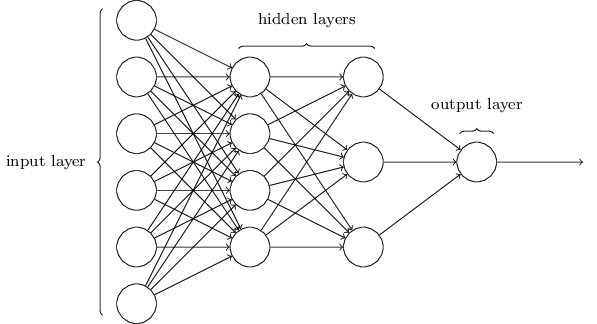
\includegraphics[scale=0.35]{./images/neural_net.png}
 \caption{{\it A common representation of a neural network: a single node works as the perceptron described before. The network is composed by the input layer, the hidden layers and the output layer. The depth of the network is determined by the number of hidden layers.}}
 \label{fig:ann}
\end{figure}

While the number of nodes in the input and output layers is fixed by the data under analysis, the best configuration of hidden layers is still an open problem.

The mathematical generalization from the perceptron is simple, indeed given the $i$-th layer its output vector $\bm{y}_i$ reads:  

\begin{equation}
 \bm{y}_i = \sigma(W_i \bm{y}_{i-1} + \bm{b}_i)
\end{equation}

where $W_i$ is the weights matrix of layer $i$ and $\bm{b}_i$ is the $i$-th bias vector, equivalent to $w_0$ in the perceptron case.
The output of the $i$-th layer becomes the input of the next one until the output layer yields the network's answer. 

As before, $\sigma$ is the activation function which can be different for every node, but it usually differs only from layer to layer. 
How to chose the best activation function is yet to be understood, and most works rely on experimental results.

In a supervised environment, the model output is compared to the desired output ({\it truth}) by means of a cost function. 
An example of cost function is the sum of squared error: 

\begin{equation}
  C(W) = \frac{1}{N} \sum_{j=1}^{N} (y_j - t_j)^2
\end{equation}

where $N$ is the dimensionality of the output space. $C$ is considered as a function of the model's weights only since input data and {\it truth labels} $t$ are fixed.

Those architectures are {\it universal approximators}, that means given an arbitrarly complex function, there is a fully connected neural network that can approximate it.

This type of network is called {\it feed forward} because the information flows directly from the input to the output layer: however, it exists a class of models called {\it Recurrent} where this is not the case anymore and feedback loops are possible, but they are outside the scope of this work. 

\subsection*{Gradient Descent}

To minimize the loss function an update rule for the weights is needed. 
Given a cost funtion $C(w)$, the most simple one is the gradient descent:
\begin{equation}
 w \leftarrow w - \eta \nabla_w C
\end{equation}
The core idea is to modify the parameters by a small step in the direction that minimizes the error function
The lenght of the step is given by the {\it learning rate} $\eta$, which is a hyperparameter chosen by the user, while the direction of the step is given by $-\nabla_w C$, which point towards the steepest descent of the function landscape.

\begin{figure}[H]
 \centering
 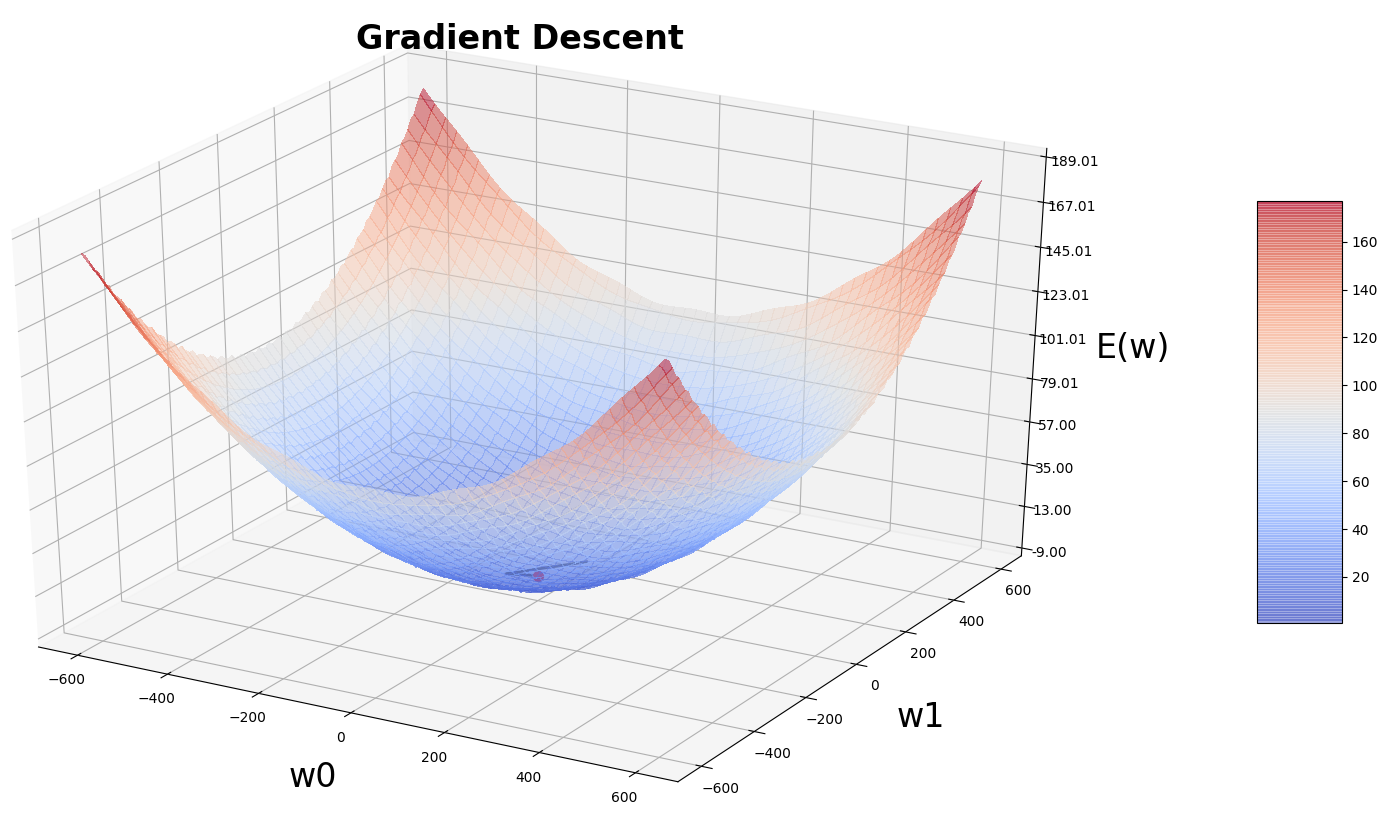
\includegraphics[scale=0.35]{./images/sgd.png}
 \caption{\it Visual example of gradient descent for a model with 2 weights. The idea is to modify the weights to follow the direction of the steepest descent for the landscape of the error function}
 \label{fig:gd}
\end{figure}
The speed at which the algorithm converges to a solution and the precision of said solution are greatly influenced by the update rule. More complex and efficient update rules do exist, but they follow the same idea as the gradient descent.

\subsection*{Error Back Propagation}

The most common algorithm used to compute the updates to weights in the learning phase is the {\it Error Back Propagation}. 
Consider a Neural Network with $L$ total layers, each with a weight matrix $W_l$ with $l = 1, 2, \dots L$.
Given a differentiable cost function $C$, which depends from $W_1, W_2,\dots W_L$, let's define:
\begin{align}
 \bm{z}_l &= W_l \bm{y}_{l-1} + \bm{b}_l  \\ 
 \bm{a}_l &= \sigma(\bm{z}_l)
\end{align}
respectively the {\it de-activated} and {\it activated} output vectors of layer $l$ with $N$ neurons (or $N$ outputs.) and define:
\begin{equation}
 \bm{\delta}_l = (\frac{\partial C}{\partial z_l^1}, \dots , \frac{\partial C}{\partial z_l^N}) 
\end{equation}
the vector of errors of layer $l$. Then we can write the 4 equations of back propagation for the fully-connected neural network \cite{neural-net-nielsen}:
\begin{align}
  &\bm{\delta}_L = \nabla_a C \odot \sigma'(\bm{z}_L) & \mbox{The network error vector} \\ 
  &\bm{\delta}_l = (W_{l+1}^T \bm{\delta}_{l+1}) \odot \sigma'(\bm{z}_l) & \mbox{The error vector for layer $l$} \\
  &\frac{\partial C}{\partial b_l^j} = \delta_l^j & \mbox{The j-th bias update} \\
  &\frac{\partial C}{\partial w_l^{j k}} = a_{l-1}^k \delta_{l}^{j} & \mbox{The update for the weight indexed $j,k$ }
\end{align}
where  $\odot$ is the Hadamard's product.
Those equations can be generalized for others kind of layers, as I will show in the next chapters. 

The full training algorithm is: 
\begin{itemize}
 \setlength\itemsep{-0.3em}
 \item [1] Define the model with random parameters
 \item [2] Compute the output for one of the inputs
 \item [3] Compute the loss function $C(W)$ and the gradients $\frac{\partial C}{\partial w_l^{j k}}$ and $\frac{\partial C}{\partial b_l^j}$ for each $l$.
 \item [4] Updates the parameters following the update rule, 
 \item [5] Iterate from step 2 until the loss is sufficiently small
\end{itemize}

\section{Super Resolution}

The term Super-Resolution (SR) refers to a class of techniques that enhance the spatial resolution of an image, thus converting a given low resolution (LR) image to a corresponding high resolution (HR) one, with better visual quality and refined details.
Image super-resolution is also called by other names like image scaling, interpolation, upsampling and zooming \cite{survey-sr}.
Super resolution can also refers to its ``hardware'' (and best-known) implementation, the {\it super resolution microscopy}, which aim is to overcome the diffraction limit: indeed, the development of super-resolved fluorescense microscopy won a Nobel price in chemistry in 2014, though its technicalities reside outside the scope of this work, which focused on its numerical counterpart.

As described before, the training of a supervised model happens by means of examples: in the case of classification the network is presented with many couples {\it features-label} that compose the {\it train set}. The objective is to find the correct labels for a set of samples never saw before called {\it test set}.

For digital images, the {\it features} are the pixels which compose a 2 dimensional or 3 dimensional (for RGB picture) grid-like structure, the label is usually represented as 1 dimensional vector as large as the binary representation of the number of classes the model is supposed to  discern: a neural network produces a map between a very large {\it features space} and a smaller one.

This behaviour is slightly different for Super-Resolution: indeed, when training a SR model we are talking about {\it image-to-image} processing and as such, both the features space and the labels are images.  
The dataset is built from a single series of high resolution (HR) images which are downsampled to obtain the low resolution (LR) counterpart: the couples LR-HR are fed to the network respectively as input and label just like in a classification problem; this time though, the network will map a smaller feature space into a larger one. 

The models I'm going to use in this work are trained on images downsampled using the {\it bicubic interpolation}.

\subsection{Bicubic Interpolation}

The {\it Bicubic interpolation} is a common algorithm used in image analysis either to downsample or upsample an image. 
This operation is also called \textit{re-scaling} and its purpose is to interpolate the pixel values after a resize of the image, respectively after shrinking or expanding it, e.g as a consequence of zooming. 
The name comes from the highest order of complexity of the operation used in the algorithm, which is a cubic function. 
Given a pixel, the interpolation function evaluates the 4 pixel around it by applying a filter defined as:

\begin{equation}
\hspace*{-1.cm}
k(x) = \frac{1}{6} \left\{ \begin{array}{rc}
  (12 - 9B - 6C) |x|^3 + (-18 + 12B + 6C) |x|^2 + (6 - 2B)           & \mbox{if }        |x| < 1 \\
  (−B − 6C) |x|^3 + (6B + 30C) |x|^2 + (−12B − 48C) |x| + (8B + 24C) & \mbox{if } 1 \leq |x| < 2 \\
  0                                                                  & \mbox{otherwise}         \\
  \end{array}
  \right.
\end{equation}
 
where $x$ identifies each pixel below the filter.
Common values used for the filter parameters are $B=0$ and $C=0.75$ (used by \textsf{OpenCV} library) or $B=0$ and $C=0.5$ used by \textsf{Matlab} and \textsf{Photoshop}.
The scale factor of the down/up sampling can assume different values according to the user needs; for this work, I used an upsampling factor of $\times 2$ and $\times 4$ and the algorithm is from the \textsf{Python} version of the library \textsf{OpenCV} \cite{OpenCV}. 
The main aims of SR algorithms are to provide a better alternative to standard upsampling and obtain a better quality image both from a qualitative (visual perception) and a quantitative poin of view. 

\subsection{Image Quality}

While the human eye is a good qualitative evaluator, it is possible to define different quantitative measures between two images to quantify their similiraties.

\subsection*{PSNR}

One of the most common in Image Analysis is the {\it Peak Signal To Noise Ratio} or PSNR. 
It is usually employed to quantify the recostruction capabilities of an algorithm given a lossy compression, w.r.t the original image. The mathematical espression reads: 

\begin{equation}
 PSNR = 20 \cdot \log_{10} (\frac{max(I)}{MSE})
\end{equation}

where $max(I)$ is the maximum available value for the image $I$, namely $1$ for floating point representation and $255$ for an integer one. 
$MSE$ is the {\it Mean Squared Error}, which is a common metrics in data analysis used to quantify the mean error of a model. It is defined as:

\begin{equation}
 MSE = \frac{1}{HW}\sum_{i=1}^{H} \sum_{j=1}^W (I(i, j) - K(i,j))^2
\end{equation}
 
where $H$ and $W$ are the spatial dimensions of the original image $I$ and the recostruction $K$. 
The metric can be generalized to colored image by simply adding the depth (RGB channel) dimension.

Even though an higher PSNR generally means an higher recostruction quality, this metric may performs poorly compared to other quality metrics when it comes to estimate the quality as perceived by human eyes. An increment of $0.25$ in PSNR corresponds to a visible improvement.
 
\subsection*{SSIM}

Another common metric is the {\it Structural SIMilarity index} or SSIM. It has been developed to evaluate the structural similraties between two images,  while incorporating important perceptual phenomena, including luminance and contrast terms. For that, it should be more representative of the qualitative evaluation as seen by humans.
The SSIM index is defined as: 

\begin{equation}
 SSIM(I, K) = \frac{1}{N} \sum_{i=1}^{N} SSIM_i(x_i, y_i)
\end{equation}

Where $N$ is the number of windows in the images, usually of size $11 \times 11$ or $8 \times 8$. For every box, the index is: 

 \begin{equation}
    \hspace{-0.75cm}
    SSIM(x_i, y_i) = \frac{(2\mu_x\mu_y + c_1)(2\sigma_{xy} + c_2)}{ ({\mu_x}^2 + {\mu_y}^2 + c_1)({\sigma_x}^2 + {\sigma_y}^2 + c_2) },
    \label{SSIM}
\end{equation}

where $x$ and $y$ are two equally-sized regions in two different images, $\mu$ is the average value in the region, $\sigma^2$ is the variance, $\sigma_{xy}$ is the covariance between the regions and $c_1$ and $c_2$ are two constants to stabilize the division.

Both SSIM and PSNR can be useful in Deep Learning applications as target functions or as post-training quality measures. 
To compute PSNR and SSIM I used the function of the Python library {\it scikit image} \cite{scikit}, for their precision, efficency and ease to use.

SR pre-trained models will be evaluated in their reconstruction capabilities against the bicubic interpolation using as benchmark an available dataset of NMR images of brain. 
I'd like to point out that the deep learning architecture tested in this work are trained  on general purpose datasets which are very different from biomedical pictures available:  the first problem is that MRI images are single channeled (gray-scaled) as opposed to the RGB images which those models are trained on, however this can be easily solved by artificially add depth by concatenating the same image 3 times; by doing so, the models elaborate tree different outputs that can be compared against each others.  
The second issue is that the models never had a chance to learn the particular shapes contained in animals' brain: although that could be seen as a major drawback, their generalization capability should be sufficient to perform well even outside their optimal "environment". 
The datasets will be discussed in later chapters.

\section{Nuclear Magnetic Resonance}

The term NMR identifies an experimental technique called Nuclear Magnetic Resonance.
It has been indipendently developed by two reserch groups led Felix Bloch and Edward Purcell, both awarded with the Nobel prize in Physics in 1952. 
Initially, NMR was tied to studies in fundamental physics and particularly to solid state physics: its theoretical and technological evolution in the years allowed numerous applications also in the biological and medical fields.    
Differently from other invasive techniques from nuclear medicine or radiology, which employ ionising radiations dangerous for the organism, in NMR the only source of energy administration is represented by two types of electromagnetic fields: static and radio-frequency.
By applying those fields to nuclei which posses magnetic properties it is possible to analyze the macroscopic structure of the sample. 
The most used nuclei are ${}^1H, {}^2H, {}^{31}P, {}^{23}Na, {}^{14}N, {}^{13}C, {}^{19}F$, which is really advantegeous in the biological field, given that the subjects are most likely rich in $H_2O$, therefore in ${}^1H$. 
This allows to detect signals of large intensity from the samples and measure a high ratio signal/noise even with few acquisitions.

As stated before, NMR is applied to nuclei which posses magnetic properties, therefore they have an angular momentum $\bm{I}$ (spin) associated with a magnetic momentum $\bm{\mu} = \gamma(\frac{h}{2\pi})\bm{I}$ where $\gamma$ is the gyromagnetic ratio, which depends from the nucleus.

Considering an ensemble of ${}^1H$ with $I = \frac{1}{2}$, if a static magnetic field $\bm{B}_0 = H_0 \hat z$ is applied, the magnetic momenta of the nucleus will orientate themselves along the parallel or anti-parallel direction of the fields, assuming two discrete values of energy. 
According to Boltzmann statistic, the majority of nuclei will orientate in such a way to minimize the energy (parallel to $\bm{B}_0$).

The energy difference between the two level is given by: 

\begin{equation}
 \Delta E = \gamma \left(\frac{h}{2\pi}B_0\right) = \left(\frac{h}{2\pi}\omega_0\right)
 \label{eq:res-cond}
\end{equation}

where $\omega_0$ is the Larmor Frequency.
The energy that must be given to perturb the system from its equilibrium condition follow the resonance condition \ref{eq:res-cond}. 
The perturbation is represented by a radio-frequency electromagnetic field $\bm{B}_1$ perpendicular to $\bm{B}_0$, oscillating at the Larmor frequency of the system $\omega_0$.
After removal of the perturbation, it is possible to measure the relaxation times $T_1$ and $T_2$ of the longitudinal and trasversal components of the nuclei magnetization. 

For the nuclei, the temporal evolution of $\bm{\mu}$ under the influence of the static fields $\bm{B}_0$ is given by:

\begin{equation}
  \frac{d \bm{\mu}}{d t} = \gamma \bm{\mu} \times \bm{B}_0
\end{equation}

and by separating the three components it yields:

\begin{align}
  \frac{d \mu_x}{d t} &= \gamma \mu_x B_0 \\ 
  \frac{d \mu_y}{d t} &= \gamma \mu_y B_0 \\
  \frac{d \mu_z}{d t} &= 0
\end{align}

which highlights how the magnetic moment performs a precession around the $z$ axis with frequency $\omega_0 = \gamma B_0$

The radio-frequency magnetic field $\bm{B}_1$, with $B_1 << B_0$ and frequency $\omega$ is perpendicular to $\bm{B}_0$ lying in the $xy$ plane and can be obtained by an oscillating fields generated by a coil traversed by a radio-frequency current.

In the most general case of nuclear magnetization, if the system is influenced by field $\bm{B}_0$ and $\bm{B}_1$ it is in a non-equilibrium condition described by the {\it Block Equations} for each components:

\begin{align}
 \frac{d M_{z}}{d t}  &= - \frac{M_z(t) - M_z(0)}{T_1} & \mbox{longitudinal relaxation}\\
 \frac{d M_{xy}}{d t} &= - \frac{M_{xy}(t) - M_{xy}(0)}{T_2} & \mbox{trasversal relaxation}
\end{align}

Their integration brings: 

\begin{align}
 M_z(t)    &= M_z(0)exp\left(\frac{-t}{T_1}\right) + M_z(0)\left(1 - exp\left(\frac{-t}{T_1}\right)\right) \\
 M_{xy}(t) &= M_{xy}(0)exp\left(\frac{-t}{T_2}\right)
\end{align}

Bloch's equations are fundamental for the choice of the sequence of excitation and subsequent acquisition and elaboration of the signal.
Once the perturbation action ends, its possible to follow the de-excitation of the macroscopic magnetization M , which tends to realign to the field $\bm{B}_0$. The signal produced by the variation of M is measured by an induction electromagnetic coil around the sample in an ortogonal direction w.r.t the static field.
The NMR signal, called FID (Free Induction Decay), is approximately monochromatic and oscillates at Larmor frequency, decaying exponenetially as a functio of $T_2$. 
For Image formation (MRI), excitation sequences are opportunely chosen in such a way to emphasize the dipendence of FID from three parameters: protonic density $\rho$, $T_1$ and $T_2$.
\\
MRI can be differentiated in two types: T1-weighted sequences and T2-weighted sequences, which show different information.
The former are considered the most ``anatomical'' and result in images that most closely appoximate the appearences of tissues: fluid  have low signal intensity (black), muscle and gray-matter has a intermediate signal intensity (grey) and fat and white-matter have a high signal intensity (white).
\\
The latter instead, have a high signal intensity for fluid an fat, an intermediate intensity for muscle and grey-matter, and low intensity for white-matter, which appears dark-ish.
\\
In figure \ref{fig:diff-t1-t2} is shown a comparison between the two:

\begin{figure}[H]
 \centering
 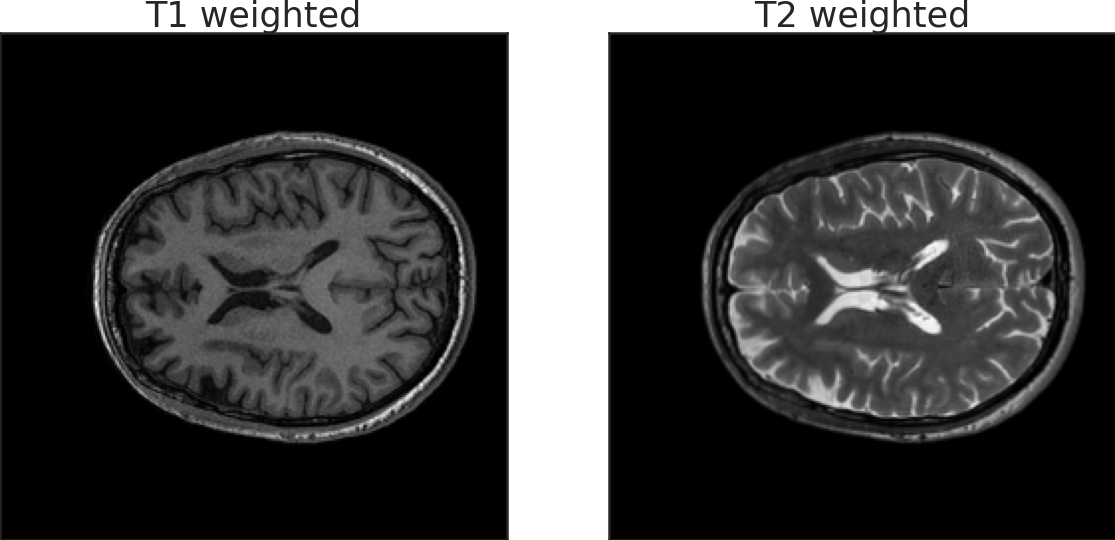
\includegraphics[scale=0.4]{./images/t1_t2_diff.png}
 \caption{\it Comparison between a T1-weighted slice (left) and a T2-weighted slice (right) for the same patient}
 \label{fig:diff-t1-t2}
\end{figure}


\chapter{Algorithms}

A wide range of documentations and implementations have been written on the topic of Deep Learning and it is more and more difficult to move around the different sources.
In recent years, leaders in DL applications became the multiple open-source \textsf{Python} libraries available on-line as \textsf{Tensorflow}~\cite{tensorflow2015-whitepaper}, \textsf{Pytorch}~\cite{paszke2017automatic} and \textsf{Caffe}~\cite{Jia:2014:Caffe}.
Their portability and efficiency are closely related on the simplicity of the \textsf{Python} language and on the simplicity in writing complex models in a minimum number of code lines.
Only a small part of the research community uses deeper implementation in \textsf{C++} or other low-level programming languages and between them should be mentioned the \textsf{darknet project} of Redmon J. et al. which has created a sort of standard in object detection applications using a pure \textsf{Ansi-C} library.
The library was developed only for Unix OS but in its many branches (literally \emph{forks}) a complete porting for each operative system was provided.
The code is particularly optimized for GPUs using CUDA support, i.e only for NVidia GPUs.
It is particularly famous for object detection applications since its development is tightly associated to an innovative approach at multi-scale object detections called YOLO (\emph{You Only Look Once}), that recently reached its fourth release \cite{yolov4}.
The libraries built during the develompment of this thesis are all inspired by the efficiency and modularity of darknet and make an effort to not only replicate but expand on their work, both in performances, functionalities and solved issues.

In this section I will describe the mathematical background of these models and 
to most theoretical explanation  discuss the numerical problems associated, tied to the development of two new libraries: \textsf{NumPyNet} \cite{NumPyNet} and \textsf{Byron} \cite{Byron}.

\section{Frameworks}

\textsf{NumPyNet} is born as an educational framework for the study of Neural Network models.
It is written trying to balance code readability and computational performances and it is enriched with a large documentation to better understand the functionality of each script.
The library is written in pure \textsf{Python} and the only external library used is \textsf{Numpy}~\cite{Numpy} (a base package for the scientific research).
As I will show in the next sections, \textsf{Numpy} allows a relatively efficient implementation of complex algorithms by keeping the code as similar as possible to the mathematic computations involved.

Despite being supplied by wide documentations, it is often difficult for novel users to move around the many hyper-links and papers cited in all common libraries.
\textsf{NumPyNet} tries to overcome this problem with a minimal mathematical documentation associated to each script and a wide range of comments inside the code.

An other "problem" to take into account is associated to performances.
On one hand, libraries like \textsf{Tensorflow} are certainly efficient from a computational point-of-view and the numerous wraps (like \emph{Keras}) guarantee an extremely simple user interface.
On the other hand, the deeper functionalities of the code and the implementation strategies used are unavoidably hidden behind tons of code lines.
In this way the user can perform complex computational tasks using the library as black-box package.
\textsf{NumPyNet} wants avoid this problem using simple \textsf{Python} codes, with extreme readability also for new users, to better understand the symmetry between mathematical formulas and code.
The simplicity of this library allows us to give a first numerical analysis of the model functions and, moreover, to show the results of each function on an image to better understand the effects of their applications on real data.
Each \textsf{NumPyNet} function was tested against the equivalent \textsf{Tensorflow} implementation, using an automatic testing routine through \textsf{PyTest}~\cite{PyTest}.
The full code is open-source on the \textsf{Github} page of the project.
Its installation is guaranteed by a continuous integration framework of the code through \textsf{Travis CI} for Unix environments and \textsf{Appveyor CI} for Windows OS.
The library supports \textsf{Python} versions $\ge2.7$.

As term of comparison we discuss the more sophisticated implementation given by the \textsf{Byron} library.
\textsf{Byron} (\emph{Build YouR Own Neural network}) library is written in pure \textsf{C++} with the support of the modern standard \textsf{C++17}.
We deeply use the \textsf{C++17} functionality to reach the better performances and flexibility of our code.
What makes \textsf{Byron} an efficient alternative to the competition is the complete multi-threading environment in which it works.
Despite the most common Neural Network libraries are optimized for GPU environments, there are only few implementations which exploit the full set of functionalities of a multiple CPUs architecture.
This gap discourages multiple research groups on the usage of such computational intensive models in their applications.
\textsf{Byron} works in a fully parallel section in which each single computational function is performed using the entire set of available cores.
To further reduce the time of thread spawning, and so optimize as much as possible the code performances, the library works using a single parallel section which is opened at the beginning of the computation and closed at the end.

The \textsf{Byron} library is released under \textsf{MIT} license and publicly available on the \textsf{Github} page of the project.
The project includes a list of common examples like object detection, super resolution, segmentation.
The library is also completely wrapped using \textsf{Cython} to enlarge the range of users also to the \textsf{Python} ones.
The complete guide about its installation is provided; the installation can be done using \textsf{CMake}, \textsf{Make} or \textsf{Docker} and the \textsf{Python} version is available with a simple \textsf{setup.py}.
The testing of each function is performed using \textsf{Pytest} framework against the \textsf{NumPyNet} implementation (faster and lighter to import than \textsf{Tensorflow}) \cite{nicotesi}.

\section{Layers}

As described above, a neural network can be considered as a composition of function: for this reason every Deep Learning framework (e.g. Keras/Tensorflow, Pytorch, Darknet) implement each function as an independent object called {\it Layer}. In Byron and NumPyNet, each layer contains at least 3 methods:
\begin{itemize}
 \setlength\itemsep{-0.3em}
 \item {\bf forward} the forward method compute the output of the layer, given as input the previous output. 
 \item {\bf backward} the backward method is essential for the training phase of the model: indeed, it computes all the updates for the layer weights and backpropagates the error to the previous layers in the chain.
 \item {\bf update} the update method applies the given update rules to the layer's weights.
\end{itemize}
By stacking different kind of layers one after another, it is possible to build 
complex models with tens of millions of parameters. 
For the purposes of this work, I'm going to describe layers used in super resolution, however, Byron is developed also for different applications (object detection, classification, segmentation, style transfer, natural language processing etc...) and as such, many more layers are available.   

\subsection*{Convolutional Layer}

A Convolutional Neural Network (CNN) is a specialized kind of neural network for processing data that has known grid-like topology \cite{Goodfellow-et-al-2016}, like images, that can be considered as a grid of pixels.
The name indicates that at least one of the functions employed by the network is a convolution. In a continuos domain the convolution between two functions $f$ and $g$ is defined as: 
\begin{equation}
 (f * g)(t) = \int_{-\infty}^{+\infty} f(\tau)g(t-\tau)d\tau
\end{equation}
The first function $f$ is usually referred to as the input and the second function $g$ as kernel. 
For Image Processing applications we can define a 2-dimensional discrete version of the convolution in a finite domain using an image $I$ as input and a 2 dimensional kernel $k$:
\begin{equation}
 C[i, j] = \sum_{u=-N}^N \sum_{v=-M}^M k[u, v] \cdot I[i-u, j-v]
 \label{eq:conv}
\end{equation}
where $C[i, j]$ is the pixel value of the output image and $N$, $M$ are the kernel dimensions.
Practically speaking, a convolution is performed by sliding a kernel of dimension $N \times M$ over the image, each kernel position corresponds to a single output pixel, the value of which is calculated by multiplying together the kernel value and the underlaying pixel value for each cell of the kernel and summing all the results, as shown in figure \ref{fig:convolution}:

\begin{figure}[H]
 \centering
 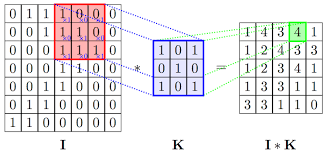
\includegraphics[scale=0.5]{./images/conv.png}
 \caption{\it Visual representation of a convolution of an Image $I$ with a kernel of size 3}
 \label{fig:convolution}
\end{figure}

The convolution operation is also called $filtering$. By chosing the right kernel (filter) it is possible to highlight different features. For this reason the convolution operation is commonly used in image analysis: some of the most common applications are denoising, edge detection and edge enhancement. 

The convolutional layer (CL) object is the most used layer in DL image analysis, therefore its implementation must be as efficient as possible.
Its purpose is to perform multiple (sometimes thousands) convolution over the input to extract different high-level features, which are compositions of many low-level attributes of the image (e.g edges, simple shapes).
In the brain/neuron analogy, every entry in the output volume can also be interpreted as an output of a neuron that looks at only a small region, the neuron's {\it receptive field} in the input and shares parameters with all the neuron spatially close.
As more CLs are stacked, the receptive field of a single neuron grows and with that, the complexity of the features it is able to extract.
The local nature of the receptive field allows the models to recognize features regardless of the position in the images. In other words, it is independent from translations \cite{Goodfellow-et-al-2016}. 

The difference from a traditional convolutional approach is that instead of using pre-determined filters, the network is supposed to learn its own.
A CL si defined by the following parameters: 

\begin{itemize}
 \setlength\itemsep{-0.2em}
 \item [-] {\bf kernel size}: it is the size of the sliding filters. The depth of the filters is decided by the depth of the input images (which is the number of channels.). The remanining 2 dimensions (width and height) can be indipendent from one another, but most implementations require squared kernels.
 \item [-] {\bf strides}: defines the movement of the filters. With a low stride (e.g. unitary) the windows tends to overlap. With high stride values we have less overlap (or none) and the dimension of the output decrease.
 \item [-] {\bf number of filters}: is the number of different filters to apply to the input. It also indicates the depth of the output.
 \item [-] {\bf padding}: is the dimension of an artificial enlargement of the input to allow the application of filters on borders. Usually, it can be interpreted as the number of rows/columns of pixel to add to the input, however some libraries (e.g Keras) consider it only as binary: in case is true, only the minimum number of rows/columns are appended to keep the same spatial dimension.
\end{itemize}
Given the parameters, it is straightforward to compute the number of weights and bias needed for the initialization of the CL: indeed, suppose an image of dimensions $(H, W, C)$ slided by $n$ different 3-D filters of size $(k_x, k_y)$ with strides $(s_x, s_y)$ and padding $p$, then:
\begin{align}
 \# weights &= n \times k_x \times k_y \times C \\
 \# bias &= n
\end{align}
Note that the number of weights does not depend on the input spatial size but only on its depth. It is important because a fully convolutional network can receives images of any size as long as they have the correct depth. Moreover, using larger inputs do not requires more weights, as is the case for fully connected structure. 

The output dimensions are $(out\_H, out\_W, n)$ where:
\begin{align}
 out\_H &= \lfloor\frac{H - k_x + p}{s_x}\rfloor + 1 \\
 out\_W &= \lfloor\frac{W - k_y + p}{s_y}\rfloor + 1
\end{align}

Even if the operation can be implemented as described above in equation \ref{eq:conv}, this is never the case: it is certainly easier but also order of magnitude slower than more common algorithms.
A huge speed up in performances is given by realising that a discrete convolution can be viewed as a single matrix multiplication. The first matrix has as rows each filters of the CL, while the second matrix has as columns every windows of the image traversed by the kernels, as shown in figure \ref{fig:im2col}.

\begin{figure}[h]
 \centering
 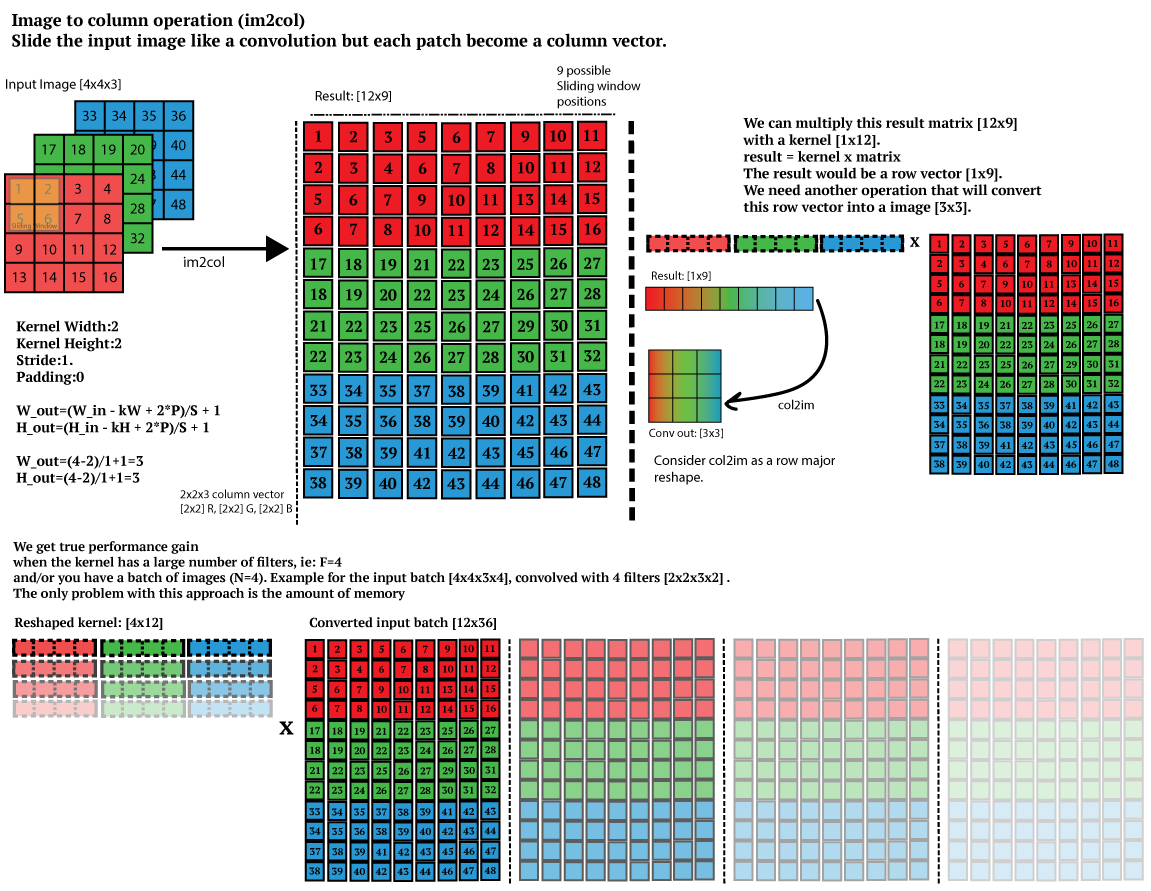
\includegraphics[scale=0.35]{./images/im2col.png}
 \caption{\it Scheme of the im2col algorithm using a $2 \times 2 \times 3$ filter with stride 1 on a $4 \times 4 \times 3$ image. The matrix multiplication is between a $n \times 12$ and a $12 \times 9$ matrixes.}
 \label{fig:im2col}
\end{figure}

This re-arrengement is commonly called im2col. The main downside is that a lot more memory is needed to store the newly arranged matrix.
The larger the number of kernels, the higher is the time gain of this implementation over a naive one.  

Another important optimization comes from linear algebra considerations and is called {\it Coppersmith-Winograd algorithm}, which was designed to optimize the matrix product.
Suppose we have an input image of just 4 elements and a 1-D filter mask with size 3:

\begin{equation}
\mbox{img} = \left[\begin{array}{cccc} d0 & d1 & d2 & d3 \end{array}\right] \quad\quad \mbox{weights} = \left[\begin{array}{ccc} g0 & g1 & g2 \end{array}\right]
\end{equation}
\\
we can now use the \textsf{im2col} algorithm previously described and reshape our input image and weights into

\begin{equation}
\mbox{img} = \left[
\begin{array}{ccc}
d0 & d1 & d2 \\
d1 & d2 & d3
\end{array}
\right],
\quad\quad
\mbox{weights} = \left[
\begin{array}{c}
g0 \\
g1 \\
g2
\end{array}
\right]
\end{equation}
\\
given this data, we can simply compute the output as the matrix product of this two matrices:

\begin{equation}
\mbox{output} = \left[
\begin{array}{ccc}
d0 & d1 & d2 \\
d1 & d2 & d3
\end{array}
\right]
\left[
\begin{array}{c}
g0 \\
g1 \\
g2
\end{array}
\right] = \left[
\begin{array}{c}
d0 \cdot g0 + d1 \cdot g1 + d2 \cdot g2 \\
d1 \cdot g0 + d2 \cdot g1 + d3 \cdot g2 
\end{array}
\right]
\end{equation}
\\
The Winograd algorithm rewrites this computation as follow:

\begin{equation}
\mbox{output} = \left[
\begin{array}{ccc}
d0 & d1 & d2 \\
d1 & d2 & d3
\end{array}
\right]
\left[
\begin{array}{c}
g0 \\
g1 \\
g2
\end{array}
\right] = \left[
\begin{array}{c}
m1 + m2 + m3 \\
m2 - m3 - m4
\end{array}
\right]
\end{equation}
\\
where

\begin{equation}
\begin{aligned}
m1 = (d0 - d2)g0\quad\quad m2 = (d1 + d2)\frac{g0 + g1 + g2}{2}
\\
m4 = (d1 - d3)g2\quad\quad m3 = (d2 - d1)\frac{g0 - g1 + g2}{2}
\end{aligned}
\end{equation}

The two fractions in $m2$ and $m3$ involve only weight's values, so they can be computed once per filter. Moreover, the normal matrix multiplication is composed of 6 multiplications and 4 addition, while the winograd algorithm reduce the number of multiplication to 4, that is very significant, considering that a  single multiplication takes 7 clock-cycles and an addition only 3. 
In Byron we provide the winograd algorithm for square kernels of size 3 and stride 1, since it is one of the most common combinations in Deep Learning and the generalization is not straightforward.

In the backward operation is important to remember that each weight in the filter contributes to each pixel in the output map. 
Thus, any change in a weight in the filter will affect all the output pixels. 
Note that the backward function can still be seen as a convolution between the input and the matrix of errors $\delta^l$ for the updates and as a full convolution between $\delta^l$ and the flipped kernel for the error $\delta^{l-1}$.
In the case the windows of kernels overlap, updates are the sum of all the contributing elements of $\delta^l$.

\subsection*{Pooling}

Pooling operations are down-sampling operations, so that the spatial dimensions of the input are reduced. Similarly to what happens in a CL, in pooling layers a 3-D kernel of size $k_x \times k_y \times C$ slides across an image of size $H \times W \times C$, however the operation performed by this kind of layers is fixed and does not change during the course of training.
The two main pooling functions are max-pooling and average-pooling: as suggested by the names, the former  
returns the maximum value of every window of the images super-posed by the kernel, as shown in figure \ref{fig:maxpool}.

\begin{figure}[h]
 \centering
 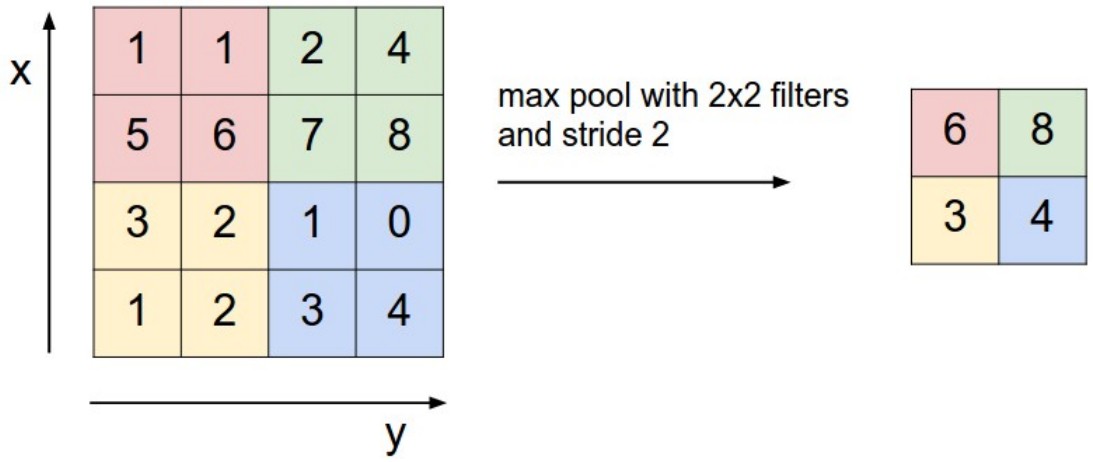
\includegraphics[scale=0.35]{./images/maxpool.png}
 \caption{\it Scheme of maxpool operations with a kernel of size $2 \times 2$ and stride $2$ over an image of size $4 \times 4$. Picture from CS231n}
 \label{fig:maxpool}
\end{figure}

The latter instead, returns the average value of the window and can be seen as a convolution where every weight in the kernel is $\frac{1}{k_x \cdot k_y}$.
The results expected from an Average pooling operations are shown in figure \ref{fig:avgpool:ex}.

\begin{figure}[h]
 \centering
 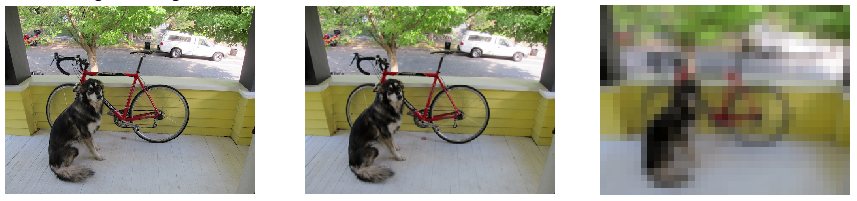
\includegraphics[scale=0.7]{./images/avgpool_layer.png}
 \caption{\it Average pooling applied to a test image: (left) the original image, (center) average pooling with a $3 \times 3$ kernel, (right) average pooling with a $30 \times 30$ kernel. The images have been obtained using NumPyNet}
 \label{fig:avgpool:ex}
\end{figure}

Other popular pooling functions include the $L^2$ norm of a rectangular neighborhood or a weighted average based on the distance from the central pixel.

A typical block of a convolutional network consists of three stages: In the first stage a CL performs several convolutions in parallel, in the second stage each convolution result is run through a non-linear activation function (sometimes called {\it detector}) and in the third stage a pooling function is used to further modify the output. 
The modification brought by pooling is helpful in different ways: first of all, it is a straightforward computational performance improvement, since less features also means less operations. 
Moreover, in all cases, pooling helps to make representation approximately invariant to small translation of the input and invariance to local translation can be a useful property if the objective is to decide wether a feature is present rather than where it is located \cite{Goodfellow-et-al-2016}.
The reductions of features can also prevent over-fitting problems during training, improving the general performances of the model. 

A pooling layer is defined by the same parameters as a CL, minus the number of filters; moreover, also the output dimensions for Pooling layers are the same as for CLs, however, they have no weights to be trained.

Due to the similarities with the CL it is possible to implement a pooling layers through the im2col algorithm, as an example, the NumPyNet implementation shown in the snippet below make use of the function \texttt{asStride} to create a \texttt{view} of the input array: 

\lstset{style=snippet}
\begin{lstlisting}[language=Python, caption=NumPyNet version of Maxpool function, label=code:py_avgpool]
import numpy as np

class Maxpool_layer(object):

  def __init__(self, size=(3, 3), stride=(2, 2)):

    self.size = size
    self.stride = stride
    self.batch, self.w, self.h, self.c = (0, 0, 0, 0)
    self.output, self.delta = (None, None)

  def _asStride(self, input, size, stride):

    batch_stride, s0, s1 = input.strides[:3]
    batch,        w,  h  = input.shape[:3]
    kx, ky     = size
    st1, st2   = stride

    view_shape = (batch, 1 + (w - kx)//st1, 1 + (h - ky)//st2) + input.shape[3:] + (kx, ky)

    strides = (batch_stride, st1 * s0, st2 * s1) + input.strides[3:] + (s0, s1)

    subs = np.lib.stride_tricks.as_strided(input, view_shape, strides=strides)
    
    return subs

  def forward(self, input):

    kx , ky  = self.size
    st1, st2 = self.stride
    _, w, h, _ = self.input_shape

    view = self._asStride(input)

    self.output = np.nanmax(view, axis=(4,5))

    new_shape = view.shape[:4] + (kx*ky, )

    self.indexes = np.nanargmax(view.reshape(new_shape), axis=4)

    self.indexes = np.unravel_index(self.indexes.ravel(), shape=(kx, ky))

    self.delta = np.zeros(shape=self.out_shape, dtype=float)

    return self

\end{lstlisting}

A \texttt{view} is a special \texttt{numpy} object which retains the same information of the original array arranged in a different way, but without occupying more memory. In this case, the re-arrengement is very similar to an im2col, with the only difference that we are not bound to any number of dimensions. The resulting tensor has indeed 6 dimensions.
Since no copy is produces in this operation we can obtain a faster execution.

In pooling layer the backward function is similar to what we saw for convolutional layers, this time we don't have to compute the weights updates though, only the error to back-progate along the network.
For maxpool layers, only the maximum input pixel for every window is involved in the backward pass. Indeed, if we consider the simple case in which the forward function is: 

\begin{equation}
 m = max(a, b)
\end{equation}

and, as described in the dedicated chapter, we know that $\frac{\partial C}{\partial m}$ is the error passed back from the next layer: the objective is to compute $\frac{\partial C}{\partial a}$ and $\frac{\partial C}{\partial b}$. 
If $a > b$ we have: 

\begin{equation}
 m = a \quad \Rightarrow \quad \frac{\partial C}{\partial m} = \frac{\partial C}{\partial a}
\end{equation}
$m$ does not depends on $b$ so $\frac{\partial C}{\partial b} = 0$.

So the error is passed only to those pixels which value is maximum in the considered window, the other are zeros. 
In figure \ref{fig:maxpool:ex} an example of forward and backward pass for a maxpool kernel of size 30 and stride 20.

\begin{figure}[H]
 \centering
 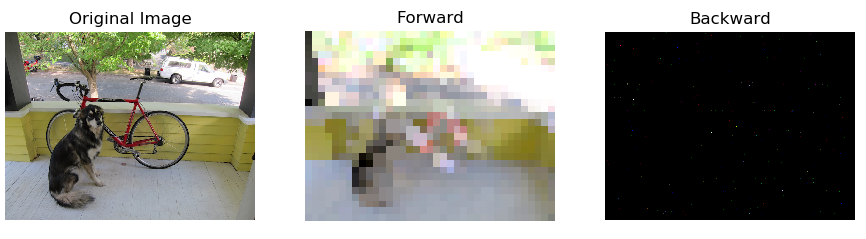
\includegraphics[scale=0.53]{./images/maxpool_30_20.png}
 \caption{\it Max pooling applied to a test image: (left) the original image, (center) max pooling with a $30 \times 3$0 kernel and stride $20$, (right) max pooling errors image. Only few of the pixels are responsible for the error backpropagation. 
 The images have been obtained using NumPyNet}
 \label{fig:maxpool:ex}
\end{figure}

The backward pass for the average pool layer is the same as for the CL, considering that in this case the ``weights'' are fixed.

% According to \cite{nopool}, it is possible to build models exclusively out of convolutional layers without the need for pooling and reach state-of-the art performances 

\subsection*{Shortcut Connections}

An important advancement in network architecture has been brought by the introduction of Shortcut (or Residual) Connections \cite{residual}. It is well know that deep models suffer from {\it degradation problems} after reaching a maximum depth. Adding more layers, thus increasing the depth of the model, saturates the accuracy which eventually starts to rapidly decrease. 
The main cause of this dergradation is not overfitting, but numerical instability tied to gradient backpropagation: indeed, as the gradient is back-propagated through the network, repeated multiplications can make those gradients very small or, alternatevely, very big,
This problem is well known in Deep Learning and takes the name of {\it vanishing}/{\it exploding gradients} and it makes almost impossible to train very large models, since early layers may not learn anything even after hundreds of epochs.
A residual connection is a special shortcut which connects 2 different part of the network with a simple linear combination.
Instead of learning a function $F(x)$ we try to learn $H(x) = F(x) + x$, as shown in figure \ref{fig:shortcut}:

\begin{figure}[h]
 \centering
 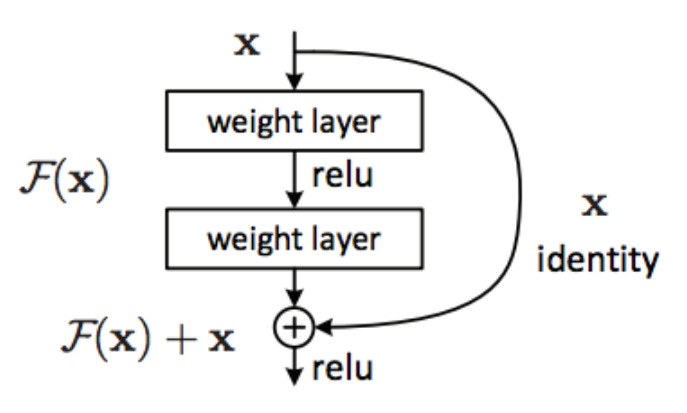
\includegraphics[scale=0.4]{./images/shortcut.png}
 \caption{\it Scheme of the shortcut layer as designed by the authors \cite{residual}. The output of the second layer become a linear combination of the input x and its own output.}
 \label{fig:shortcut}
\end{figure}
During the back propagation the gradient of higher layers can easily pass to the lower layers, without being mediated, which may cause vanishing or exploding gradient.
\\
Both in NumPyNet and Byron, we chose to generalize the formula as: 

\begin{equation}
 H(x_1, x_2) = \alpha x_1 + \beta x_2
\end{equation}
Where $x_1$ is the output of the previous layer and $x_2$ is the output of the layer selected by \texttt{index} paramter. Indeed, even the shortcut connection can be implemented as a stand-alone layer, defined by the following parameters:

\begin{itemize}
 \setlength\itemsep{-0.2em}
 \item {\bf index} is the index of the second input of this layer $x_2$ (the first one $x_1$ is the output of the previous layer).
 \item {\bf alpha} the first coefficient of the linear combination, multiplied by $x_1$.
 \item {\bf beta} the second coefficient of the linear combination, multiplied by $x_2$.
\end{itemize}
.
The backward function is simply:

\begin{equation}
 \frac{\partial C}{\partial x_1} = \frac{\partial C}{\partial H}\frac{\partial H}{\partial x_1} = \delta \cdot \alpha
\end{equation}
for the first layer and:

\begin{equation}
 \frac{\partial C}{\partial x_2} = \frac{\partial C}{\partial H}\frac{\partial H}{\partial x_2} = \delta \cdot \beta
\end{equation}
for the second layer. Again, $\delta$ is the error backpropagated from the next layer. 
Residuals connections were first introduced for image classification problems, but they rapidly become part of numerous models for every kind of application tied to Image Analysis.

\subsection*{Pixel Shuffle}

Using pooling and convolutional layers with non unitarian strides is a simple way to downsample the input dimension. 
For some applications though, we may be interested in upsampling the input, for example: 

\begin{itemize}
 \setlength\itemsep{-0.2em}
 \item in image to image processing (input and output are images of the same size) it is common to perform a compression to an internal encoding (e.g Deblurring, U-Net Segmentation). 
 \item project feature maps to a higher dimensional space, i.d. to obtain a image of higher resolution (e.g Super-Resolution)
\end{itemize}
for those purposes the {\it transposed convolution} (also called {\it deconvolution}) was introduced. 
The transposed convolution can be treated as a normal convolution with a sub-unitarian stride, by upsampling the input with empty rows and columns and then apply a single strided convolution, as shown in figure \ref{fig:deconv}.

\begin{figure}[h]
 \centering
 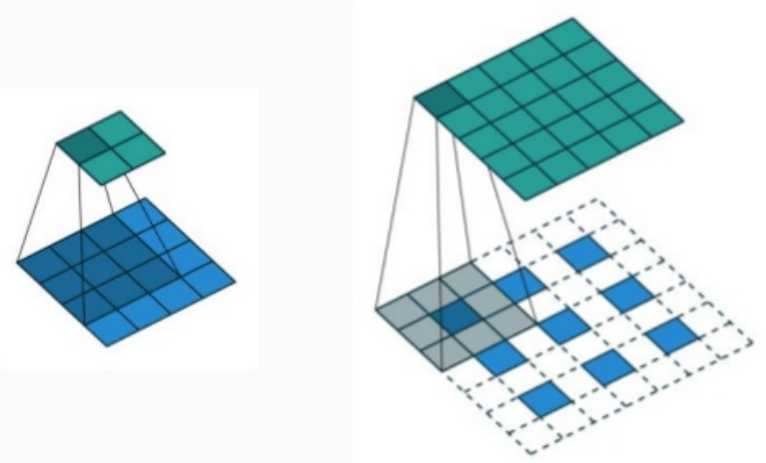
\includegraphics[scale=0.35]{./images/deconv.png}
 \caption{\it example of deconvolution: (left) a normal convolution with size 3 and stride 1, (right) after applying a "zeros upsampling" the convolution of size 3 and stride 1 become a deconvolution}
 \label{fig:deconv}
\end{figure}

Although it works, the transposed convolution is not efficient in terms of computational and memory cost, therefore not suited for modern convolutional neural networks. 
An alternative is the recently introduced {\it sub-pixel convolution} \cite{pixelshuffle} (also called Pixel Shuffle). The main advantages over the deconvolution operation is the absence of weights to train: indeed the operation performed by the Pixel Shuffle (PS) Layer is deterministic and it is very efficient if compared to the deconvolution, since it is only a re-arrengement of the pixels. 

Given a scale factor $r$, the PS organizes an input $H \times W \times C \cdot r^2$ into an output tensor $r \cdot H \times r \cdot W \times C$, which generally is the dimension of the high resolution space. 
So, strictly speaking, the PS does not perform any upsample, since the number of pixels stays the same. 
In figure \ref{fig:pixelshuffle1} is shown an example with $C=1$:

\begin{figure}[h]
 \centering
 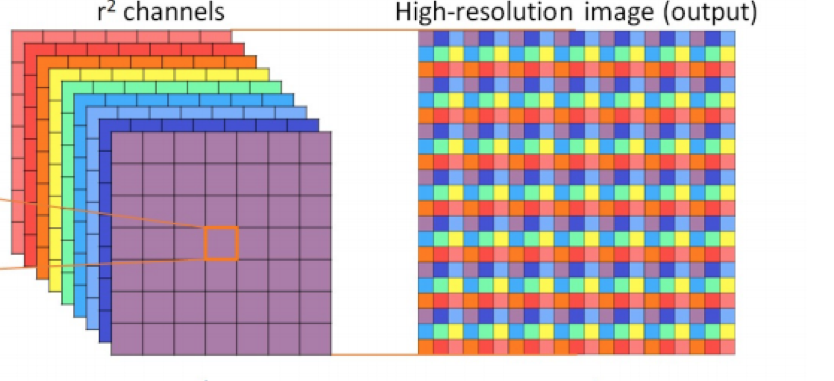
\includegraphics[scale=0.35]{./images/pixelshuffle.png}
 \caption{\it Example of pixel shuffling proposed by the authors \cite{pixelshuffle}. In this example, $r^2$ features maps are re-arranged into a single-channeled high resolution output.}
 \label{fig:pixelshuffle1}
\end{figure}

As suggested by the authors, the best practice to improve performances is to upscale from low resolution to high resolution only at the very end of the model. 
In this way the CL can efficienlty produce an high number of low resolution feature maps that the PS can organize into the final output. 

In both NumPyNet and Byron, the pixel shuffle layer is defined only by the \texttt{scale} parameter, which lead the entire transformation.
In the first case, it is possible to implement forward and backward using the functions \texttt{split}, \texttt{reshape}, \texttt{concatenate} and \texttt{transpose} of the \texttt{numpy} library \cite{Numpy}. 
This implementation has been tested against \texttt{tensorflow}'s \texttt{depth\_to\_space} and \texttt{space\_to\_depth}.
Despite being available in most deep learning library, a low level  \texttt{C++} implementation for the PS algorithm is hard to find. 
In Byron we propose a dynamic algorithm able to work for both \texttt{channel last} and \texttt{channel first} input. 
The algorithm is essentially a re-indexing of the input array in six nested for-loops. The first solution taken into account during the development was the contraction of the loops into a single one using divisions to obtain the correct indexes: however the amount of required divisions weights on the computational performances, given that divisions are the most expensive operation in terms of CPU clock-cycles. 

The backward function of this layer does not involve any gradient computation: instead, it is the inverse of the re-arrengement performed in the forward function.

\subsection*{Batch Normalization}

When training a neural network, the standard approach is to separate the dataset in groups, called {\it batches} or {\it mini-batches}. 
In this way the network can be trained with multiple input at a time and the updates for the weights are usually computed by averaging in the batch.
The number of examples in each batch is called \textit{batch size}: this can varies from 1 to the size of the dataset. 
Using batch sizes different from one is beneficial in several ways. 
First, the gradient of the loss over a mini-batch is a better estimate of the gradient over the train set, whose quality improves as the batch size increases, but using the entire train set can be very costly in terms of memory usage and often impossible to achieve.
Second, it can be much more efficient in modern architecture due to the  parallelism instead of performing M sequential computations for single examples. \cite{batchnorm}

Batch normalization is the operation that normalizes the features of the input along the batch axis, which allows to overcome a phenomenon in Deep Network training called {\it internal covariate shift}: whenever the parameters of the model change, the input distributions of every layer change accordingly.
This behaviour produces a slow down in the training convergence because each layer has to adapt itself to a new distribution of data for each epoch. Moreover, the parameters must be carefully initialized. 
By making the normalization a part of the model architecture, the layer acts also as a regularizer, which in turn allows better generalization perfomances.  

Let's $M$ be the number of examples in the group and $\epsilon$ a small variable added for numerical stability, the batch normalization function is defined as: 

\begin{align}
  &\mu = \frac{1}{M} \sum_{i=1}^{M} x_i \\
  &\sigma^2 = \frac{1}{M} \sum_{i=1}^{M} (x_i - \mu)^2 \\
  &\hat x_i = \frac{(x_i - \mu)^2}{\sqrt{\sigma^2 + \epsilon}} \\
  &y_i = \gamma \bar x_i + \beta
\end{align}

where $\gamma$ and $\beta$ are the trainable weights of this layer. In the case of a tensor of images of size $M \times H \times W \times C$ all the quantities are multidimensional tensors as well and all the operations are performed element-wise.

The backward function can be computed following the chain rule for derivatives. As usual, define $\delta^l = \frac{\partial C}{\partial y}$ as the error coming from the next layer, the goal is to compute the updates for $\gamma$ and $\beta$ and the error for the previous layer. 
The updates are straightforward: 

\begin{align}
 &\frac{\partial C}{\partial \gamma} = \frac{\partial C}{\partial y_i} \cdot \frac{\partial y_i}{\partial \gamma} = \sum_{i=1}^{M} \delta_i^l \cdot \hat x_i \\
 &\frac{\partial C}{\partial \beta} = \frac{\partial C}{\partial y_i} \cdot \frac{\partial y_i}{\partial \beta} = \sum_{i=1}^M \delta_i^l 
\end{align}

while the error requires more steps:

\begin{equation}
 \frac{\partial C}{\partial x} := \delta^{l-1} = \delta^l \cdot \frac{\partial y}{\partial  x}
\end{equation}

where: 

\begin{align}
 \frac{\partial y}{\partial x} = \frac{\partial y}{\partial \hat x} 
 (\frac{\partial \hat x}{\partial \mu}\frac{\partial \mu}{\partial x} + 
  \frac{\partial \hat x}{\partial \sigma^2}\frac{\partial \sigma^2}{\partial x} +
\frac{\partial \hat x}{\partial \sigma^2}\frac{\partial \sigma^2}{\partial \mu}\frac{\partial \mu}{\partial x})
\end{align}

By considering all the derivatives, we find:

\begin{equation}
 \frac{\partial C}{\partial x_i} := \delta^{l-1}_i = 
 \frac{M\delta^l_i \cdot \gamma_i - \sum_{j=1}^{M} \delta^l_j \cdot \gamma_i - \hat x_i \cdot \sum_{j=1}^{M} \delta^l_j \cdot \hat x_j}
 {M\sqrt{\sigma^2 + \epsilon}}
\end{equation}

Knowing the correct operations, an example of implementation is shown in the snippet \ref{code:py_batchnorm}: 

\lstset{style=snippet}
\begin{lstlisting}[language=Python, caption=NumPyNet version of batchnorm function, label=code:py_batchnorm]

def forward(self, inpt):

  self._check_dims(shape=self.input_shape, arr=inpt, func='Forward')

  self.x    = inpt.copy()
  self.mean = self.x.mean(axis=0)                             
  self.var  = 1. / np.sqrt((self.x.var(axis=0)) + self.epsil)

  self.x_norm = (self.x - self.mean) * self.var 
  self.output = self.x_norm.copy() 

  self.output = self.output * self.scales + self.bias

  self.delta = np.zeros(shape=self.out_shape, dtype=float)

  return self

def backward(self, delta=None):

  invN = 1. / np.prod(self.mean.shape)

  # Those are the explicit computation of every derivative involved in BackPropagation

  self.bias_update = self.delta.sum(axis=0)                   
  self.scales_update = (self.delta * self.x_norm).sum(axis=0) 

  self.delta *= self.scales                                   

  self.mean_delta = (self.delta * (-self.var)).mean(axis=0)    

  self.var_delta = ((self.delta * (self.x - self.mean)).sum(axis=0) *
                    (-.5 * self.var * self.var * self.var))     

  self.delta = (self.delta * self.var +
                self.var_delta * 2 * (self.x - self.mean) * invN +
                self.mean_delta * invN)

  if delta is not None:
    delta[:] += self.delta

  return self
  
\end{lstlisting}

As we can see, in \texttt{numpy} it's possible to easily implement all element-wise operations with standard algebra.

In \texttt{Byron} we decided to implement this operation both as a standalone function and merged into convolutional and fully connected layers, with the latter being the most used in modern models since it achieves the best computational performances.

\subsection*{Activations}

An important role in neural network is played by the choice of activation function. They are linear or non-linear functions which process the output of a neuron and bound it to a certain range.
The introductions of non-linearities allows a Neural Network to model a wider range of functions and learn more complex relations in data patterns.

\begin{table*}
\centering
\begin{adjustbox}{max width=\textwidth}
\begin{tabular}{lcc}
\hline \rowcolor{darkgrayrow}
\textbf{Name} & \textbf{Equation} & \textbf{Derivative} \\
\hline

Linear   &  $f(x) = x$                              &  $f'(x) = 1$ \\

Logistic &  $f(x) = \frac{1}{1 + \exp(-x)}$         &  $f'(x) = (1 - f(x)) * f(x)$ \\

Loggy    &  $f(x) = \frac{2}{1 + \exp(-x)} - 1$     &  $f'(x) = 2 * (1 - \frac{f(x) + 1}{2}) * \frac{f(x) + 1}{2} $ \\

Relu     &  $f(x) = \max(0, x)$                     &  $f'(x) = \left\{\begin{array}{rlr}
                                                                       1   & \mbox{if} & f(x) > 0    \\
                                                                       0   & \mbox{if} & f(x) \leq 0
                                                                       \end{array}\right.$           \\

Elu      &  $f(x) = \max(\exp(x) - 1, x)$           &  $f'(x) = \left\{\begin{array}{rlr}
                                                                       1        & \mbox{if} & f(x) \geq 0 \\
                                                                       f(x) + 1 & \mbox{if} & f(x) < 0
                                                                       \end{array}\right.$                \\

Relie    &  $f(x) = \max(x * 1e-2, x) $             &  $f'(x) = \left\{\begin{array}{rlr}
                                                                       1    & \mbox{if} & f(x) > 0    \\
                                                                       1e-2 & \mbox{if} & f(x) \leq 0
                                                                       \end{array}\right.$            \\

Ramp     &  $f(x) = \left\{\begin{array}{rlr}
                            x^2 + 0.1 * x^2 &  \mbox{if} & x > 0    \\
                            0               &  \mbox{if} & x \leq 0
                           \end{array}\right.$
                                                    &  $f'(x) = \left\{\begin{array}{rlr}
                                                                       f(x) + 1 & \mbox{if} & f(x) > 0   \\
                                                                       f(x)     & \mbox{if} & f(x) \leq 0
                                                                       \end{array}\right.$               \\

Tanh     &  $f(x) = \tanh(x)$                       &  $f'(x) = 1 - f(x)^2$  \\

Plse     &  $f(x) = \left\{\begin{array}{rlr}
                            (x + 4) * 1e-2     & \mbox{if} & x < -4           \\
                            (x - 4) * 1e-2 + 1 & \mbox{if} & x > 4            \\
                            x * 0.125 + 5      & \mbox{if} & -4 \leq x \leq 4
                           \end{array}\right.$
                                                    &  $f'(x) = \left\{\begin{array}{rlr}
                                                                       1e-2  & \mbox{if } & f(x) < 0 \mbox{ or } f(x) > 1 \\
                                                                       0.125 & \mbox{if } & 0 \leq f(x) \leq 1
                                                                       \end{array}\right.$                                \\

Leaky    &  $f(x) = \left\{\begin{array}{rlr}
                            x * C &  \mbox{if} & x \leq 0 \\
                            x     &  \mbox{if} & x > 0
                           \end{array}\right.$
                                                    &  $f'(x) = \left\{\begin{array}{rlr}
                                                                       1   & \mbox{if} & f(x) > 0    \\
                                                                       C   & \mbox{if} & f(x) \leq 0
                                                                       \end{array}\right.$           \\

HardTan  &  $f(x) = \left\{\begin{array}{rlr}
                            -1 & \mbox{if} &     x < -1 \\
                            +1 & \mbox{if} &     x > 1  \\
                             x & \mbox{if} & -1 \leq x \leq 1
                           \end{array}\right.$
                                                    &  $f'(x) = \left\{\begin{array}{rlr}
                                                                        0 & \mbox{if} & f(x) < -1 \mbox{ or } f(x) > 1 \\
                                                                        1 & \mbox{if} & -1 \leq f(x) \leq 1
                                                                       \end{array}\right.$                            \\

LhTan    &  $f(x) = \left\{\begin{array}{rlr}
                            x * 1e-3           & \mbox{if} &     x < 0  \\
                            (x - 1) * 1e-3 + 1 & \mbox{if} &     x > 1  \\
                             x                 & \mbox{if} & 0 \leq x \leq 1
                           \end{array}\right.$
                                                    &  $f'(x) = \left\{\begin{array}{rlr}
                                                                        1e-3           & \mbox{if} & f(x) < 0 \mbox{ or } f(x) > 1 \\
                                                                        1              & \mbox{if} & 0 \leq f(x) \leq 1
                                                                       \end{array}\right.$                                  \\

Selu     &  $f(x) =\left\{\begin{array}{rlr}
                            1.0507 * 1.6732 * (e^x - 1) & \mbox{if} &    x < 0  \\
                            x * 1.0507                  & \mbox{if} &    x \geq 0
                           \end{array}\right.$

                                                    &  $f'(x) = \left\{\begin{array}{rlr}
                                                                        f(x) * 1e-3           & \mbox{if} & f(x) 0    \\
                                                                        (f(x) - 1) * 1e-3 + 1 & \mbox{if} & f(x) > 1  \\
                                                                        \end{array}\right.$                           \\

SoftPlus &  $f(x) = log(1 + e^{x})$                 &  $f'(x) = \frac{\exp(f(x)}){1 + e^{f(x)}}$ \\

SoftSign &  $f(x) = \frac{x}{|x| + 1}$              &  $f'(x) = \frac{1}{(|f(x)| + 1)^{2}}$ \\

Elliot   &  $f(x) = \frac{\frac{1}{2} * S * x}{1 + |x + S|} + \frac{1}{2}$

                                                    &  $f'(x) = \frac{\frac{1}{2} * S}{(1 + |f(x) + S|)^{2}} $ \\

SymmElliot &  $f(x) = \frac{S * x}{1 + |x * S|}$    &  $f'(x) = \frac{S}{(1 + |f(x) * S|)^{2}}$ \\


%Swish    &  $f(x) = $                               &  $f'(x) = $                                                                                            %\\

%SoftMax  &  $f(x) =\frac{\exp(x)}{\sum_{i=1}^{N}x}$ &  $f'(x) = $


\hline\\
\end{tabular}
\end{adjustbox}
\caption{\it List of common activation functions with their corresponding mathematical equation and derivative.
The derivative is expressed as function of $f(x)$ to optimize their numerical evaluation.
}
\label{tab:activations}
\end{table*}

Many activation functions were proposed during the years and each one has its characteristics, but not an appropriate field of application. 
How to chose the best activation function in a given situation is still an open question: each one has its pros and cons in some situations, so each Neural Network library implements a wide range of them and it leaves the user perform their own tests.
In table \ref{tab:activations} is reported a full record of the activation functions and their derivatives implemented in {\tt Byron} and {\tt NumPyNet}.
An important feature of any activation function, in fact, is that it should be differentiable since the main procedure of model optimization implies the back-propagation of the error gradients.
As can be seen in tab. \ref{tab:activations} it is easier to compute the activation function derivative as a function of it: this is an important type of optimization in computation term, since it reduces the number of operations and it allows to apply the backward gradient directly on the output, without storing the un-activated one.

In figure \ref{fig:activations} is shown the effect of some functions along with they're respective backwards.

\begin{figure}[H]
 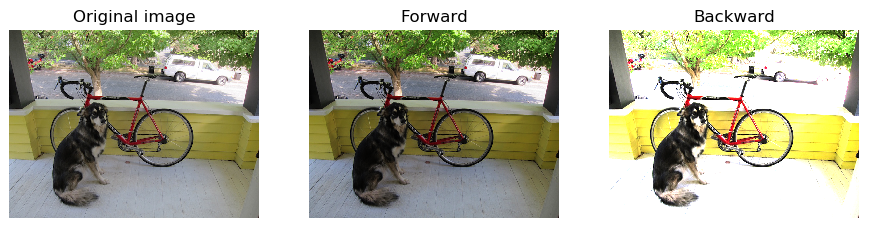
\includegraphics[scale=0.5]{./images/activation_elu}
 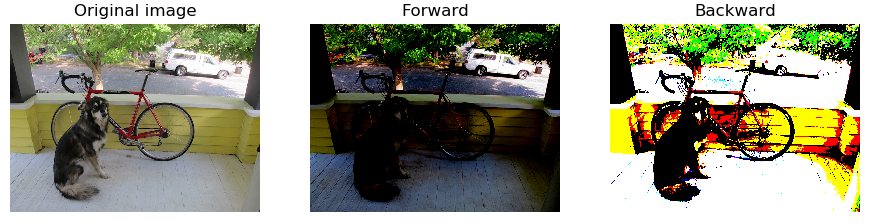
\includegraphics[scale=0.5]{./images/activation_relu.png}
 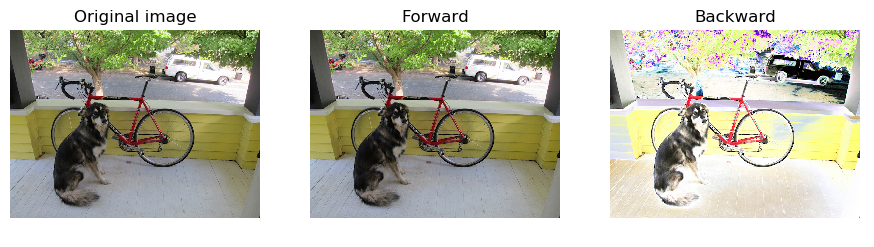
\includegraphics[scale=0.5]{./images/activation_logistic.png}
 \caption{\it Activation functions applied on test image. From top to bottom: Elu, Relu and Logistic.}
 \label{fig:activations}
\end{figure}

The most used activation functions is undoubtedly the {\tt ReLU} activation (Rectified Linear Unit.) \cite{Relu}. Its main advantages are:

\begin{itemize}
 \setlength\itemsep{-0.2em}
 \item Sparsity: a sparse representation of data is exponentially more efficient in comparison of a dense one.
 \item Vanish Gradient Reduction, since the derivatives does not vanishes during Deeper backpropagation.
 \item Easy and fast computation of both forward and backward.
\end{itemize}

\subsection*{Cost Function}

A Deep Learning model is trained by minimizing a Cost Function, or, in other words, during training we want to adjust the parameters of the network in order to modify its output, which in turns, will be closer to the desired result. 
Therefore, it is important to define what we consider the error function of the model.
There are many kinds of loss functions, and none of them is able to work with every kind of data; moreover, there are no particular reasons to prefer a loss function over another one, given that they are both adapt to handle the output of the problem under analysis. 
One important property is the differentiability of those error functions, since they will be the starting point of chain rule for derivatives used in {\it Error Backpropagation}.
Broadly speaking, loss functions can be separated into two categories: classification losses and regression losses. In the first case we want to predict a finite number of categorical values (classes), while in the second case the prediction is performed over a series of continuos values.
The most common cost functions for Super Resolution are {\it Mean Squared Error} (MSE) and {\it Mean Absolute Error} (MAE), also called L2 loss and L1 loss. 
The former is defined as: 

\begin{equation}
 MSE = \frac{1}{N} \sum_{i=1}^{N} (y_i - t_i)^2
\end{equation}

where $\bm{y}$ is the output vector of the model, $\bm{t}$ is the desired results and $N$ is the dimension of the output.
It is one of the most used loss function for different task, not only because is really simple, but also because it reaches good performances.
Notice that minimizing the MSE naturally maximize the PSNR score define in previous chapter.

In MAE we replace the squared error with the absolute difference:

\begin{equation}
 MAE = \frac{1}{N} \sum_{i=1}^{N} |y_i - t_i|
\end{equation}

Both models used in this work have been trained using the L1 loss function. 

\section{Timing}

I tested {\tt Byron} performances on single layers through its python wrap {\tt Pyron} against the popular deep learning framework {\tt Tensorflow} on CPU.
I measured the forward and backward times on 30 repetitions, scanning over the parameters of the different layers as fuctions of the number of threads, for the most important layers in image processing applications: Convolutional, Max-Pool and Pixel-shuffle layer.
The number of threads indicates the level of parallelization involved during computations.
The inputs are randomly generated tensors of dimensions $16 \times 512 \times 512 \times 3$ which should resemble a batch of images. 
The content of said images does not really matter, since we are only interested in measuring the processing times.
For the first case, the results for {\it forward} and {\it backward} functions are summarized in figure \ref{fig:time-conv}:

\begin{figure}[H]
\centering
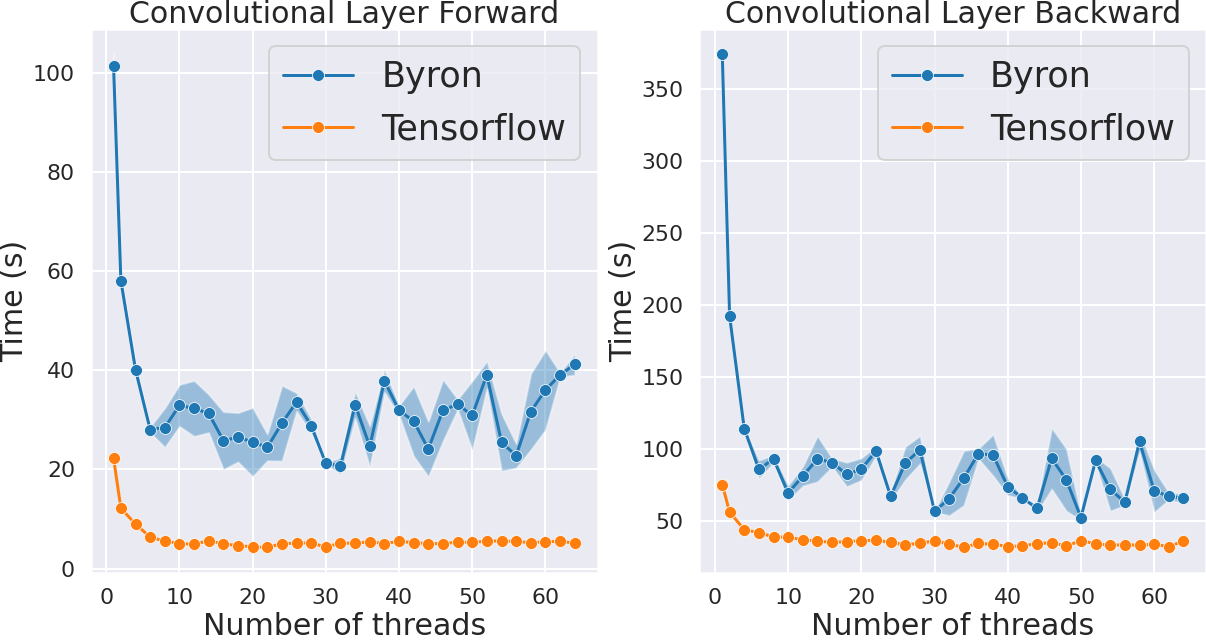
\includegraphics[scale=0.3]{./images/convolutional_timing_3_1.png}
\caption{\it Comparisons between time to perform forward (left) and backward (right) for Convolutional Layer in Byron and Tensorflow on a 4D tensor of size $16 \times 512 \times 512 \times 3$ for size 3, stride 1 and 100 filters.}
\label{fig:time-conv}
\end{figure}

As expected, the performances improve with higher numbers of threads, however this behaviour last for less than 10, after which the times remain constant for both implementations.
In particular, for {\tt Byron}, the algorithm's time seems to be really unstable with higher number of opened threads. 
Nonetheless, the CPU times of {\tt Tensorflow} are consistently better that {\tt Byron}.
Those considerations highlight that there may be problems in threads management during the operations in {\tt Byron}, which do not influence the outputs, but greatly deteriorate timing performances.
If we move to a bigger stride value, like 2, the results change as shown in \ref{fig:time-conv-3-2}. 
In particular, the trends become slighlty more stable a not far from what we are expecting.
The conditions $size=3$ and $stride=1$ are also the condition for the {\it Winograd Algorithm}: this can reduce the range of code to check to find the sources of times instability.
Another considerations come from the fact that passing from $stride=1$ to $stride=2$ in both axis, reduce the number of operations of a factor 4, which means, at least, that the single thread performances should reduce the time cost of 4 time.
In {\tt Byron} forward though, the time reduces to roughly $40\%$, while in {\tt Tensorflow} the speed up seems consistent with that consideration.

\begin{figure}[H]
\centering
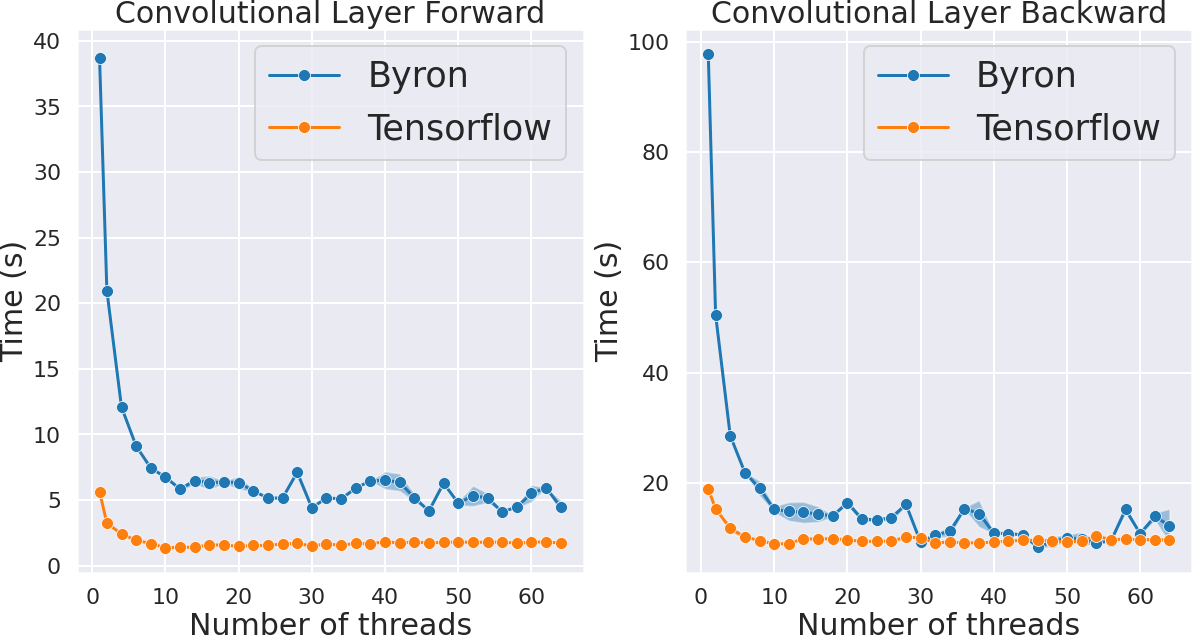
\includegraphics[scale=0.3]{./images/convolutional_timing_3_2.png}
\caption{\it Comparisons between time to perform forward (left) and backward (right) for Convolutional Layer in Byron and Tensorflow on a 4D tensor of size $16 \times 512 \times 512 \times 3$ for size 3, stride 2 and 100 filters.}
\label{fig:time-conv-3-2}
\end{figure}

The second case taken into account is MaxPool Layer and the results are summarized in figure \ref{fig:time-max-3}:

\begin{figure}[H]
\centering
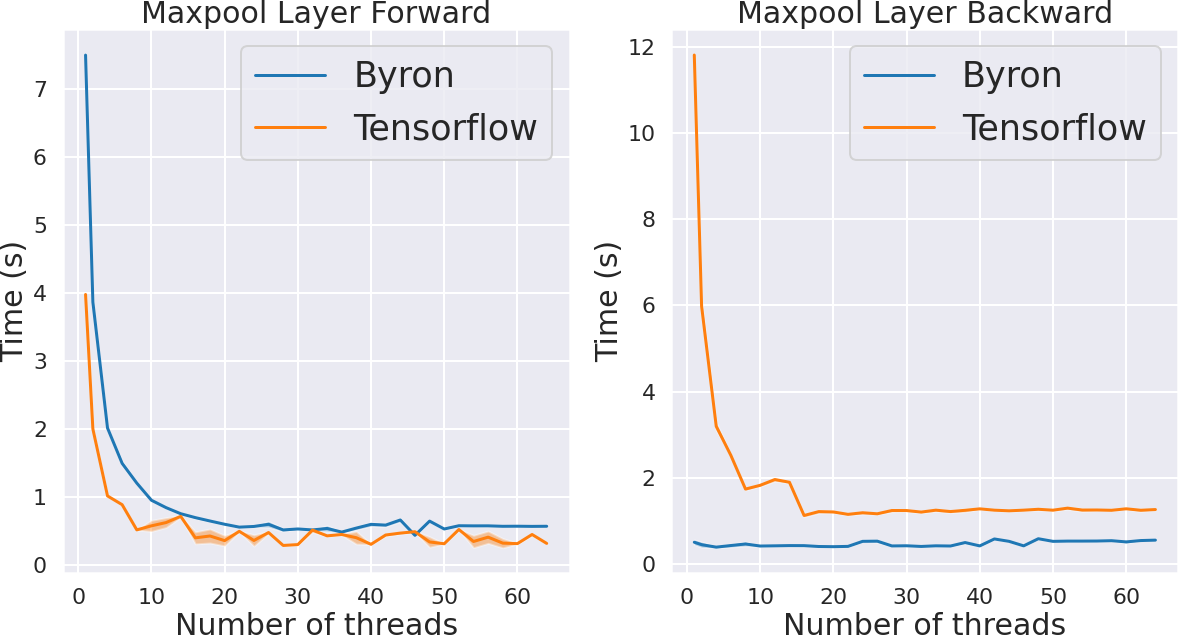
\includegraphics[scale=0.29]{./images/maxpool_timing_3.png}
\caption{\it Comparisons between times to perform forward (left) and backward (right) for Maxpool Layer in Byron and Tensorflow on a 4D tensor of size $16 \time 512 \times 512 \times 3$ for size 3 and stride 1.}
\label{fig:time-max-3}
\end{figure}

In this case, the results seems to show comparable times for {\tt Byron} and {\tt Tensorflow} for the forward function and a faster implementation for the backward function.
Again, the time gained by adding more threads does not improve much after a certain number: this can also be due to the dimensions of the input not being large enough to justify opening such an high numbers of parallel operations. 
All-in all, this implementation seems to be performing as expected.
Moreover, using an higher kernel size seems to favour {\tt Byron} over {\tt Tensorflow}, as shown in figure \ref{fig:time-max-30}

\begin{figure}[H]
\centering
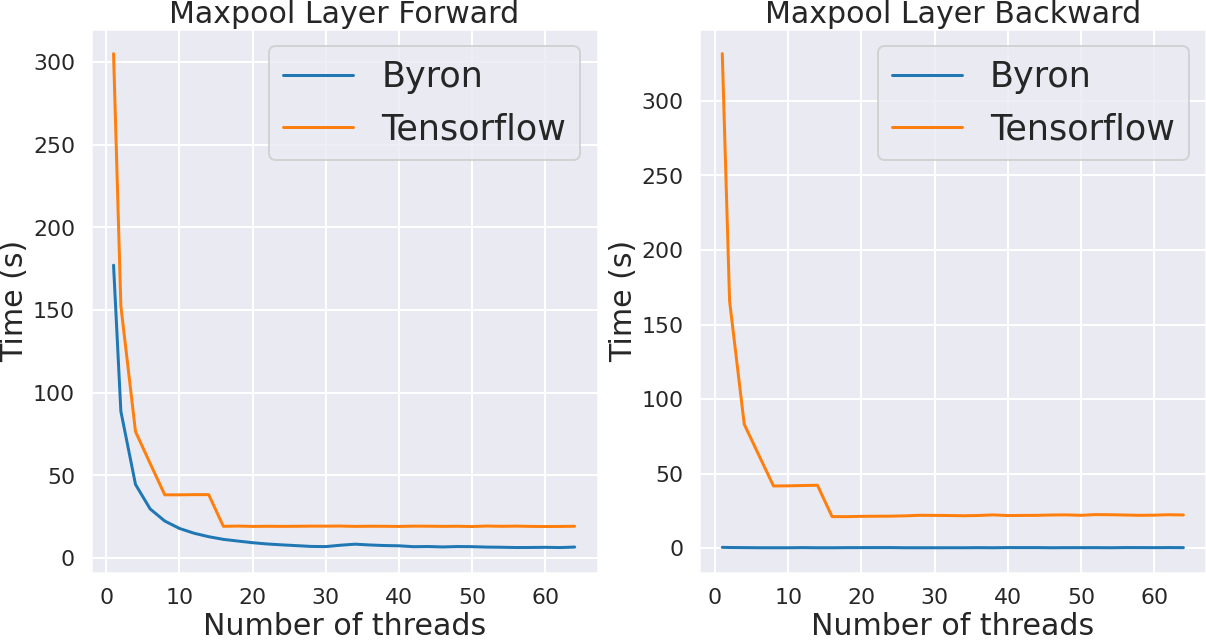
\includegraphics[scale=0.29]{./images/maxpool_timing_30.png}
\caption{\it Comparisons between times to perform forward (left) and backward (right) for Maxpool Layer in Byron and Tensorflow on a 4D tensor of size $16 \time 512 \times 512 \times 3$ for size 30 and stride 1.}
\label{fig:time-max-30}
\end{figure}

This may indicates that the higher the numbers of operations, the higher is the advantage gained with {\tt Byron}.
In our implementation of Maxpool Layer, during the forward function we store the indexes needed for the backward operation: in this way we lose a bit of time during the forward pass, however the backward become just a single {\tt for loop} on the array of indexes. Most likely, {\tt Tensorflow} opted for a different implementation, given the results.

The third layer taken into consideration is the Pixel Shuffle, in particular I considered a scale factor of 6 with an input tensor of dimension $16 \times 512 \times 512 \times 108$. 
The singular number of input channels has been chosen to be compatible with the re-scaling performed by the pixel-shuffle operation.
The {\tt Tensorflow} implementation of Pixel shuffle seems to behave very differently from previous cases: indeed it does not scale at all with the number of threads, and times remain very similar from 1 to 64 parallel sections.
Again, the single thread performances favour {\tt Tensorflow} over {\tt Byron}: although in the forward function {\tt Byron} speed ups quickly with the higher number of threads.  
I would like to point out that even if the two operations of forward and backward are very similar, being only re-arrengement of the same number of pixels, the latter seems to be faster in both implementations.
The other scale factor and input shapes tested does not show any different behaviour from the ones described in this case.

\begin{figure}[H]
\centering
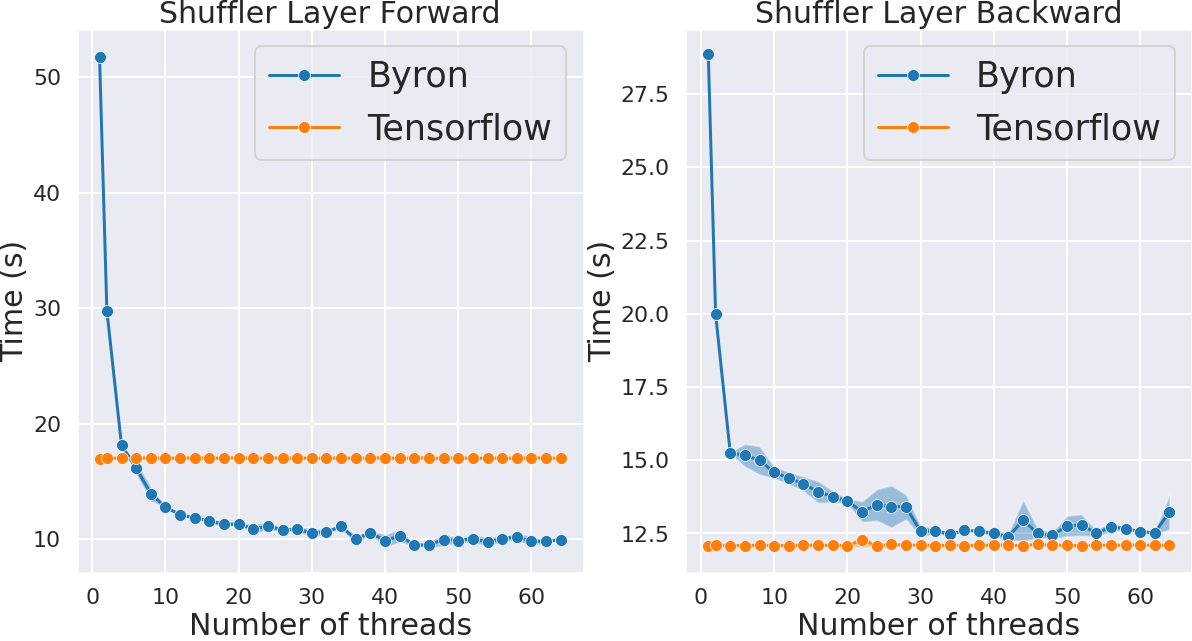
\includegraphics[scale=0.3]{./images/shuffler_timing_6.png}
\caption{\it Comparisons between times to perform forward (left) and backward (right) for Shuffler Layer in Byron and Tensorflow on a 4D tensor of size $16 \time 512 \times 512 \times 108$ for scale 6}
\label{fig:time-shuf-6}
\end{figure}

\chapter{Datasets and Methodology}

\section{Models}

As already described in previous chapters, the high level of modularity provided by \texttt{Byron} and \texttt{NumPyNet} allows to use different kind of models for many different purposes. \\ The two models chosen for super-resolution are {\tt EDSR}, used to performs a x2 upsample, and {\tt WDSR}, used to perform a x4 upsample. 
They are the winners of the {\it NTIRE} challenge (New Trends in Image Restoration and Enhancement) respectively for the year 2017 and 2018 and the model structure and weights are publicly available at their official github repositories; \href{https://github.com/thstkdgus35/EDSR-PyTorch}{EDSR} and \href{https://github.com/JiahuiYu/wdsr_ntire2018}{WDSR}.

\subsection*{EDSR}

{\tt EDSR} (Enhanced Deep Super-Resolution) \cite{edsr} is the first model considered and ported in {\tt Byron}. 
It is a Deep Neural Network specialized in Single Image Super Resolution (SISR) which won the NTIRE challege in 2017.
Its structure is based on previous famous models in image analysis application, namely {\tt SRResNet} and, consequently, {\tt ResNet}. 
For this reason, the base unit of {\tt EDSR} is the {\it residual block}, which makes extensive use of {\it residual connections}, described in the previous chapter.
The major improvements from older models come from removal of batch-normalization between convolutional layers inside {\it residual blocks}: indeed the authors proved experimentally that normalization of the features reduces performances substantially, by getting rid of range flexibility \cite{edsr}. 
Moreover, every Batch-Norm layer contains the same amount of weights as the convolutional layer preceeding it, therefore removing them saves approximately 40\% of memory usage during training and this allows the construction of larger models.
On the other hand, they also showed that deepening the model above a certain level would make the training procedure numerically unstable: the authors solved this issue by adopting a residual scaling with factor $0.1$ in shortcut connections. 
 
The structure of the model is summarize in figure \ref{fig:edsr-structure}.
The model used in this work is called {\it EDSR\_x2} by the authors and is composed by 32 {\it residual block}, each in turn is composed by: 

\begin{itemize}
 \setlength\itemsep{-0.2em}
 \item A convolutional layer with 256 filters
 \item An activation layer with a ReLU function
 \item A convolutional Layer with 256 filters
 \item A linear combination pixel-by-pixel with the input of the residual block with weight respectively 0.1 and 1 (shortcut connection's $\alpha$ and $\beta$)
\end{itemize}

\begin{figure}[H]
 \centering
 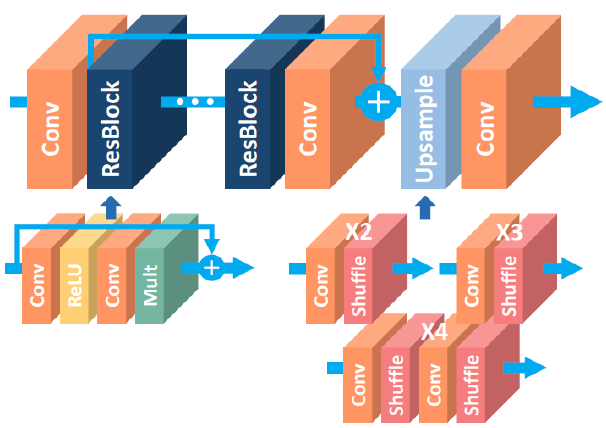
\includegraphics[scale=0.4]{./images/edsr_structure.png}
 \caption{\it architecture of the single scale SR Network (EDSR)}
 \label{fig:edsr-structure}
\end{figure}

The last part of the network is composed by a shortcut connection which performs a linear combination of the initial input with the output of the 32 residual block and by the up-sampling block:

\begin{itemize}
 \setlength\itemsep{-0.2em}
 \item A convolutional layer with 1024 filters 
 \item A pixel-shuffle with a scale factor $r=2$  
 \item A convolutional layer with 3 filter (the final output.)
\end{itemize}

In total, {\tt EDSR} has more than 40 millions of parameters, summarized in table \ref{tab:edsr-weights}

\begin{table}[H]
\begin{center}
\setlength{\tabcolsep}{14pt}
\begin{tabular}{|l l l l|}
 \hline
 Layer & Channels in/out & Filters Dim. & Parameters \\
 \hline
 Conv. Input       & 3 / 256     & 3x3 & 6912\\ [0.3cm]
 Res. Block        & 256 / 256   & 3x3 & 1179648\\[0.3cm]
 Conv. Pre Short.  & 256 / 256   & 3x3 & 589824\\[0.3cm]
 Conv. Pre-Shuffle & 256 / 1024  & 3x3 & 2359296 \\[0.3cm]
 Conv. Output      & 256 / 3     & 3x3 & 6912\\
 \hline
\end{tabular}
\end{center}
\label{tab:edsr-weights}
\caption{\it Table of parameters for the different sections of EDSR.}
\end{table}

The "heaviest" part of the model is clearly the Residual Blocks section, which alone contains more that 37 millions of parameters.

For training they used $48 \times 48$ RGB patches from LR images (from DIV2K) with the corresponding HR patches, augmenting the training data with random horizontal flips and 90° rotations. 
The optimizer is the ADAM \cite{adam} and the loss function is the L1: even if the L2 naturally maximize the PSNR (which is the only metrics evaluated in the challenge), they found that L1 loss provided a better convergence.

\subsection*{WDSR}

The second model considered in this study and implemented in {\tt Byron} is called Wide Deep Super Resolution (WDSR) \cite{wdsr} and it is the winner of the NTIRE challenge 2018. 

The model used in ths work is called {\tt WDSR\_x4\_A} and it is composed by 32 residual blocks, similarly to {\tt EDSR}, the difference is that they are much lighter in this case, indeed a residual block is composed by:

\begin{itemize}
 \setlength\itemsep{-0.2em}
 \item Convolutional layer with 192 filters 
 \item Activation layer with ReLU function 
 \item Convolutional Layer with 32 filters
 \item Shortcut connection with $\alpha = \beta = 1$
\end{itemize}

In their work, the authors designed the network to study the importance of {\it wide features} before ReLU activations. Indeed they slim the features of residual identity mapping pathway while expanding the features before activation.
From this simple idea they claim {\tt WDSR-A} is extremely effective for improving accuracy of single image super-resolution when the scale factor is between 2 and 4, but the performance drops quickly after this threshold.

Another important step is the introduction of weight normalization over batch normalization (BN) which does not introduce the troubles of BN while speeding up the convergence of Deep Neural Networks, by allowing the usage of higher learning rates \cite{wdsr}.

Further improvements can be found in the structure of the network as shown in figure \ref{fig:edsr-wdsr-structure}: they simplify the network architecture by removing redundant Convolution pre-shuffling. 
Thus, they modify the structure by introducing a single convolutional layer with size $5  \times 5$ that works directly on the input, extracting the low frequency features of the sample. 
Those modifications result in less parameters, without affecting the accuracy.

\begin{figure}[H]
 \centering
 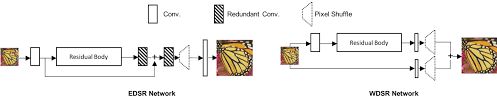
\includegraphics[scale=0.6]{./images/edsr_wdsr_structure.png}
 \caption{\it comparisons between {\tt EDSR} architecture on the left and {\tt WDSR} architecture on the right}
 \label{fig:edsr-wdsr-structure}
\end{figure}

A summary of the model's sections along with the numbers of weights they contains can be found in table \ref{tab:wdsr-weights}: 

\begin{table}[H]
\begin{center}
\setlength{\tabcolsep}{14pt}
\begin{tabular}{|l l l l|}
 \hline
 Layer & Channels in/out & Filters Dim. & Parameters \\
 \hline
 Conv. Input           & 3 / 32   & 3x3 & 864  \\[0.3cm]
 Res. Block Conv. (1)  & 32 / 192 & 3x3 & 55296\\[0.3cm]
 Res. Block Conv. (2)  & 192 / 32 & 3x3 & 55296\\[0.3CM]
 Conv. Pre Shuffle (1) & 32 / 48  & 3x3 & 13824\\[0.3cm]
 Conv. Pre-Shuffle (2) & 3 / 48   & 5x5 & 38400\\
 \hline
\end{tabular}
\end{center}
\label{tab:wdsr-weights}
\caption{\it Table of parameters for the different sections of WDSR.}
\end{table}

In total, {\tt WDSR\_A} is composed by more that 3 millions parameters, still 10 time less than {\tt EDSR} while reaching similar results if compared on the same categories.
The lesser amount of weights not only decreases memory usage during both test and training, but also greatly increse computational performance: indeed a single forward of {\tt WDSR} is more than 10 times faster than {\tt EDSR}.
The training dataset is composed by $96 \times 96$ patches from every images of the training section of the DIV2K dataset. Again, the data are augmented with random horizontal flips and rotations and the optmizer is ADAM \cite{adam} minimizing the L1 loss functions.

\newpage

\section{Train Dataset: DIV2K}

The training set is a general purpose dataset called DIV2K \cite{DIV2K} and it has been employed to train and validate {\tt EDSR} and {\tt WDSR} for the {\it NTIRE} competition ({\it New Trends in Image Restoration and Enhancement}).

The dataset is composed by 1000 2K RGB images with a large diversity of contents, divided into:

\begin{itemize}
 \setlength\itemsep{-0.2em}
 \item {\bf Training set}: 800 HR images and 800 LR images obtained from the HR ones using different downscaling factor (2x, 3x, 4x) and different degrading factors.
 \item {\bf Validation set}: 100 HR images and 100 LR images used as a test set to evaluate the models by the competitors.
 \item {\bf Test set}: 100 LR images for which an HR version is made available only at the end of the competition. This is used by the competitors to test the models and for their final evaluation.
\end{itemize}

A qualitative proof of the results obtainable from the two models are shown in pictures \ref{fig:sky}, \ref{fig:city} and \ref{fig:windows}.

\begin{figure}[H]
  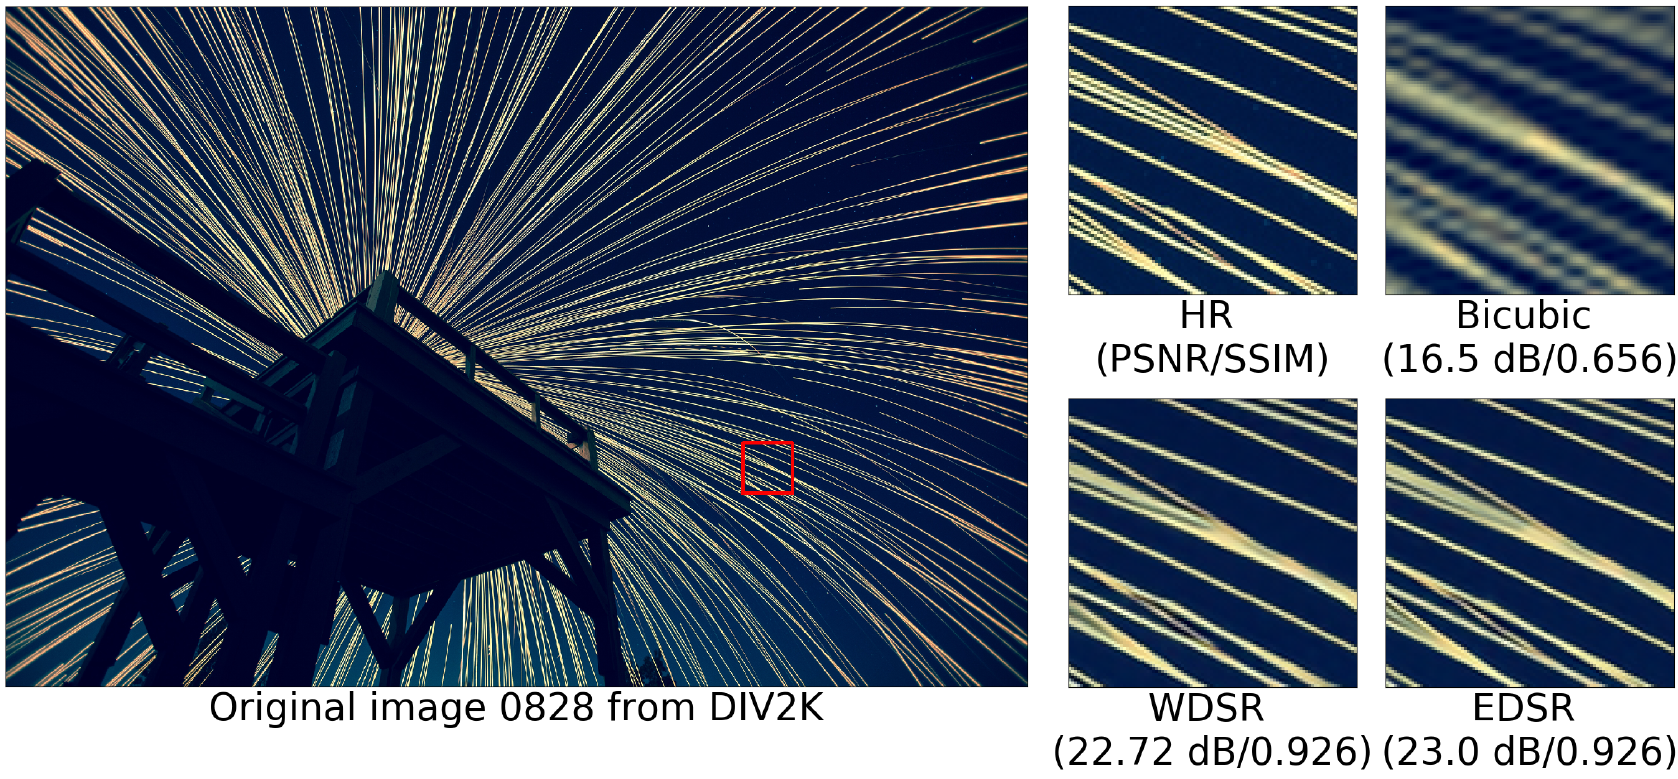
\includegraphics[scale=0.5]{images/sr_res1.png}
    \caption{\it Super Resolution visual example extracted from the DIV2K validation set. The quality score in terms of PSNR and SSIM are compared between a standard bi-cubic up-sampling and the EDSR and WDSR models.}
  \label{fig:sky}
\end{figure}

\begin{figure}[H]
  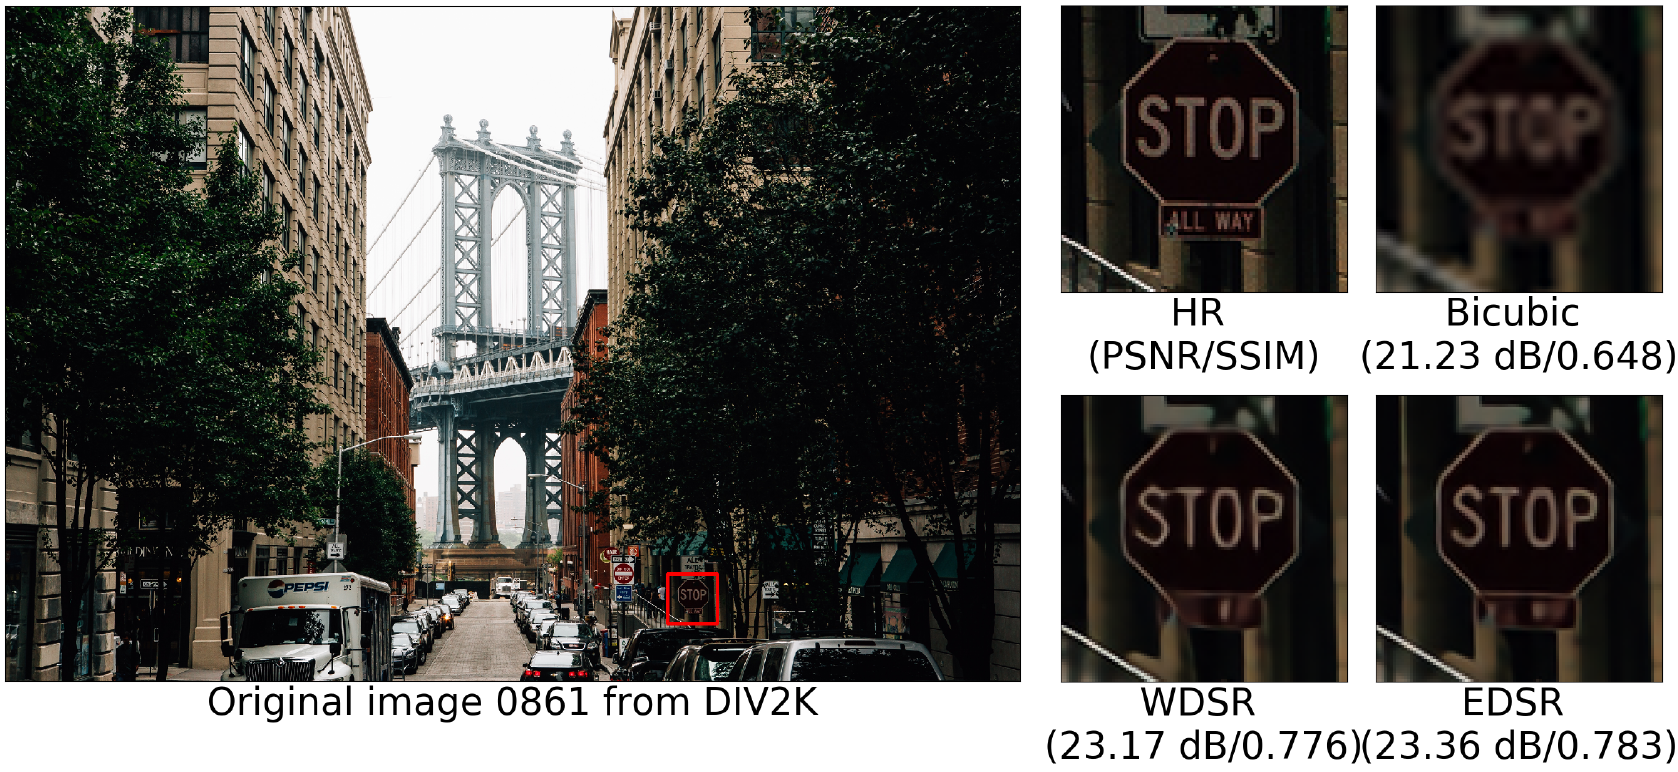
\includegraphics[scale=0.5]{images/sr_res2.png}
    \caption{\it Super Resolution visual example extracted from the DIV2K validation set. The quality score in terms of PSNR and SSIM are compared between a standard bi-cubic up-sampling and the EDSR and WDSR models.}
  \label{fig:city}
\end{figure}

\begin{figure}[H]
  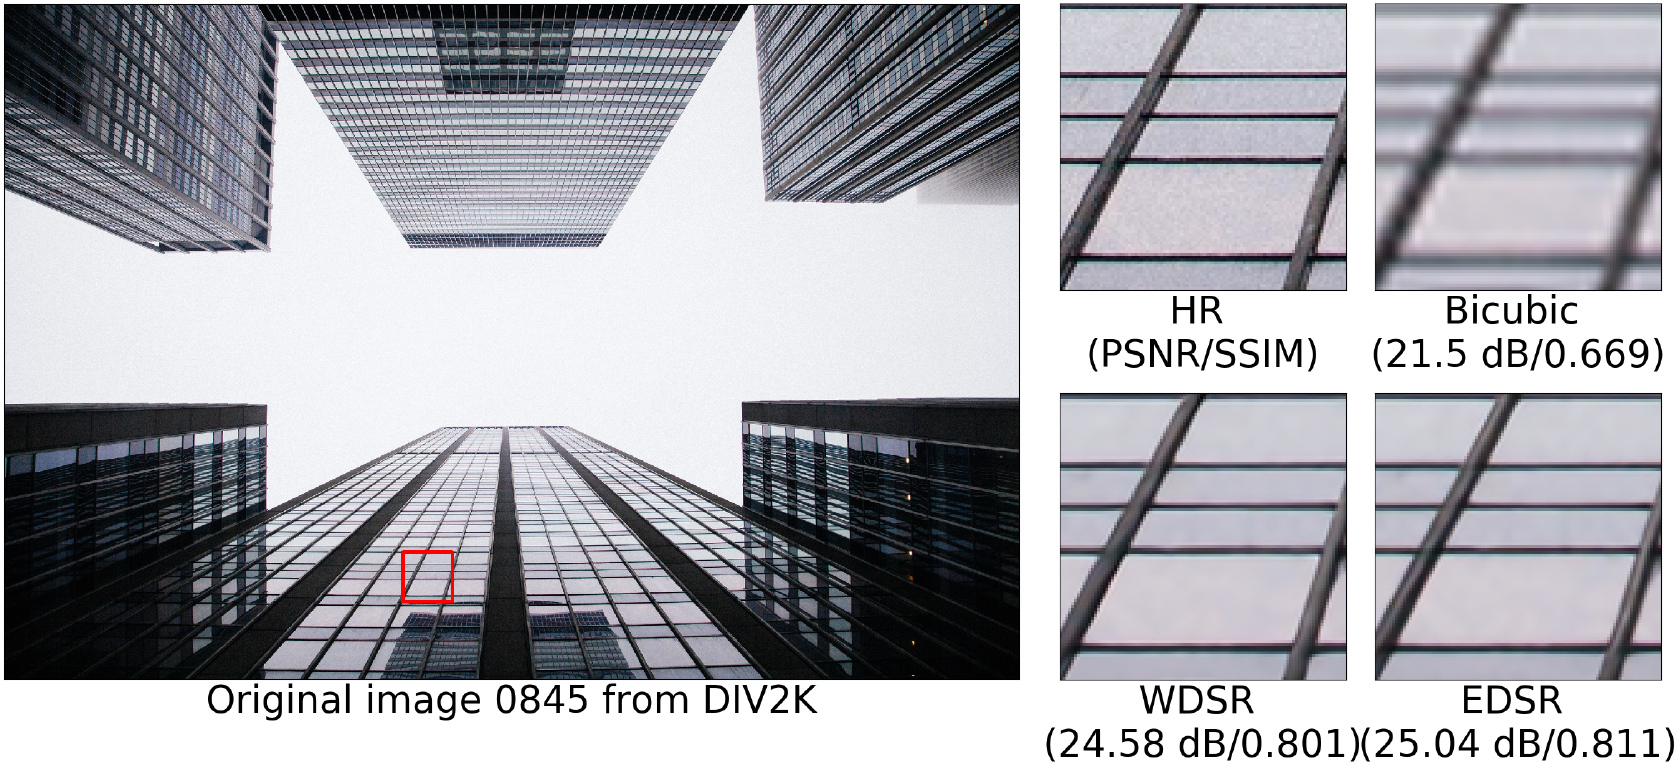
\includegraphics[scale=0.5]{images/sr_res3.png}
  \caption{\it Super Resolution visual example extracted from the DIV2K validation set. The quality score in terms of PSNR and SSIM are compared between a standard bi-cubic up-sampling and the EDSR and WDSR models.}
  \label{fig:windows}
\end{figure}

As can be seen in those pictures, the models have learned how to interpolate the complex line shapes and different kind of textures better than the bicubic algorithm.
Given the great heterogeneity of contents inside the dataset, after the training phase the models are able to reconstruct a huge amount of distict shapes and textures. For this reasons we decided to test the performances of {\tt WDSR} and {\tt EDSR} on a set of NMR data. 

\section{NMR Dataset}

To test the model on NMR images, we used a series of 5 patients weighted $T_1$ and $T_2$ sampled with a spatial frequency of $1mm \times 1mm \times 1mm$ for each direction ($x, y, z$), with a resolution of $256 \times 256$ for a total of 176 slices. For reference, in figure \ref{fig:orig_ref} are shown three different slices for the same patient at HR:

\begin{figure}[H]
 \centering
 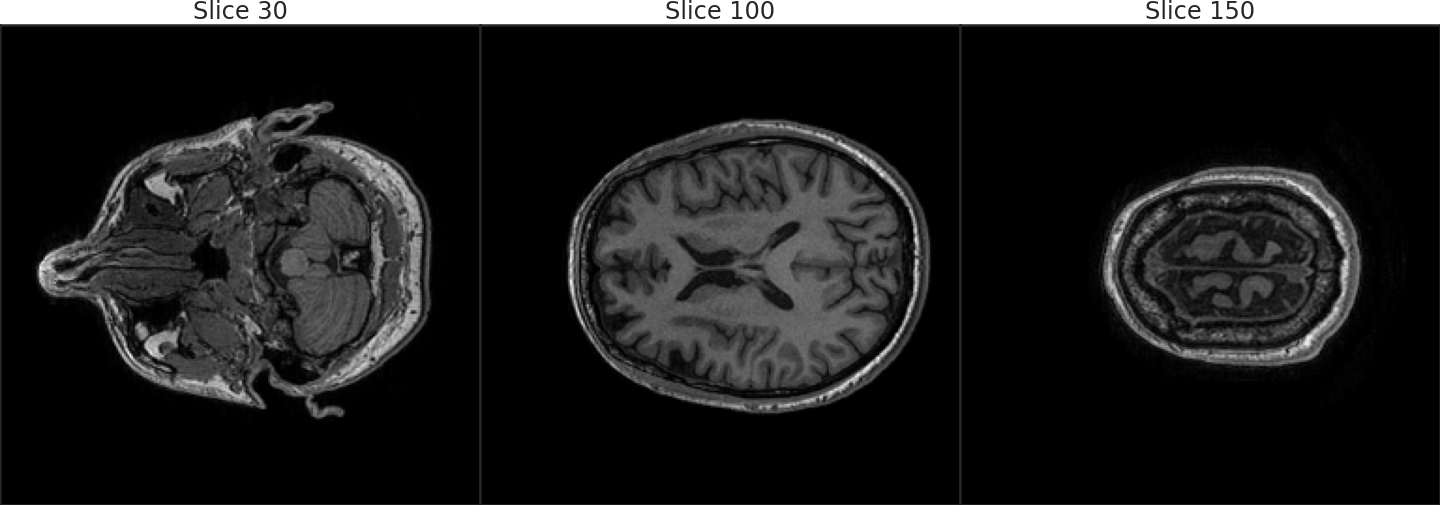
\includegraphics[scale=0.31]{./images/orig_slice_comp.png}
 \caption{\it HR $256 \times 256$ original image at three different stages of depth: (left) slice 30 where still a lot of information about the brain is hidden, (center) slice 100 which is a central slice where most of the information is stored, (right) slice 150 which starts the less informative area of the brain.}
 \label{fig:orig_ref}
\end{figure}

The HR images (which will also be called {\it originals}) are convoluted with a gaussian kernel of size 3, stride 1 and standard deviation 1 with the function \texttt{cv2.GaussianBlur} of the library \texttt{OpenCV}. 
Then, they have been  downsampled with the bicubic algorithm by two different scale factors, namely $\times 2$ and $\times 4$, with the function \texttt{resize}, also available from {\texttt OpenCV}, obtaining two distinct sets of LR images for every subject and for every weight, respectively of sizes $128 \times 128 \times 176$ and $64 \times 64 \times 176$.
The gaussian blurring has been done to better resemble a LR data-acquisition, as if the images were obtained at low resolution directly and not coming from a downsampling.
In figure \ref{fig:inp2} is shown an example of the images obtained by this procedure for a downscale factor of 2:

\begin{figure}[H]
 \centering
 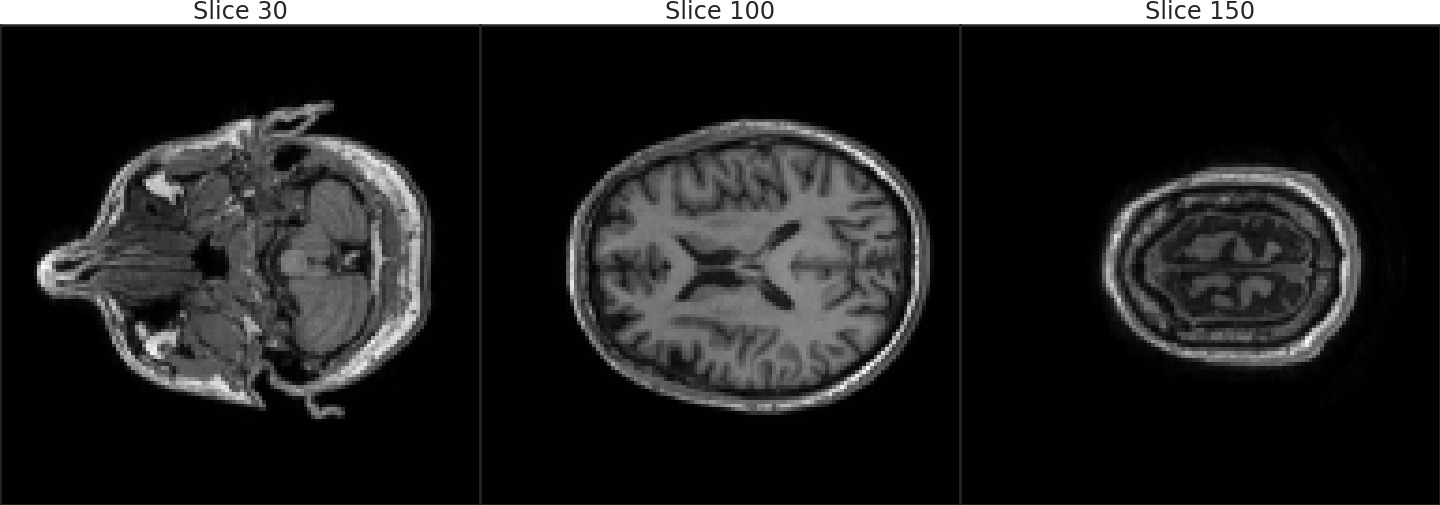
\includegraphics[scale=0.3]{images/inp2_slice_comp.png}
 \caption{\it $128 \times 128$ LR version of the same slices shown for the HR case.}
 \label{fig:inp2}
\end{figure}

In figure \ref{fig:inp4} is shown an example of the images obtained by this procedure for a downscale factor of 4:

\begin{figure}[H]
 \centering
 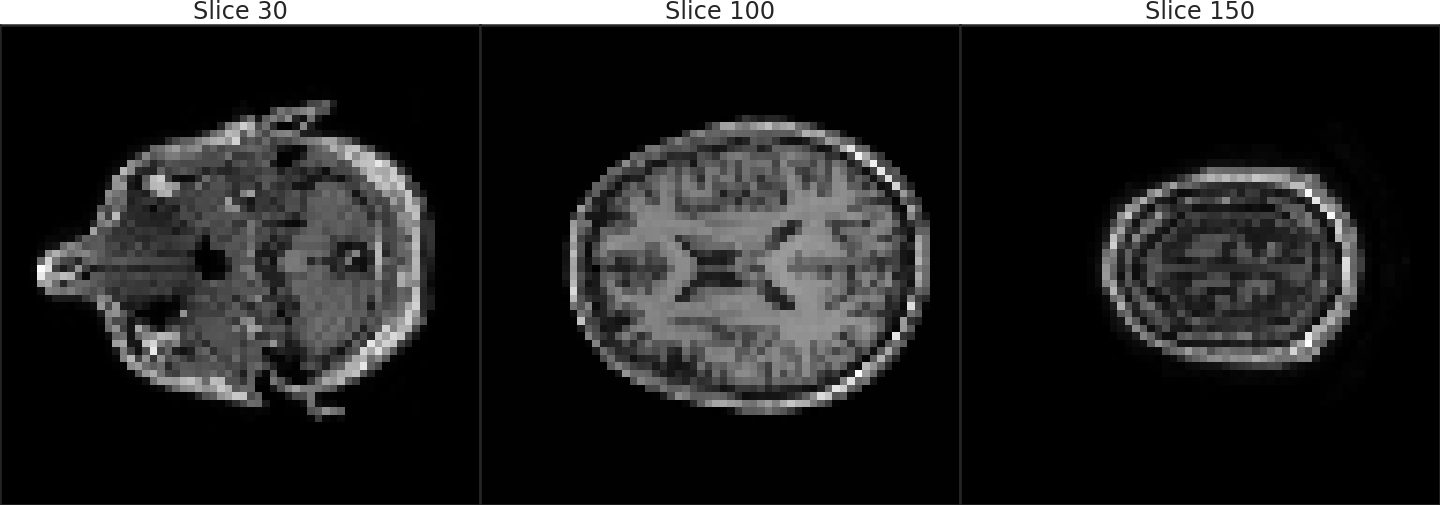
\includegraphics[scale=0.3]{images/inp4_slice_comp.png}
 \caption{\it $64 \times 64$ LR version of the same slices shown for the HR case.}
 \label{fig:inp4}
\end{figure}

The LR images are used as input for {\tt EDSR}, {\tt WDSR} and the bicubic algorithm which re-upsample them respectively by factors $\times 2$, $\times 4$ and both, trying to recostruct an image as close as possible to the original one.
As a further analysis, I decided to investigate how different input conditions influence the results for the three methods. 
In particular how an angle of rotation for the LR images can impact the final re-upsample: indeed this changes the orientation of lines, shapes, and textures, which can affect the reconstruction.
Nonetheless it can give an important insight on the level of invariance of the two models and on the {\it explainability} of the results. 

I divided the full angle into 20 sections, separated by a step of $18$°. In figure \ref{fig:rotations} is shown an example of the kind of inputs fed to the models:

\begin{figure}[H]
 \centering
 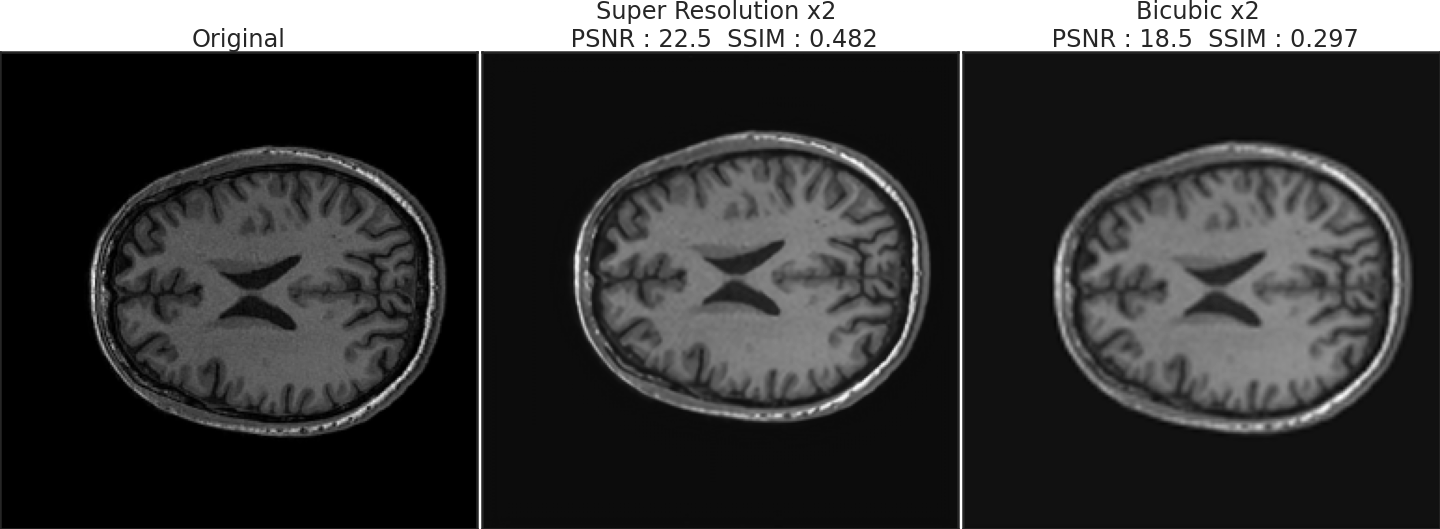
\includegraphics[scale=0.3]{images/rotations.png}
 \caption{\it Three of the 20 rotation angles used as input for Super Resolution models and Bicubic. (left) reference angle of 0 degree, (centre) angle step of 18 degree, (right) large rotation of 108° respect to the reference. }
 \label{fig:rotations}
\end{figure}

The recostruction are compared with the original images using PSNR and SSIM values for every patient, weight, channel, scale factor and angle of rotation. 
As stated before, the NMR slices are 1-channeled gray-scale image while the SR models work on RGB image: this is solved by adding an artificial depth concatenating the same slice 3 times. 
The dataset of original HR images is publicly available from \href{http://insight-journal.org/midas/collection/view/190}{NAMIC} \cite{dataset}. 

\chapter{Results}

In the following chapter I am going to report quantitative and qualitative results for the different analysis carried out during the work.
I describe the quantitative results obtained by the different methods evaluated by means of PSNR, SSIM score and by a qualitative visual analisys.
At the end of the chapter I will summarize the results and provides possible continuations for future analysis.  

\section{Upsample Comparisons}

The {\tt EDSR} model is used to upsample the images by a $\times 2$ factor so that the single slice is super-resolved from a $128 \times 128$ to a $256 \times 256$ spatial resolution. 
The {\tt WDSR} model instead, is used to upsample the images by a $\times 4$ factor so that the single slice is super-resolved from a $64 \times 64$ to a $256 \times 256$ spatial resolution. 

I decided to separate the analysis for the three output channels of the super-resolution since it can highlight particular behaviours. 
Moreover, the two kinds of MRI, T1-weighted and T2-weighted, will also be evaluated separately, because it can give a useful insight on what the models are able to ``see''.  
In figure \ref{fig:edsr-score-slide-t1} are shown the average trends for PSNR and SSIM score for the three channels (Red, Green, Blue lines) and for the bicubic algorithm (Yellow lines), of cases weighted T1.
They are averaged for all patients and angle of rotations.
It is clear that there is a difference between the three outputs for the super resolution: namely there is a vertical shift in the trends passing from Red to Green and from Green to Blue, the latter being the best performer.
Moreover, the ``best'' channel for {\tt EDSR} outperforms consinstently the bicubic algorithm, and the second best outperforms the bicubic algorithm in the most informative section of the images. 

\begin{figure}[H]
  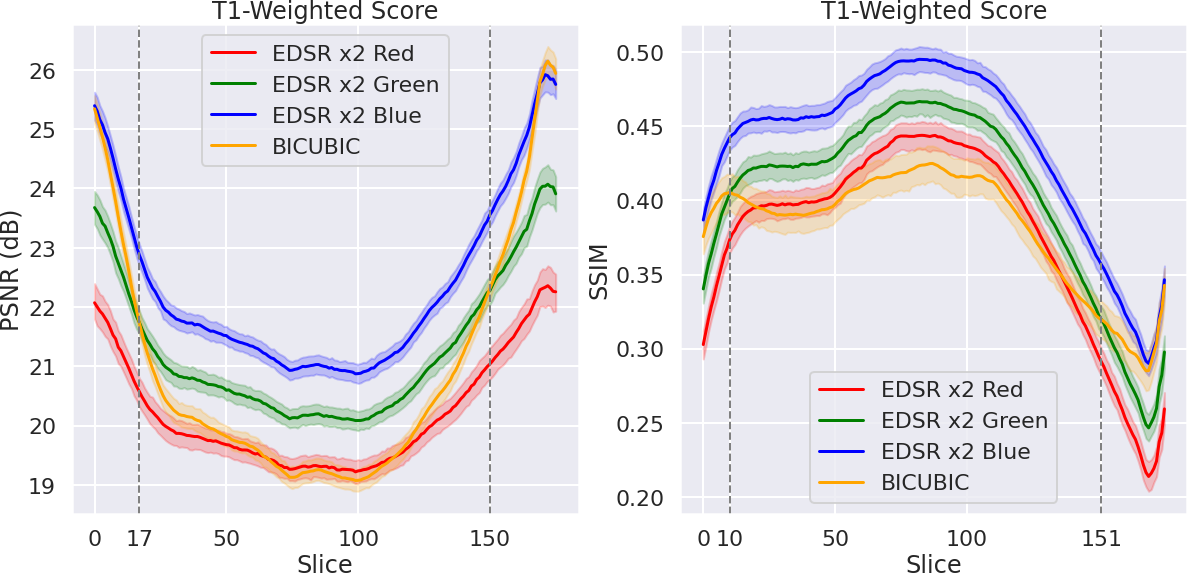
\includegraphics[scale=0.37]{./images/EDSR_score_slide_t1_all.png}
  \caption{\it Average trends of PSNR (left) and SSIM (right) for the three channels (Red, Blue, Green lines) of the Super Resolution EDSR model compared with the bicubic algorithm scores (Yellow) as functions of the slices. The average is performed for every patients and for every rotation,  cosidering only T1 weighted NMR. The dotted lines highlights the slices where the bicubic and super-resolution green channel performances intersect.}
  \label{fig:edsr-score-slide-t1}
\end{figure}

In figure \ref{fig:edsr-upscale} is shown an example on the kind of reconstruction the two methods are able to achieve on a significant slice: 

\begin{figure}[H]
 \centering
 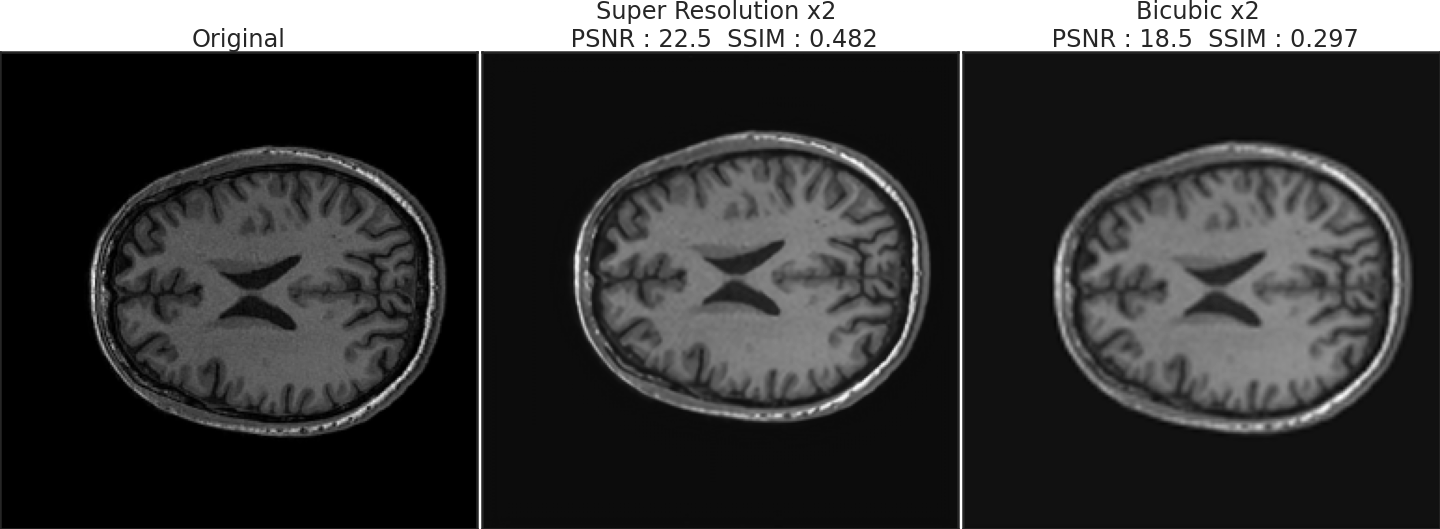
\includegraphics[scale=0.3]{./images/edsr-comp-images.png}
 \caption{\it (left) original image, (center) reconstruction performed with {\tt EDSR} blue channel, (right) reconstruction using the bicubic method. The input in this case is not rotated.}
 \label{fig:edsr-upscale}
\end{figure}

In the {\tt EDSR} reconstruction there seems to be generally less noise, both around edges and more so in the gray area of the brain. 
\\
On the other hand, the results for T2-weighted NMRs are a bit different, indeed figure \ref{fig:edsr-score-slide-t2} highlights how the performances of EDSR are relatively worse compared with the previous case.

\begin{figure}[H]
 \centering
 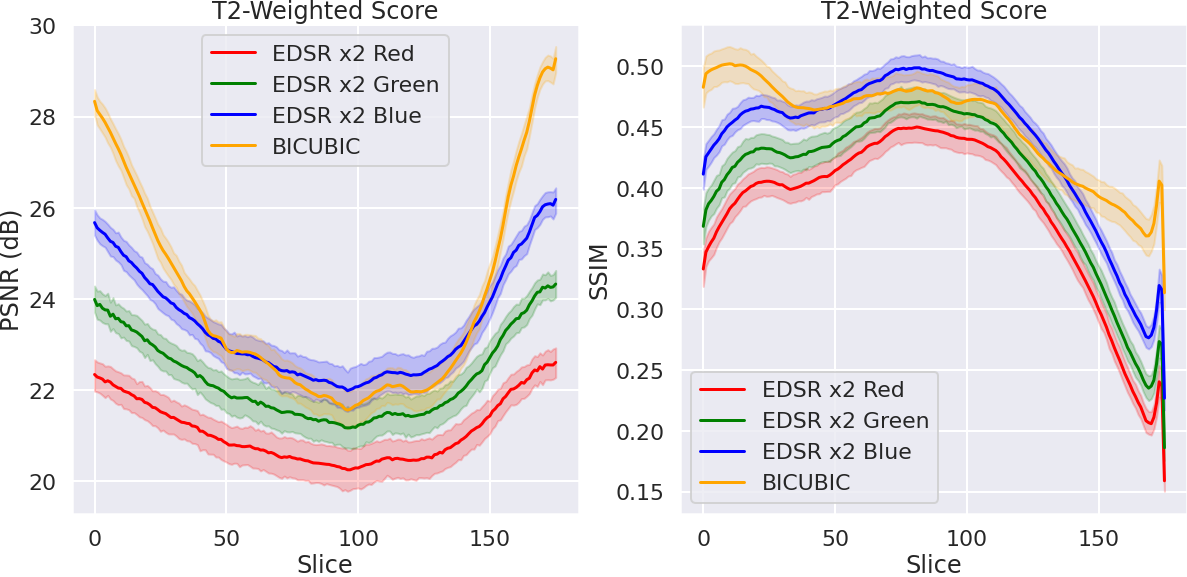
\includegraphics[scale=0.3]{./images/EDSR_score_slide_t2_all.png}
 \caption{\it Average trends of PSNR (left) and SSIM (right) for the three channels (Red, Blue, Green lines) of the super-resolution EDSR model compared with the bicubic algorithm scores (Yellow) as functions of the slices. The average is performed for every patients and for every rotation,  considering only T2-weighted NMRs. In this case the bicubic seems to perform better, a part from the central section of the slice.}
 \label{fig:edsr-score-slide-t2}
\end{figure}

in figure \ref{fig:edsr-upscale-t2} is shown an example of the kind of reconstruction the methods can achieve on a significant slice:

\begin{figure}[H]
  \centering 
  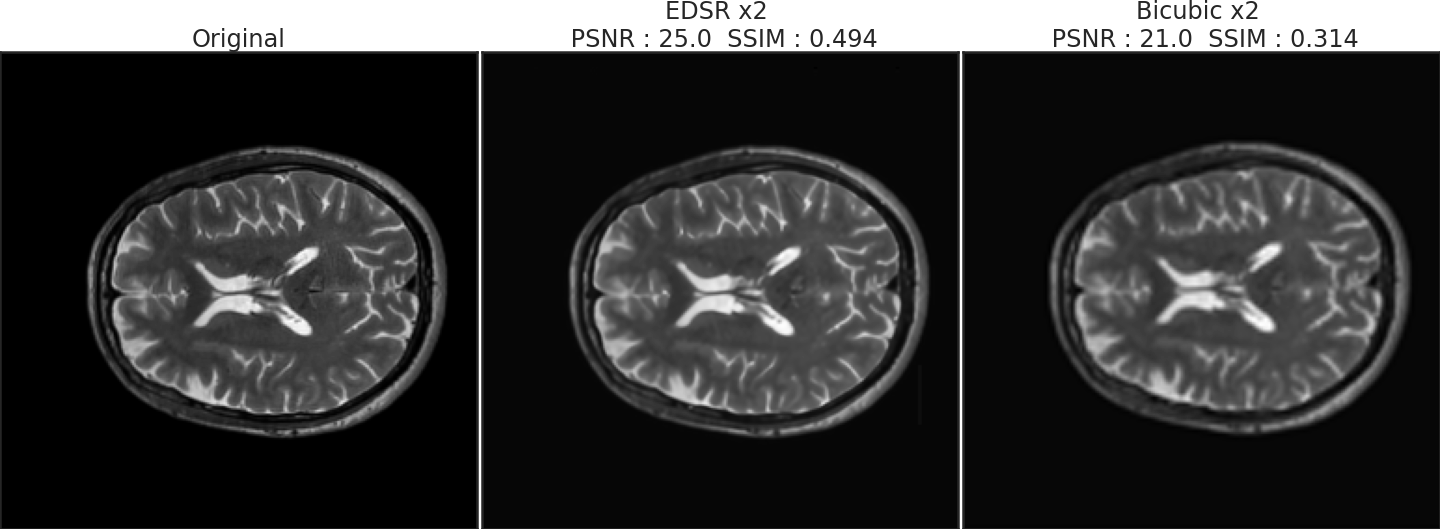
\includegraphics[scale=0.3]{./images/EDSR_comp_images_t2.png}
  \caption{\it (left) original image, (center) reconstruction performed with {\tt EDSR}, (right) reconstruction using the bicubic method for a T2-weighted image. The input in this case is not rotated.}
 \label{fig:edsr-upscale-t2}
\end{figure}

In this particular case, the {\tt EDSR} performed better that the bicubic algorithm, indeed the absolute difference image (in figure \ref{fig:edsr-diff-t2-b}) indicates much less high frequency component and a ``smoother'' visualization. 

For the {\tt WDSR} model, the three outputs are more consistents between each others and through the subjects they performs, on average, steadily better than the bicubic algorithm for T1-weighted NMR, as shown in figure \ref{fig:wdsr-score-slide-t1}:    

\begin{figure}[H]
  \centering
 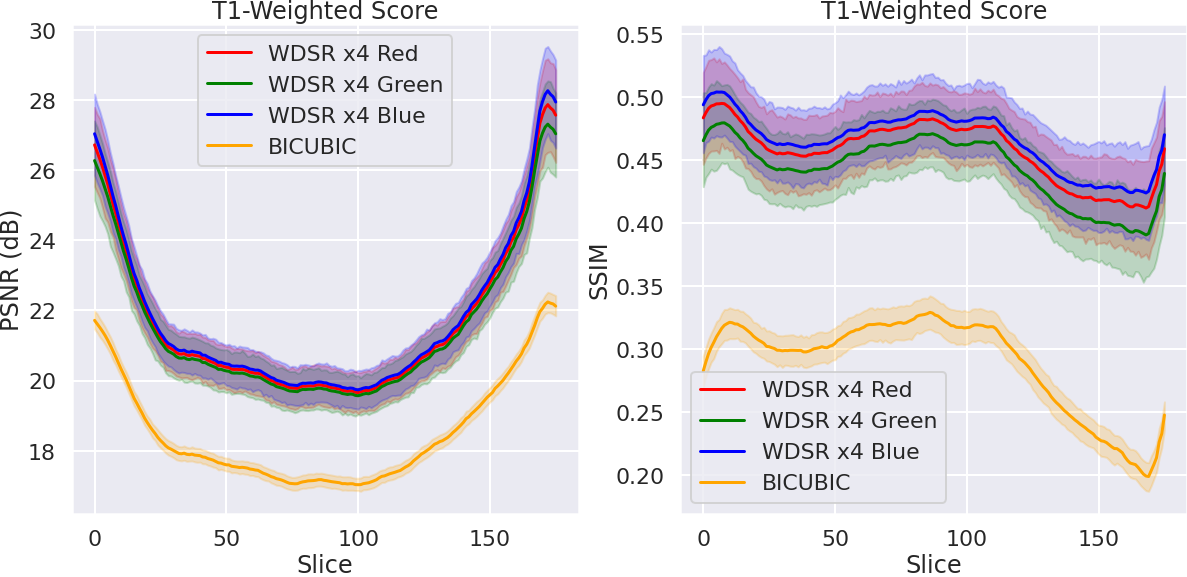
\includegraphics[scale=0.37]{./images/WDSR_score_slide_t1_all.png}
  \caption{\it Average trends of PSNR (left) and SSIM (right) for the three channels (Red, Blue, Green lines) of the Super Resolution WDSR model compared with the bicubic algorithm scores (Yellow) as functions of the slices. The average is performed for every patients and for every rotation, for T1-weighted NMRs.}
 \label{fig:wdsr-score-slide-t1}
\end{figure}

A recostruction performed starting from a donwscaled input $64 \times 64$ is shown in figure \ref{wdsr-upscale} for the two methods on a T1-weighted slice
\\
The result is clearly worse than the {\tt EDSR} cases since the $ \times 4$ down-scaling is quite heavy. 
Indeed, the recostruction shows a lot of artifacts, particularly on the scalp of the subjects and they are more evident for the slices upscaled with the {\tt WDSR}.
In both cases the upsampling methods introduce a bias on the background of the image which can spoil the quantitative result.
This effect can be explained if we consider that both models are not trained to upsample this kind of images, so the introduction of artifacts (such as background bias) may be a consequence of them trying to enhance the few signals gathered from the low-resolution inputs.

\begin{figure}[H]
 \centering 
  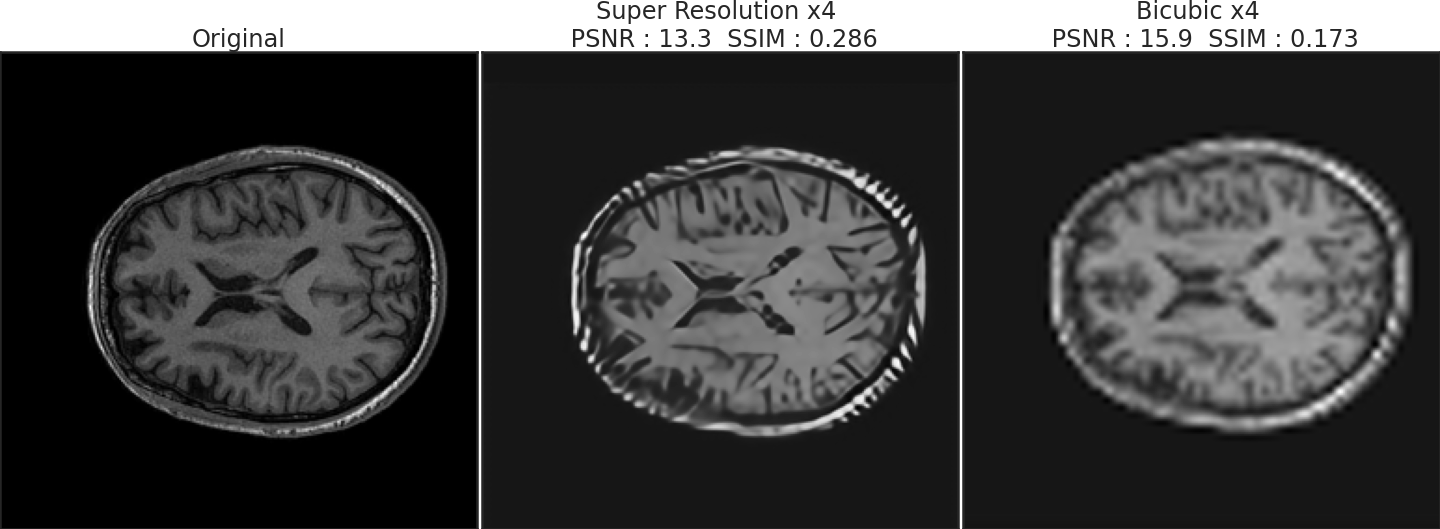
\includegraphics[scale=0.3]{./images/wdsr-comp-images.png}
  \caption{\it (left) original image, (center) reconstruction performed with {\tt WDSR}, (right) reconstruction using the bicubic method for a T1-weighted image. The input in this case is not rotated.}
 \label{wdsr-upscale}
\end{figure}

The results for T2-weighted images do not change if we compare the Bicubic upsample with the {\tt WDSR}, although it is possible to see that the scores are nearer to each others. 
The graphs are shown in figure \ref{fig:wdsr-score-slide-t2}.

\begin{figure}[H]
  \centering
 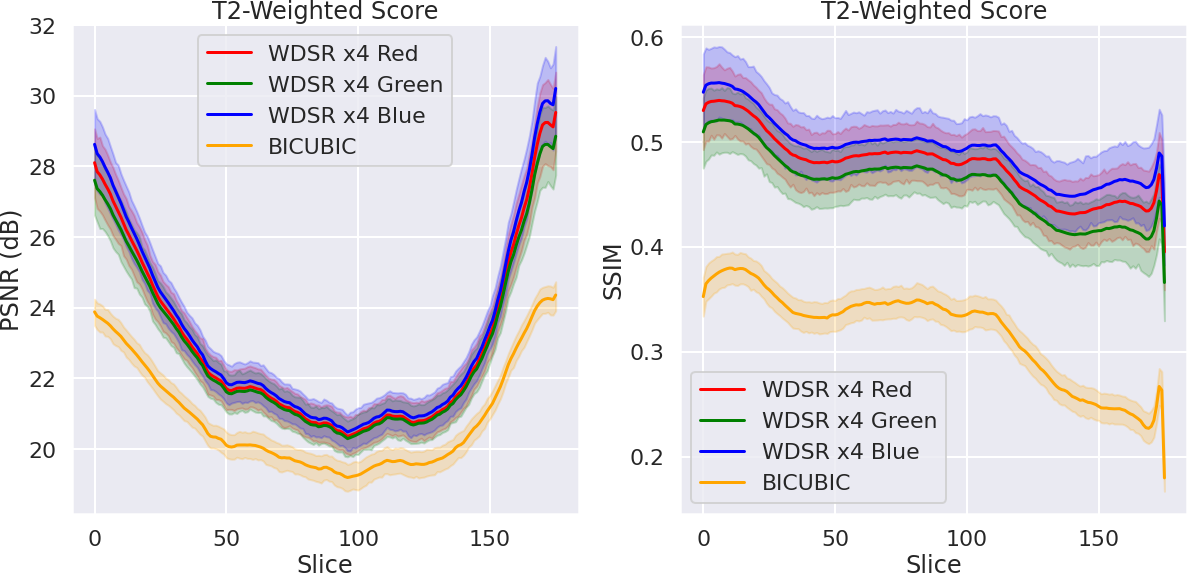
\includegraphics[scale=0.37]{./images/WDSR_score_slide_t2_all.png}
  \caption{\it Average trends of PSNR (left) and SSIM (right) for the three channels (Red, Blue, Green lines) of the Super Resolution WDSR model compared with the bicubic algorithm scores (Yellow) as functions of the slices. The average is performed for every patients and for every rotation, for T2-weighted NMRs.}
 \label{fig:wdsr-score-slide-t2}
\end{figure}

A recostruction performed starting from a donwscaled input $64 \times 64$  for a T2-weighted slice is shown in figure \ref{wdsr-upscale-t2} for the two methods:

\begin{figure}[H]
 \centering 
  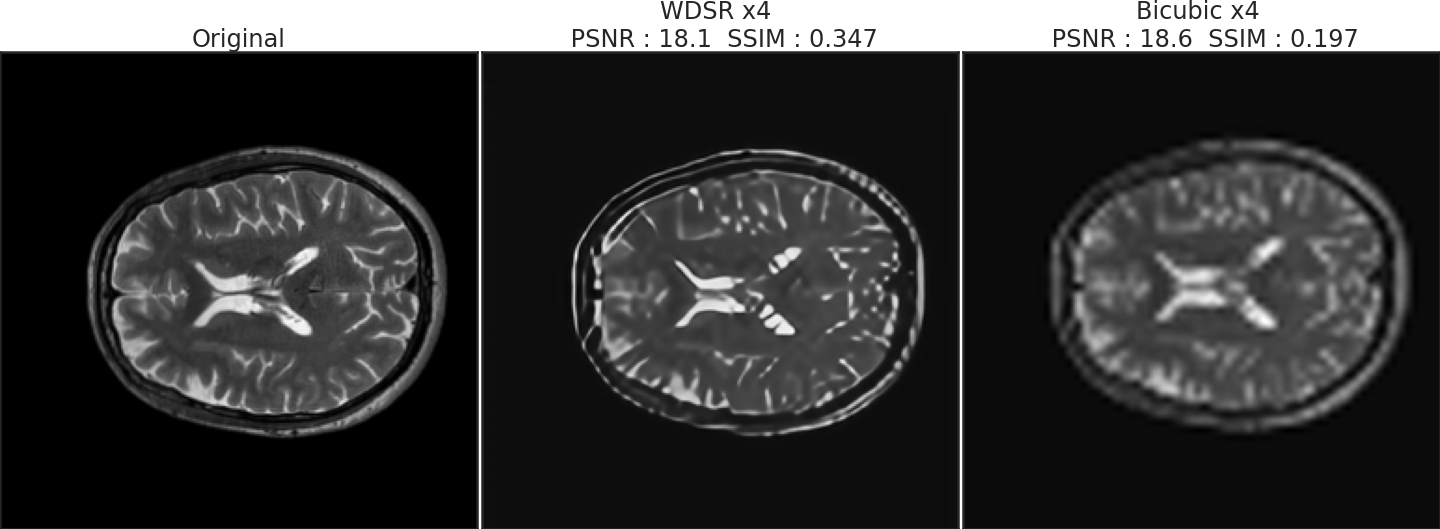
\includegraphics[scale=0.3]{./images/wdsr_comp_images_t2.png}
  \caption{\it (left) original image, (center) reconstruction performed with {\tt WDSR}, (right) reconstruction using the bicubic method for a T2-weighted image. The input in this case is not rotated.}
 \label{wdsr-upscale-t2}
\end{figure}

The {\tt WDSR} seems to obtain a smoother and less noisy than the bicubic up-sampling, both around edges and on 
Also, for T2-weighted images the number of artifacts in the scalp is reduced from figure \ref{wdsr-upscale}, which shows a T1-weighted reconstruction. 
Moreover, the background is much more dark than the T1 reconstruction. 

\section{Scores by Angle}

The next analysis focused on how the angle of rotation influences the final results. In figure \ref{fig:edsr-angles} it is possible to see again how the scores greatly varies between SR channels, with the green one beeing the best performer. The average trends (mediated between all patients and slides) exhibit the presence of privileged angles for every method tested.

\begin{figure}[H]
 \centering
 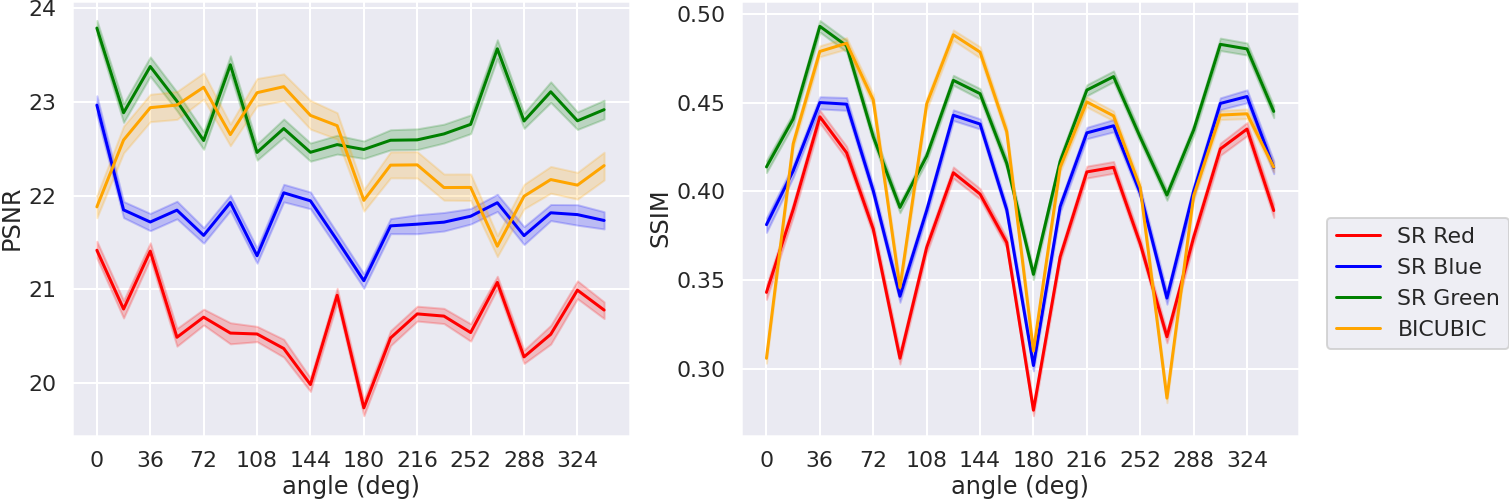
\includegraphics[scale=0.3]{./images/edsr-angles.png}
 \caption{\it average trends of PSNR (left) and SSIM (right) for {\tt EDSR} x2 and bicubic algorithm as functions of the input angle of rotations.}
 \label{fig:edsr-angles}
\end{figure}

The {\tt WDSR} shows a similar behaviour as the SSIM score in the previous case where angles different from $n \frac{\pi}{2}$ with $n = 0, 1, 2, 3$ performs better, as shown in figure \ref{fig:wdsr-angles}.   

\begin{figure}[H]
 \centering
 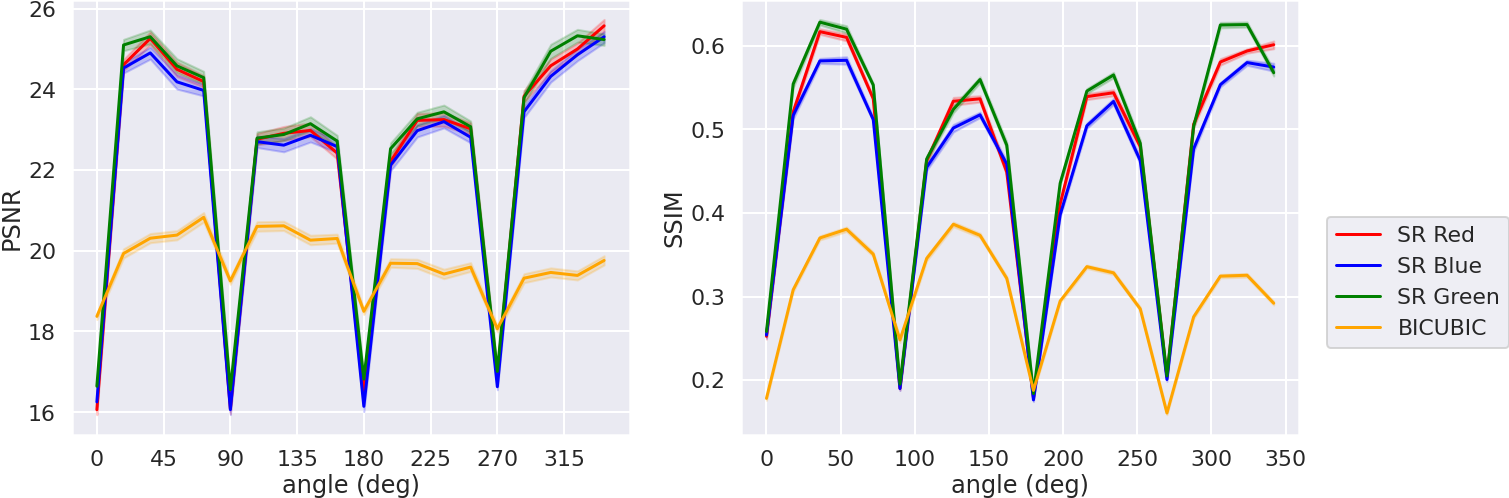
\includegraphics[scale=0.3]{./images/wdsr-angles.png}
 \caption{\it average trends of PSNR (left) and SSIM (right) for {\tt WDSR} x4 and bicubic algorithm as functions of the input angle of rotations.}
 \label{fig:wdsr-angles}
\end{figure}

The results are congruos with what has been shown in the previous section in which the three channels (Red, Green and Blue lines) are consistent between themselves.
In both cases there are angles for which the bicubic algorithm performs better than SR.

If we take a look at the images upscaled by x2 methods in figure \ref{fig:edsr-angle-18}, the difference between input angles is not really noticeable: 

\begin{figure}[H]
 \centering
 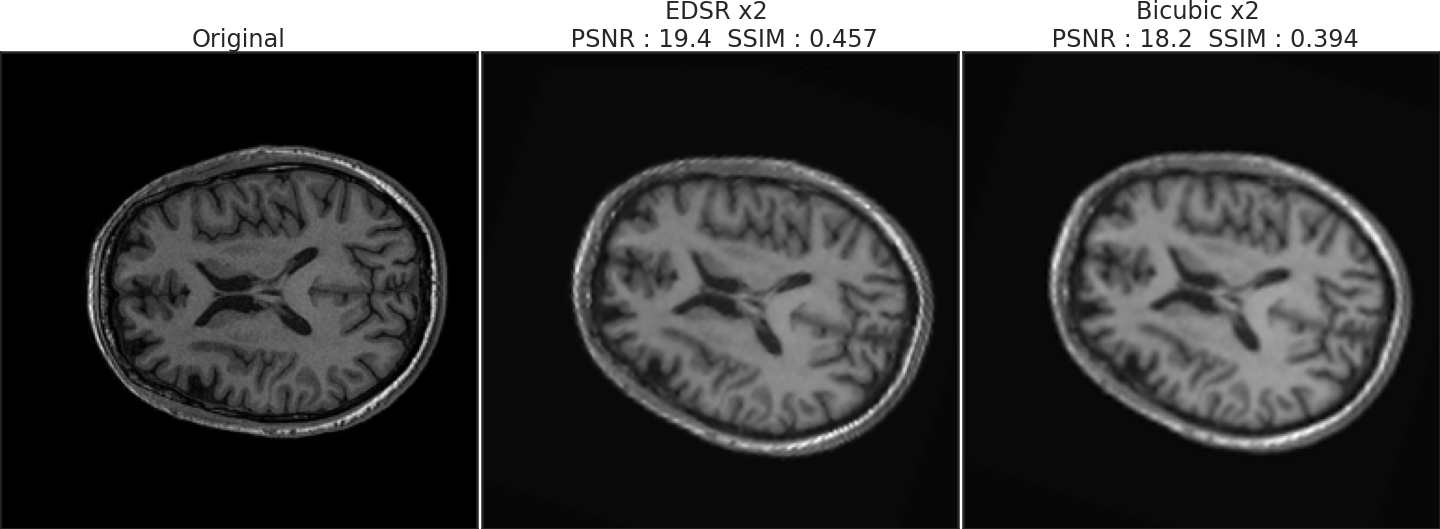
\includegraphics[scale=0.3]{./images/edsr_angle_18.png}
 \caption{\it comparison between {\tt EDSR} x2 and bicubic, if compared with the images above, the level of recostruction is really similar to slices without rotations in figure \ref{fig:edsr-upscale}}
 \label{fig:edsr-angle-18}
\end{figure}

On the other hand, the {\tt WDSR} x4 upscaling shows far less artifact on angles different from $n\frac{\pi}{2}$ as can be seen in figure \ref{fig:wdsr-angle-18}:

\begin{figure}[H]
 \centering
 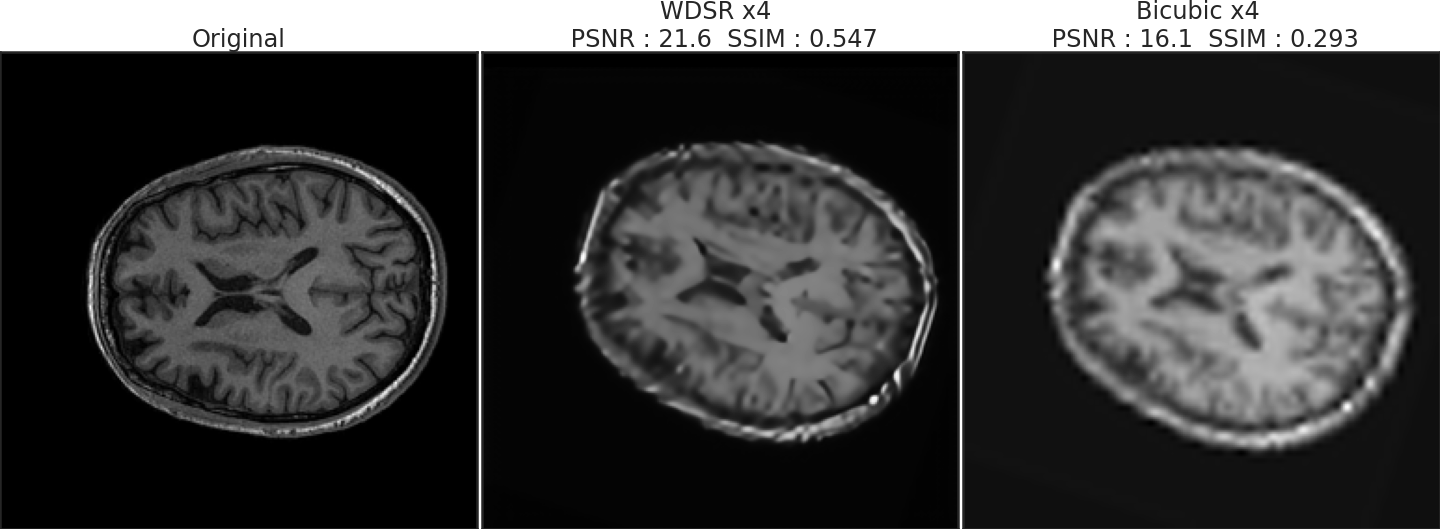
\includegraphics[scale=0.3]{./images/wdsr_angle_18.png}
 \caption{\it comparison between {\tt WDSR} x4 and bicubic, if compared with the images above, the level of recostruction is better than slices without rotations in figure \ref{wdsr-upscale}. Indeed the number of artifacts seems to be far lower than before for {\tt WDSR}.}
 \label{fig:wdsr-angle-18}
\end{figure}

This can be due to different reasons: firstly, by rotating the images we technically performs an interpolation, particularly for angles differents from multiple of 90°; this can enhance or deteriorate lines and textures of the images and by results, strengthen or weaken the reconstruction of the methods. 
Secondly, the DIV2K dataset in which the models are trained and tested is intrinsically oriented: this means that if the images are not rotated during training, the models could have learnt a privileged angle of orientation for shapes and texture.
Interestingly, as stated in \cite{wdsr} for {\tt WDSR} and in \cite{edsr} for {\tt EDSR}, both models should have been trained by augmenting the dataset with randoms flips and rotations of the input images. 
Another possibility is the convolutional layers, which compose the majority of deep learning models, are not invariant for rotations, but only for transitions, that may introduces variations in the results.

\newpage

\section{Error localization}

The following section will focus on where the error is localized in the images and how it is distributed. 
For doing that I computed the pixel-wise absolute difference between the original slice and the correspondent super-resolved one. As can be seen in figure \ref{fig:abs_diff_x2} the major differences lie in the scalp of the subjects, which tends to be the most uninteresting part.

\begin{figure}[H]
 \centering
 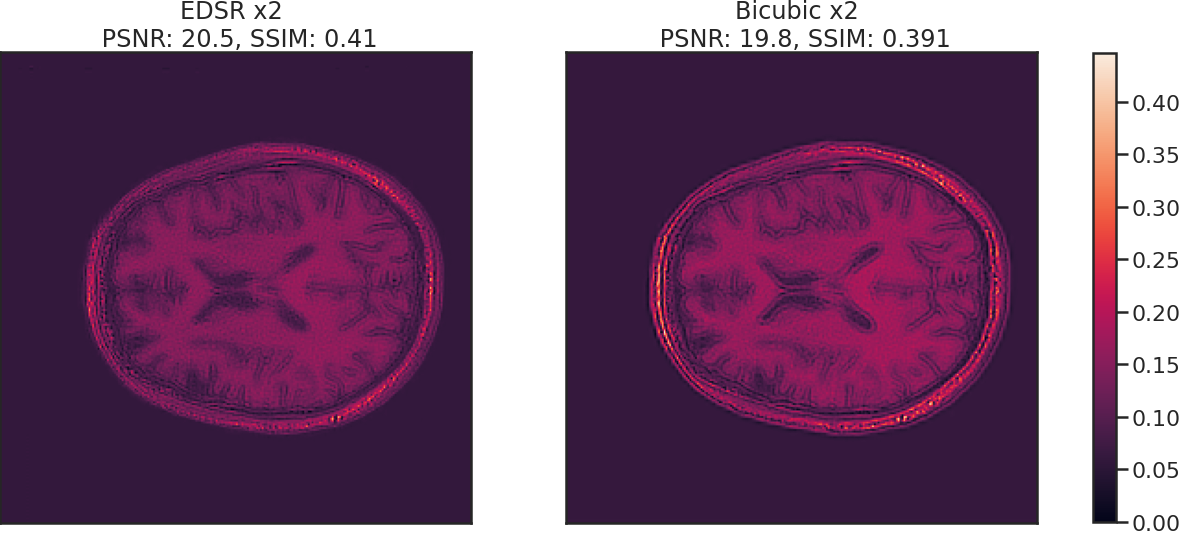
\includegraphics[scale=0.4]{./images/diff-edsr.png}
 \caption{\it Absolute differences for {\tt EDSR} reconstruction (left) and bicubic (right), for a T1-weighted image. In both cases, the major differences seems to lies in the scalps of the subjecs. Though, it can be seen that the background is not zero, which means it has an impact on the scores.}
 \label{fig:abs_diff_x2}
\end{figure}

It is also clear by the differences, that the bias introduced by the two methods influences the results since there is a non-zero background which makes up a large part of the images. Indeed, by looking at the error distribution in figure \ref{fig:histo-edsr}, it appears that the background component is the most relevant part. 
However, by being prevalent on both methods, it does not influence the relative results.
The second, and lower, peak of the two distributions represents the {\it brain component} of the images: by looking at them we can see that the distribution relative to the SR model is narrower and slightly shifted towards lower intensities, therefore justifying the better scores achieved by the model.
Both histograms are mostly composed by values lower than 0: this means that the two models over-estimate most of the pixel values.

\begin{figure}[H]
 \centering
 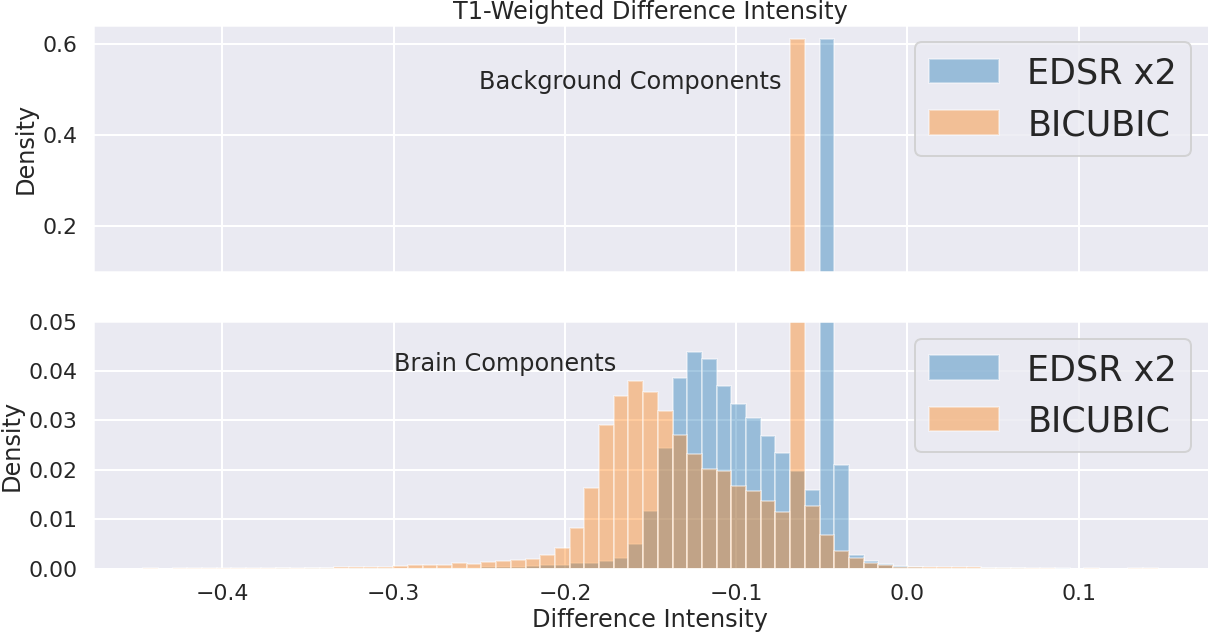
\includegraphics[scale=.35]{./images/EDSR_diff_histo_t1.png}
 \caption{\it Histograms of the distribution of differences pixel-by-pixel for the reconstruction performed by EDSR (Blue) and by the bicubic algorithm (Orange), for a T1-weighted NMR. The histogram has been cut between 0.05 and 0.1 on the $y$ axis to better represent the lower parts.}
 \label{fig:histo-edsr}
\end{figure}

In the case of a T2-weighted sample, I show in figure \ref{fig:edsr-diff-t2-b} that the behaviour seems to be inversed: indeed this time the high frequency components of the differences are focused on the inner parts of the image and in particular around edges.

\begin{figure}[H]
 \centering
 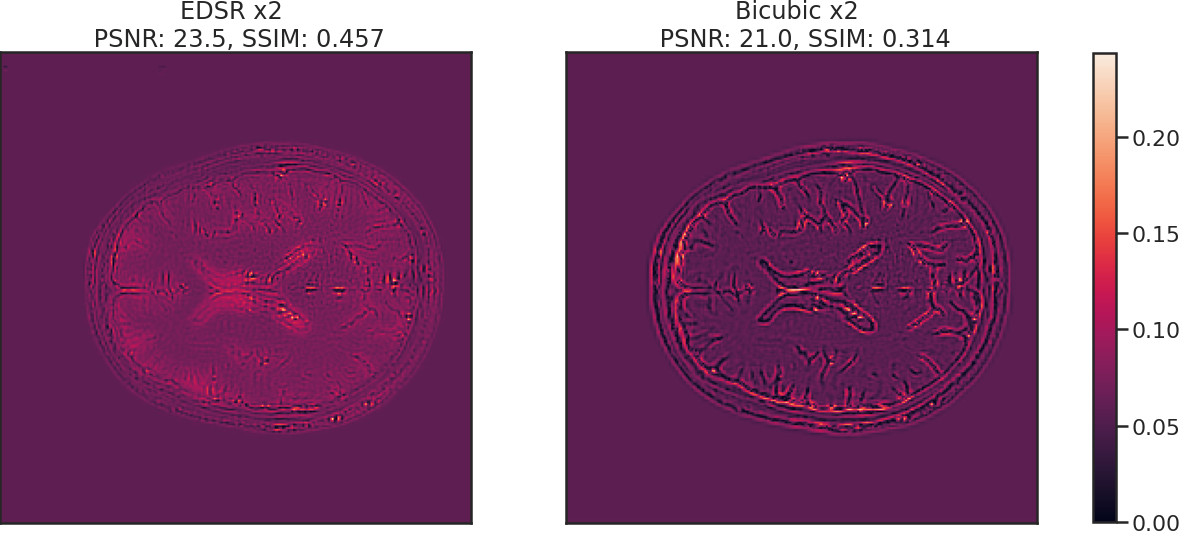
\includegraphics[scale=0.4]{./images/EDSR_diff_t2.png}
 \caption{\it Absolute differences of Super resolved image obtained with {\tt EDSR} (left) and bicubic (right) for T2-weighted NMR. This time the major differences seem to be mostly located on the inner parts of the sample, in particular around edges.}
 \label{fig:edsr-diff-t2-b}
\end{figure}

Also, the distribution of those differences is more concentrated around the peak of density, which, again, represents the background components, that is not zero. 
This concentration (and simmetry, in case of the bicubic upsample) is due to fact that there are much less white and gray pixels and a majority of dark-ish ones.

\begin{figure}[H]
 \centering
 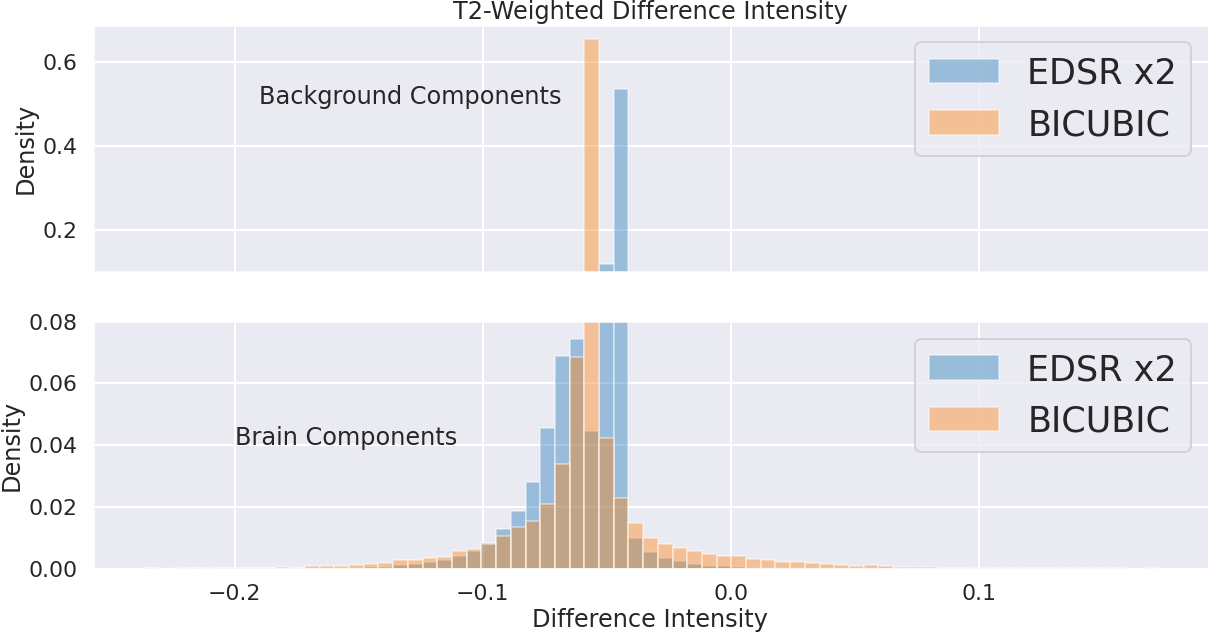
\includegraphics[scale=0.3]{./images/EDSR_diff_histo_t2.png}
 \caption{\it Histograms of the distribution of differences pixel-by-pixel for a reconstruction performed by EDSR (Blue) and by the bicubic algorithm (Orange), for a T2-weighted NMR. The histogram has been cut between 0.08 and 0.1 on the $y$ axis to better represent the lower parts.}
 \label{fig;edsr-diff-histo-t2}
\end{figure}

The same comparisons can be made also for {\tt WDSR} and in general for an up-sampling scale factor of $\times 4$. In figure \ref{fig:wdsr-diff-t1} I show the absolute differences of a T1 sample upscaled from $64 \times 64$ to HR.  

\begin{figure}[H]
 \centering
 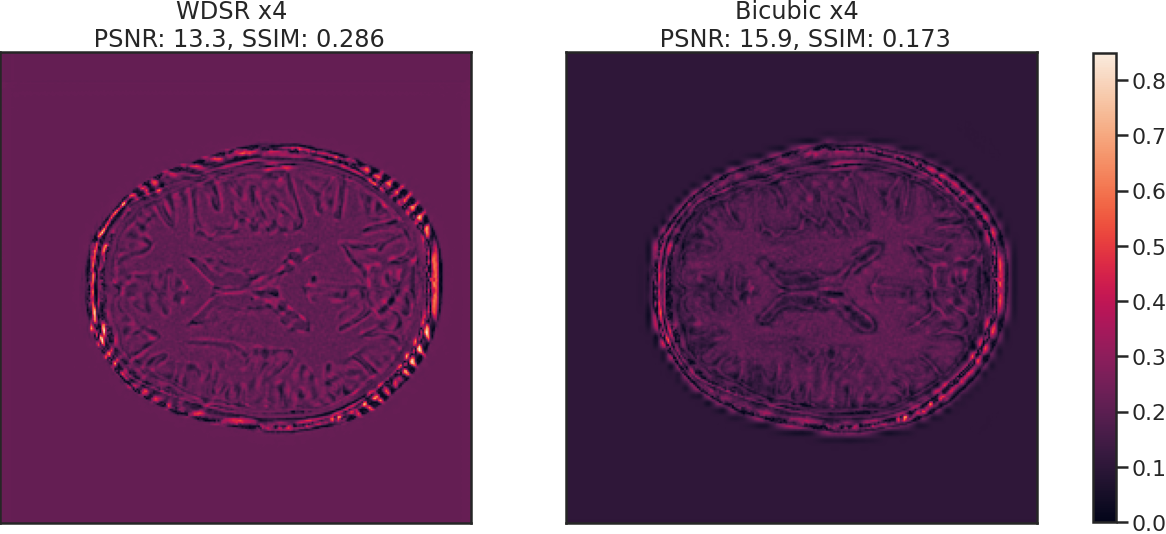
\includegraphics[scale=0.4]{./images/WDSR_diff_t1.png}
 \caption{\it Absolute differences of Super resolved images obtained with {\tt WDSR} (left) and bicubic (right) for a T1-weighted NMR. Also in this case the major differences seems to be focused on the scalp of the subjects.}
 \label{fig:wdsr-diff-t1}
\end{figure}

First of all, also in this case the major differences are located around the scalp, this visualization also highlights better the artifacts created during the upsampling for both reconstractions.
Another problem, is the strong background components of the {\tt WDSR}. upsampling, which is much more evident than in the bicubic case. 
In the histograms in figure \ref{fig:wdsr-diff-histo-t1} is shown the distributions of the differences of the two reconstructions:

\begin{figure}[H]
 \centering
 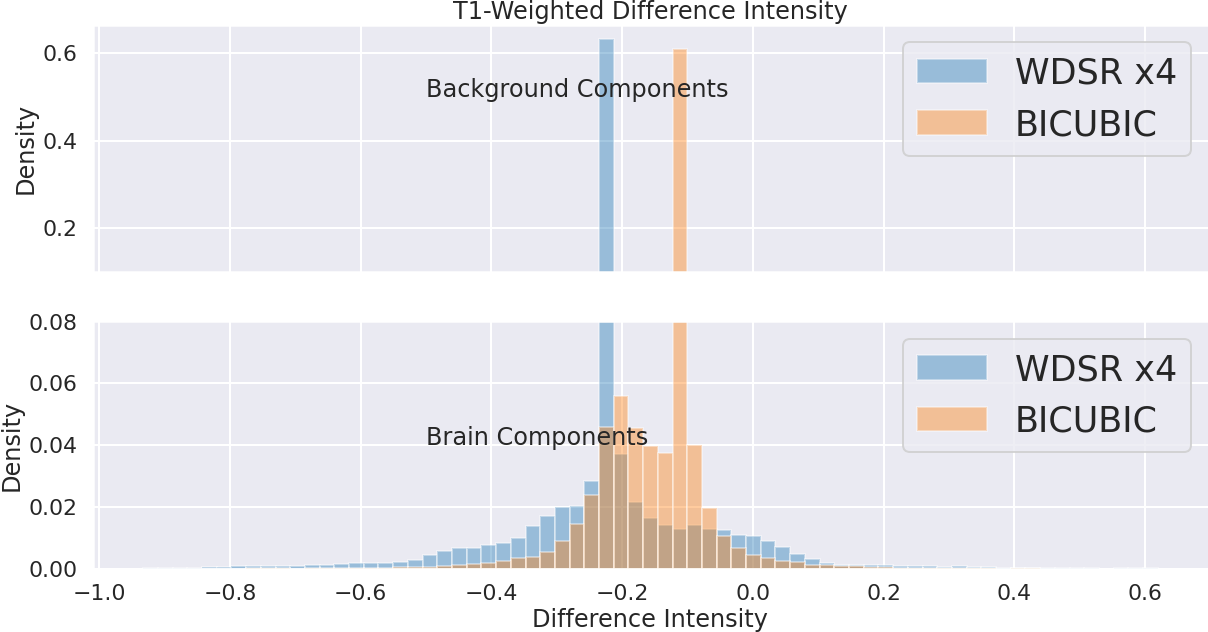
\includegraphics[scale=0.3]{./images/WDSR_diff_histo_t1.png}
 \caption{\it Histograms of the distribution of differences pixel-by-pixel for a reconstruction performed by EDSR (Blue) and by the bicubic algorithm (Orange), for a T2-weighted NMR. The histogram has been cut between 0.08 and 0.1 on the $y$ axis to better represent the lower parts.}
 \label{fig:wdsr-diff-histo-t1}
\end{figure}

The same considerations that have been expressed for the previous cases, can be made also in this one: by looking at the distributions, both models over-estimate the majority of pixels in the images. 

In figure \ref{fig:wdsr-diff-t2} is shown the absolute difference between the original images and the two $\times 4$ reconstructions performed respectively by {\tt WDSR} and the bicubic.

\begin{figure}[H]
 \centering
 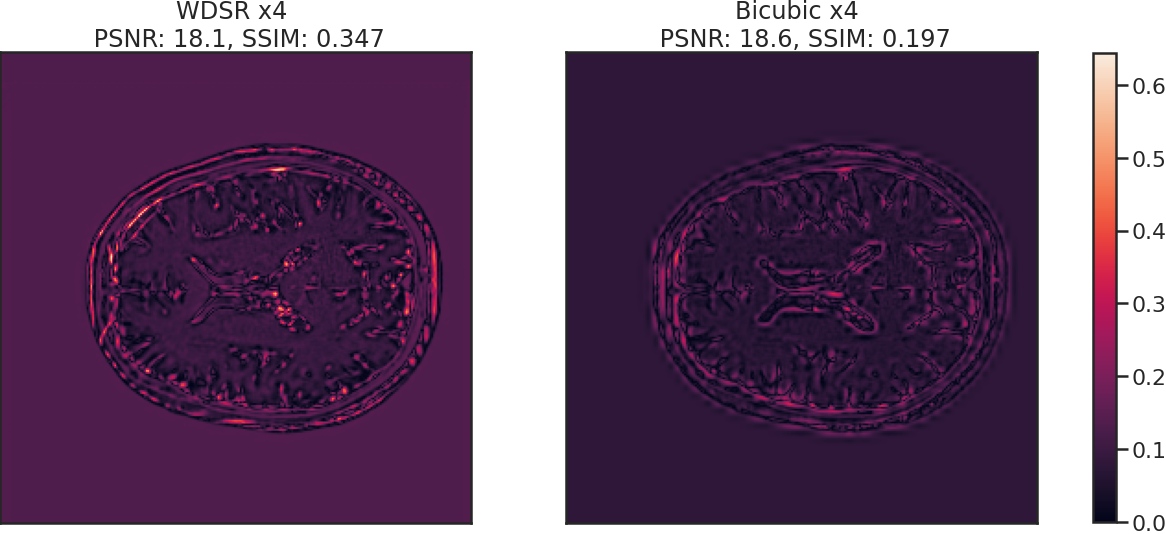
\includegraphics[scale=0.4]{./images/WDSR_diff_t2.png}
 \caption{\it Absolute differences of Super resolved images obtained with {\tt WDSR} (left) and bicubic (right) for a T2-weighted NMR.}
 \label{fig:wdsr-diff-t2}
\end{figure}

In figure \ref{fig:wdsr-diff-histo-t2} is shown the relative histograms of distributions of differences for the slice shown above.

\begin{figure}[H]
 \centering
 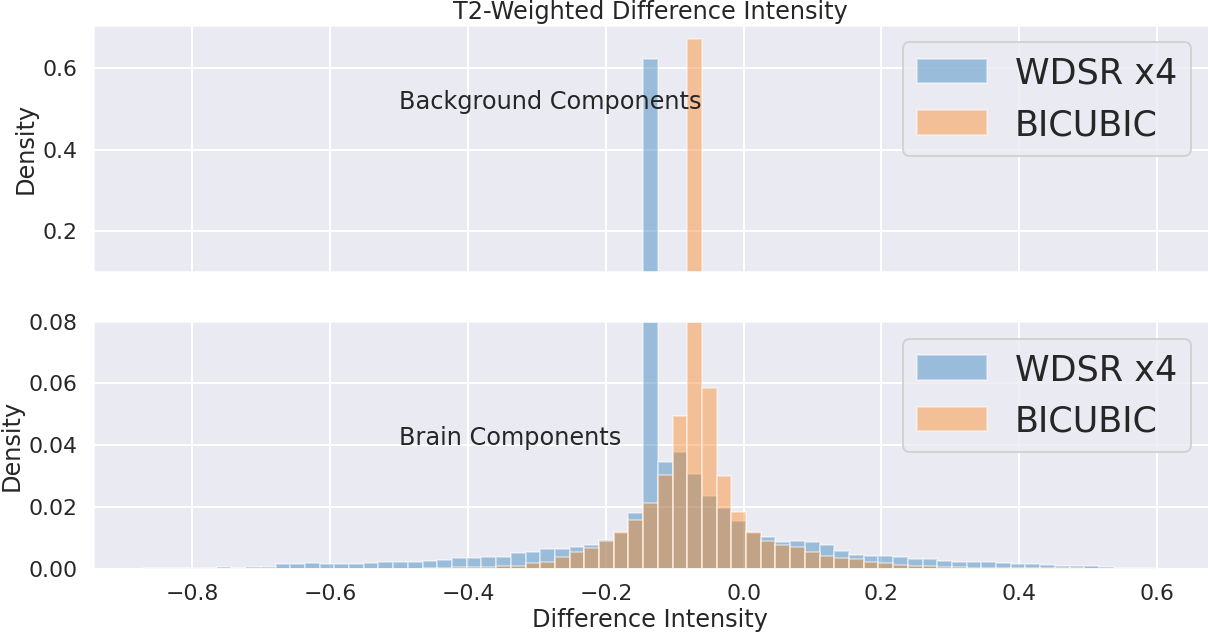
\includegraphics[scale=0.3]{./images/WDSR_diff_histo_t2.png}
 \caption{\it Histograms of the distribution of differences pixel-by-pixel for a reconstruction performed by EDSR (Blue) and by the bicubic algorithm (Orange), for a T2-weighted NMR. The histogram has been cut between 0.08 and 0.1 on the $y$ axis to better represent the lower parts.}
 \label{fig:wdsr-diff-histo-t2}
\end{figure}

In this case the distribution seems to be more spreaded and almost symmetric around the peak, again sligtly shifted towards negatives values, which indicates an over-estimation of pixel gray scale values for the two reconstructions. 

The next analysis will focus on the study of how reconstructions performs with a standard post-processing tool for NMR and on the analysis of the same data by removing the background. 

\section{Brain Extraction}

To avoid background related problems, I extended the analysis to images where the background and the scalp were removed with FSL BET (Brain Extraction Tool)\cite{fsl}.
FSL is a standard post-processing tool for NMR, it works by creating a binary mask for every slice and then applies it to the images: in this way is possible to extract only the relevant information from data. 
A binary mask is a tensor of zeros and ones with the same dimension as the original NMR, the ``ones'' correspond with the pixel we want to preserve. 
An example is shown in figure \ref{fig:mask-ex}:

\begin{figure}[H]
  \centering
  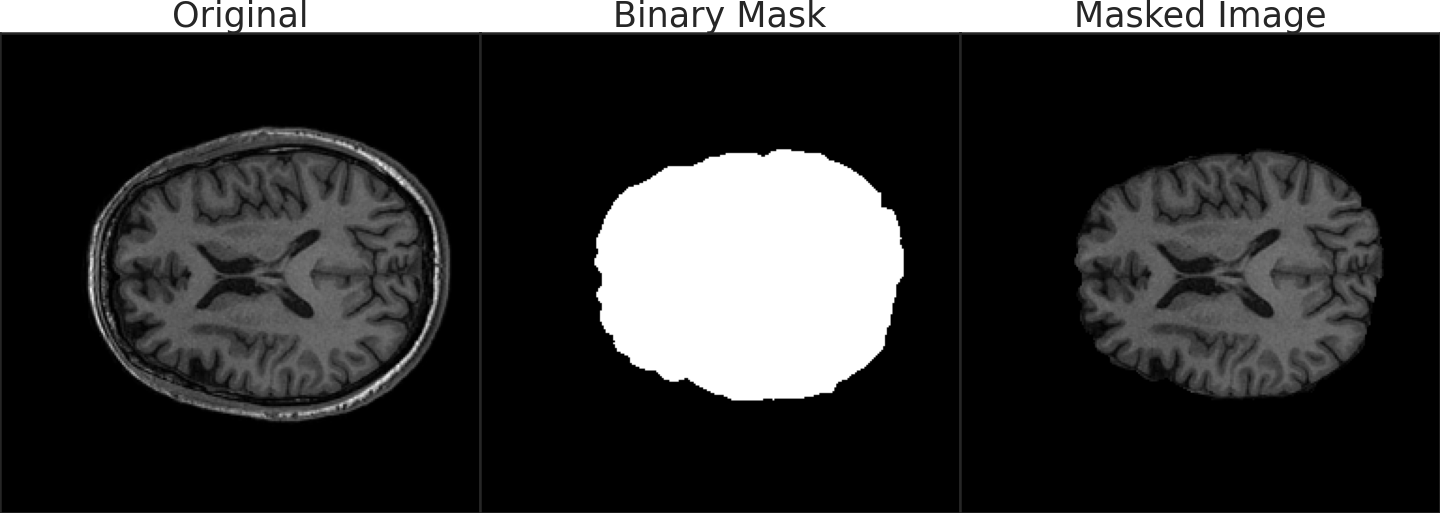
\includegraphics[scale=0.28]{./images/mask_example.png}
  \caption{\it Example of application of a mask on one of the slices of the original 3D map. (left) Original image, (center) Mask obtained from FSL BET and (right) Mask applyed to the original image. }
  \label{fig:mask-ex}
\end{figure}

I reported two different approaches for a single patient: firstly, three different binary masks for original images, Super Resolved reconstructions and bicubic ones were extracted. In this way it is possible to quantify how well a standard post processing tool like BET performs on images obtained by upsampling. 
Secondly, I masked all three reconstruction with the same binary mask, obtained from the original high resolution NMR, in this way it is possible to compare directly the reconstruction capabilities of the methods, without including uninteresting data.
The first analysis how well BET works on the reconstructed images, therefore I will consider distinct masks applied separately to the results.
As shown in figure \ref{fig:bet-example}, Brain Extraction Tool not only removes the background, but also the entire scalp, which was shown to contains the main differences from the original image.

\begin{figure}[H]
  \centering
  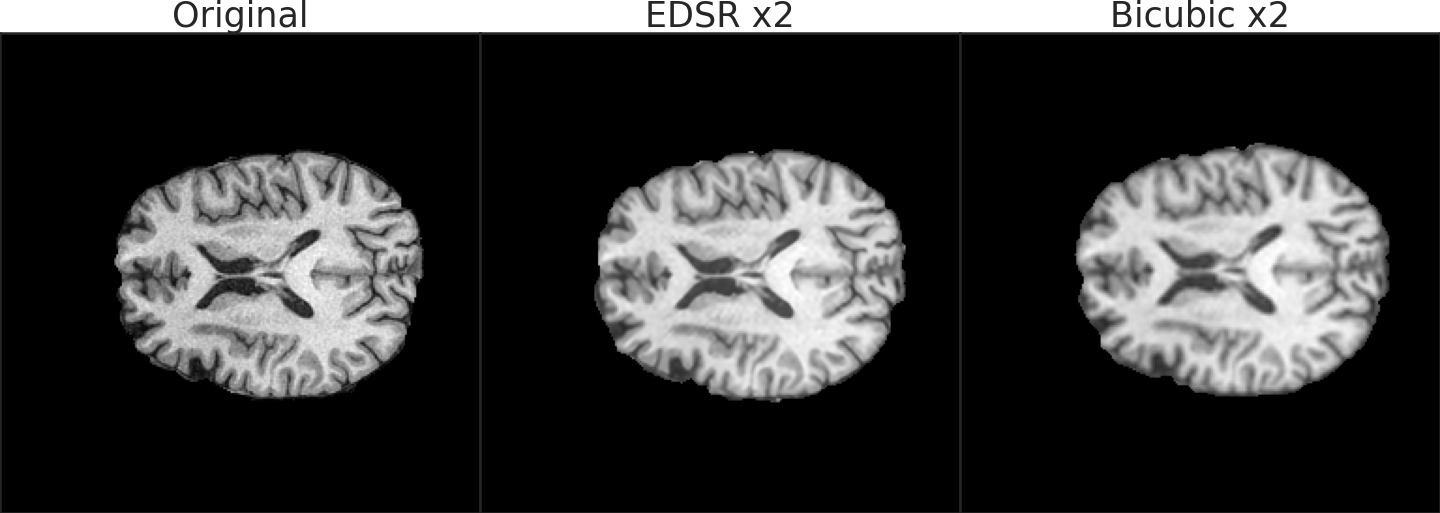
\includegraphics[scale=0.28]{./images/bet_example.png}
 \caption{\it Examples of Brain Extraction for original image (left), EDSR image (center) and Bicubic results (right). The binary masks are different for the three images.}
 \label{fig:bet-example}
\end{figure}

% Indeed, by comparing the scores on every slice pre and post BET, the performance improvement is clear. 
% For {\tt EDSR} the results are reported in figure \ref{fig:pre-post-bet}: in the upper graphs are shown the trends for PSNR and SSIM of 1 patient weighted $T_1$ for no rotation while on the graphs below the trends for the same NMR after the BET. 
% It is possible to see how the scores greatly improve in the second case, showing that the background/scalp removal has a significant impact on performances and at the same time, the Super Resolution's scores are still better than the bicubic's.
% As a side note, the initial and final slices are cut from the analysis of PSNR since they are completely black pictures and the scores diverge, while the SSIM reaches one.
% 
% \begin{figure}[H]
%   \centering
%   \includegraphics[scale=0.27]{./images/pre_bet_edsr.png}
%   \includegraphics[scale=0.27]{./images/betted_x2_slide.png}
%  \caption{\it comparisons between trends for one patients of PSNR (left) and SSIM (right) of results obtained from {\tt EDSR} and bicubic algorithm. The upper graphs refers to images pre Brain Extraction while the lower ones post Brain Extraction. After the removal of background and scalp, the scores improve for both methods, while still showing better performances for Super Resolution}
%  \label{fig:pre-post-bet}
% \end{figure}
% 
% For the {\tt WDSR} model the results after the brain extraction are really close to the ones shown for the {\tt EDSR} and are reported with same structure in figure \ref{fig:pre-post-bet-2}:
% 
% \begin{figure}[H]
%   \centering
%   \includegraphics[scale=0.3]{./images/pre_bet_wdsr.png}
%   \includegraphics[scale=0.3]{./images/betted_x4_slide.png}
%  \caption{\it Comparisons between trends for one patients of PSNR (left) and SSIM (right) of results obtained from {\tt WDSR} and bicubic algorithm. The upper graphs refers to images pre Brain Extraction while the lower ones post Brain Extraction. After the removal of background and scalp, the scores improve for both methods, while showing better performances for Super Resolution.}
%  \label{fig:pre-post-bet-2}
% \end{figure}
% 
% Again, both methods shows a huge score improvement with the {\tt WDSR} being the best performer overall.

In figures \ref{fig:edsr-bet-diff} and \ref{fig:wdsr-bet-diff} the differences pixel by pixel between super resolution's results and the original image are reported side-by-side with the corresponding Bicubic results.

\begin{figure}[H]
\centering
 \includegraphics[scale=0.4]{./images/edsr_diff_betted}
 \caption{\it Absolute differences for Super Resolution (EDSR, left) and bicubic (right). The images are obtained by computing a pixel-wise absolute difference with the original slice. We can see the main dissimilarities on the border of the two images, meaning that the BET didn't catch all the relevant informations on the reconstructed images.}
 \label{fig:edsr-bet-diff}
\end{figure}

\begin{figure}[H]
\centering
 \includegraphics[scale=0.4]{./images/wdsr_diff_betted}
 \caption{\it Absolute differences for Super Resolution {\tt WDSR}, left) and bicubic (right). In this case, the principal dissimilarities are not focused only on the outer parts of the brain and that is understandable, given the high level of downsampling.}
 \label{fig:wdsr-bet-diff}
\end{figure}

In the first case (figure \ref{fig:edsr-bet-diff}) we can see the main dissimilarities are on the border of the two brains, meaning that BET did not catch all the relevant informations on the reconstructed sample or, otherwise, the up-sampling highlighted . 
In any case, there some differences between masks, which can be quantified with an {\it Intersection over Union} (IoU), as described below.  

In the second case (figure \ref{fig:wdsr-bet-diff}), the principal dissimilarities are not focused only on the outer parts of the brain, accordingly to what have been shown before, and that is understandable, given the high level of downsampling. 
Again there some discrepancies between images aroun the border, meaning that during re-upsample some of the informations are lost or over-amplified with respect to the original image.  

The histogram of the distribution of differences in figure \ref{fig:histo-bet-edsr} shows how the background component is now shifted towards 0, implying that is not considered in the score computations. 
The distributions also shows a spread and a shift towards higher differences of the brain component: this is probably due to the higher contrast in the images obtained by brain extraction.

\begin{figure}[H]
 \centering
 \includegraphics[scale=0.4]{./images/histo_bet_edsr.png}
 \caption{\it Histogram of differences for an image obtained with x2 up-sampling and after Brain Extraction. The background componenent is completely shifted towards zero, while the Brain componentent spreaded and shifted toward higher intensity for contrast manipulation. The distributions for the two methods are nearly identical. The histogram has been cut on the y axis between 0.07 and 0.2 to better represent the Brain Component}
 \label{fig:histo-bet-edsr}
\end{figure}

As a last evaluation I considered the Intersection over Union (IoU) score, which quantifies the overlap between different masks. 
The IoU is defined as: 

\begin{equation}
 IoU = \frac{A \cap B}{A \cup B}
\end{equation}

where $A$, in this case, is the binary mask obtained by the original slice, while $B$ is the mask obtained by one of the upsampling methods.
The trends of IoU for the two models compared with the bicubic algorithm can be found in figure \ref{fig:iou}

\begin{figure}[H]
 \centering
 \includegraphics[scale=0.35]{./images/iou_scores.png}
 \caption{\it Trends of IoU scores for the different upsamplig methods. (left) comparison between the mask obtained from {\tt EDSR} and bicubic recostructions and (right) same graph for {\tt WDSR} and bicubic. 
 Notice that some slices are cut from comparisons since they are black images and both intersection and union are 0.}
 \label{fig:iou}
\end{figure}

The comparisons between IoU in the {\tt EDSR} do not shows much of a difference with the bicubic algorithm. On the other hand, {\tt WDSR} seems to be slightly penalized: that is most likely due to the artifacts present in the scalp of the subjects shown
in figure \ref{wdsr-upscale} interfering with the brain extraction, which may makes the super-resolution model with this level of down-sampling less adapt to work with BET-like softwares
\\
The second analysis proposed in this section regards how the upsampling methods performs considering the same mask applied for all the reconstruction: so that I can compute the scores considering only the same portion of the images, without worriying about background effects. 
Since the original High Resolution NMR is supposed to represents an objective ``truth'' for our study, the best available mask is of course the one acquired from its brain extraction.
For {\tt EDSR}, the results in figure \ref{fig:edsr-bet-same-mask} shows the average trends of PSNR and SSIM pre and post brain extraction for the selected patient, mediated over the rotations angle.

\begin{figure}[H]
 \centering
 \includegraphics[scale=0.35]{./images/EDSR_score_t1_prebet.png} 
 \includegraphics[scale=0.35]{./images/EDSR_score_slide_t1_betted.png}
 \caption{\it Average trends of PSNR (left) and SSIM (right) for the three channels (Red, Blue, Green lines) of the Super Resolution {\tt EDSR} model compared with the bicubic algorithm scores (Yellow) as functions of the slices. Above are the results pre brain extraction while below the ones post brain extraction. The average is performed for one patient and for every rotation, for T1-weighted NMRs.}
 \label{fig:edsr-bet-same-mask}
\end{figure}

By comparing the pre and post BET performances, it is clear that the differences between channels become much lower, which may means that the discrepancies measured in the pre BET trends comes from artifacts and backgrounds related to ``false-features'' extrapolation which are different between channels and mitigated (or entirely removed) when masking the slices.
However, at same time, the score discrepancies between bicubic and SR also become much lower than pre-BET, meaning that, on average, the background components does favour the Super-Resolution, but still {\tt EDSR} beats the upsampling of the bicubic by a fair amount after brain extraction.
\\
The same comparisons for {\tt WDSR} in figure \ref{fig:wdsr-bet-same-mask} shows very similar results:

\begin{figure}[H]
 \centering
 \includegraphics[scale=0.32]{./images/WDSR_score_t1_prebet.png}
 \includegraphics[scale=0.32]{./images/WDSR_score_slide_t1_betted.png}
 \caption{\it  Average trends of PSNR (left) and SSIM (right) for the three channels (Red, Blue, Green lines) of the Super Resolution {\tt WDSR} model compared with the bicubic algorithm scores (Yellow) as functions of the slices. Above are the results pre brain extraction while below the ones post brain extraction. The average is performed for one patient and for every rotation, for T1-weighted NMRs.}
 \label{fig:wdsr-bet-same-mask}
\end{figure}

Indeed, even in this case, the SR performs better than the bicubic algorithm for all three channels, which are very consistent with each others. This may indicates that the differences between channels derived by what each of them extrapolate from the background, in terms of bias and artifacts.

\chapter{Conclusions}
In this work I developed two novel frameworks for Deep Learning called {\tt Byron} in C++ and {\tt NumPyNet} in Python, the former focused on CPU optimizatioon while the latter focused on readability.
I tested the computational performances of {\tt Byron} for the most important layers in image analysis against the python library {\tt Tensorflow}.   
\\
Moreover, the work extended to implementing and testing two models for super-resolution, {\tt EDSR} and {\tt WDSR}, on NMR images, which represent a new benchmark for those deep networks, originally trained and tested only on {\tt DIV2K}.
On average, the models show better reconstruction capabilities on the most interesting parts of the brain compared with the bicubic algorithm, although they introduce artifacts and biases: this may be a consequence of them trying to enhance the few signals gathered from low-resolution input and ``seeing'' false-features inside the background of the slices.
Testing {\tt EDSR}, an RGB model, on a gray-scale dataset also highlighted great variability between the three output channels, while {\tt WDSR} seems to be more stable in this respect.
On the other hand though, while {\tt EDSR} results do not exhibit visible differences across angle of rotations, {\tt WDSR}'s ones has been shown to improve for rotations different from multiples of 90°, possibly showing that its action is not invariant with rotations.
The localization of errors through a pixel-wise absolute difference between reconstructions and high-resolution NMRs indicates that for both algorithms the major discrepancies are localized around the scalps of the subjects, which tends to be the most uninteresting section of the brains. 
Although, they also highlight that the background components of the images are 
Thus, the brain extraction has been helpful in removing both background effects and the high level of discrepancy in the scalp. 
This, in turn, lowered the differencies of performances between super-resolution RGB channels and bicubic algorithm for both models {\tt EDSR} and {\tt WDSR}, while also showing that the SR still shows promising results in terms of reconstruction  of biomedical iamge, which is an indication of how well this models can generalize the ``knowledge'' acquired during training on a completely different dataset such as DIV2K, which does not contain any data about NMRs or other kind of biomedical image.
\\
Some future developments for the work may include:

\begin{itemize}
 \item An exhaustive algorithm for training in {\tt Byron} to investigate the concept of {\it transfer learning}: namely,  storing knowledge gained while solving a problem and re-applying it to a different, but related, task. In this case, we can use the same dataset of NMR to continue the training of {\tt EDSR} and {\tt WDSR} starting from the parameters obtained by the respective authors. 
 Of course, the networks can also be re-trained from scratch on NMR images only and compare the results.   
 \item The implementation of both {\tt Byron} and {\tt NumPyNet} for GPUs to exploit at best every hardware.
 \item Extension of the analysis after Brain Extraction for all the patients and angle in order to remove artifacts and background biases which represented a major issue during evaluation.
 \item The timing sections in the second chapter shows that there still work to be done in the optimization of some of the layers presented for {\tt Byron}. 
\end{itemize}


\newpage
\thispagestyle{empty}
\listoffigures

\newpage
\nocite{*}
\bibliographystyle{abbrv}
\bibliography{biblio}

\end{document}
